%\documentclass{sig-alternate}
\documentclass[numbers]{sigplanconf}
%------------------------------------------------------------------------------- 
% Math packages
%------------------------------------------------------------------------------- 

% The "amsmath" package provides advanced math extensions.
\usepackage{amsmath}

% The "amssymb" package adds new symbols to be used in math mode.
\usepackage{amssymb}

% The "amsthm" package adds the "proof" environment and "theoremstyle" command.
% \usepackage{amsthm}

% The "faktor" package adds the "faktor" macro for variable substitution (i.e. vulgar fractions). This depends on the "amssymb" package.
% \usepackage{faktor}

% The "semantic" package adds new macros for (PL-style) inference rules.
% \usepackage[inference]{semantic}

%------------------------------------------------------------------------------- 
% Figure packages
%------------------------------------------------------------------------------- 

% The "fancyvrb" package provides advanced customization of verbatim environments, such as font families, numbering lines, box borders etc.
% \usepackage{fancyvrb}

% The "graphicx" package allows including external graphic files.
\usepackage{graphicx}

% The "subfig" package allows multiple sub-figures within a single figure, where sub-figures can be separately captioned and labeled, e.g. Figure % 1.2(a). This is a replacement for the older "subfigure" package.
%\usepackage{subfig}

% Replaced the "subfig" package with the "subcaption" package
\usepackage{subcaption}

% HACK: The caption package (included by the subfig package) requires a counter for ACM's copyright box.
\newcounter{copyrightbox}

% The "float" package allows the "H" option for figures, which places a float % at a precise location.
\usepackage{float}

% The "caption" package allows captions for figures that are not actually in a floating environment (e.g. framed environment).
\usepackage{caption}

% The "mdframed" package creates framed regions that can break across pages.
\usepackage{mdframed}


% The "algorithm2e" package provides keywords for typesetting algorithms. The "noend" option disables the printing of the "end" keywords. Use "algomargin" to decrease the margins for all algorithms.

% Kevin: To resolve conflict of algorithm2e with other packages, a common problem with ACM template.
% See http://ergodicthoughts.blogspot.com/2009/06/latex-too-many-s-algorithm2e.html
% \makeatletter
% \newif\if@restonecol
% \makeatother
% \let\algorithm\relax
% \let\endalgorithm\relax
% \usepackage[noend,boxed]{algorithm2e}
% \setlength{\algomargin}{0.5em}

%------------------------------------------------------------------------------- 
% Layout packages
%------------------------------------------------------------------------------- 

% The "multirow" package allows table cells to span more than one row.
\usepackage{multirow}

% The "balance" package allows columns of the last page to be of equal height.
\usepackage{balance}

% The "fixltx2e" package prevents two-column figures from being placed out-of-order wrt regular (one-column) figures. 
% \usepackage{fixltx2e} 

% The "dblfloatfix" package allows two-column figures to be placed at the page's bottom. 
% \usepackage{dblfloatfix}

%------------------------------------------------------------------------------- 
% Whitespace packages
%------------------------------------------------------------------------------- 

% The "savetrees" package saves space on a page.
% \usepackage[all=normal,paragraphs=tight,floats=tight,bibnotes=tight]{savetrees}
% \usepackage[all=normal,paragraphs=tight,floats=tight,bibnotes=tight,bibliography=tight]{savetrees}

% The "setspace" package allows changing the inter-line spacing to be a multiple of the default line spacing.
% \usepackage{setspace}
% \setstretch{0.98}

% The "titlesec" package allows changing the whitespace around section headings.
% \usepackage[compact]{titlesec}

%------------------------------------------------------------------------------- 
% Font packages
%------------------------------------------------------------------------------- 

% The "beramono" package provides Bitstream Vera Mono, which has a bold typewritter fontface.
\usepackage[scaled]{beramono}
\usepackage[T1]{fontenc}

% The "courier" package provides Courier, which has a bold typewritter fontface.
%\usepackage{courier}

% The "upquote" package fixes tilde and quote in verbatim environments.
\usepackage{upquote}

%------------------------------------------------------------------------------- 
% Misc packages
%------------------------------------------------------------------------------- 

% The "optional" package allows multiple versions of the document via optional text.
\usepackage{optional}

% The "xstring" package allows switch/case conditionals.
\usepackage{xstring}

% The "xcolor" package allows colored text and backgrounds.
\usepackage[table]{xcolor}

% The "soul" package allows highlighting.
\usepackage{soul}

% The "ulem" package allows highlighting.
\usepackage[normalem]{ulem}

% The "tocloft" packages allows generating custom lists that are similar to table of contents, list of figures etc.
% \usepackage[subfigure]{tocloft}

% The "hyperref" package allows creating hyperlinks. Note that it must be the last package loaded, and will automatically includes the "url" package.
\usepackage{hyperref}

% The "hypcap" package fixes "hyperref" so that hyperlinks go to the top of a float (as opposed to its caption).
\usepackage[all]{hypcap}

%------------------------------------------------------------------------------- 
% Whitespace
%------------------------------------------------------------------------------- 

% Adjust whitespace above and below captions
% \addtolength{\abovecaptionskip}{-5pt}
% \addtolength{\belowcaptionskip}{-9pt}

% Adjust whitespace before/after floats
% \setlength{\textfloatsep}{10pt plus 1.0pt minus 2.0pt}
% \setlength{\floatsep}{6pt plus 1.0pt minus 1.0pt}

%------------------------------------------------------------------------------- 
% Macros
%------------------------------------------------------------------------------- 

% Define our own compact enumerate
\newenvironment{compact_enum}
{\setlength{\leftmargini}{1em}
\begin{enumerate}
  \setlength{\labelsep}{.3em} 
  \setlength{\itemsep}{.4em}
  \setlength{\parskip}{0pt}
  \setlength{\parsep}{0pt}}
{\end{enumerate}}

% Define our own compact itemize
\newenvironment{compact_item}
{\setlength{\leftmargini}{1em}
\begin{itemize}
  \setlength{\labelsep}{.3em} 
  \setlength{\itemsep}{.4em}
  \setlength{\parskip}{0pt}
  \setlength{\parsep}{0pt}}
{\end{itemize}}

% \newtheorem{theorem}{Theorem}[section]
% \newtheorem{lemma}[theorem]{Lemma}
% \newtheorem{proposition}[theorem]{Proposition}
% \newtheorem{corollary}[theorem]{Corollary}

% \newenvironment{proof}[1][Proof]{\begin{trivlist}
% \item[\hskip \labelsep {\bfseries #1}]}{\end{trivlist}}
% \newenvironment{definition}[1][Definition]{\begin{trivlist}
% \item[\hskip \labelsep {\bfseries #1}]}{\end{trivlist}}
% \newenvironment{example}[1][Example]{\begin{trivlist}
% \item[\hskip \labelsep {\bfseries #1}]}{\end{trivlist}}
% \newenvironment{remark}[1][Remark]{\begin{trivlist}
% \item[\hskip \labelsep {\bfseries #1}]}{\end{trivlist}}

% \newcommand{\qed}{\nobreak \ifvmode \relax \else
%       \ifdim\lastskip<1.5em \hskip-\lastskip
%       \hskip1.5em plus0em minus0.5em \fi \nobreak
%       \vrule height0.75em width0.5em depth0.25em\fi}


%------------------------------------------------------------------------------- 
% Database symbols
%------------------------------------------------------------------------------- 

\def\join{$\bowtie$}
\def\ojoin{\setbox0=\hbox{$\bowtie$}%
  \rule[-.02ex]{.25em}{.4pt}\llap{\rule[\ht0]{.25em}{.4pt}}}
\def\leftouterjoin{\mathbin{\ojoin\mkern-5.8mu\bowtie}}
\def\rightouterjoin{\mathbin{\bowtie\mkern-5.8mu\ojoin}}
\def\fullouterjoin{\mathbin{\ojoin\mkern-5.8mu\bowtie\mkern-5.8mu\ojoin}}
\def\semijoin{\mbox{$\mathrel{\raise1pt\hbox{\vrule height5pt depth0pt\hskip-1.5pt$>$\hskip -2.5pt$<$}}$}}
\def\antisemijoin{\overline{\semijoin}}

%------------------------------------------------------------------------------- 
% Grammar symbols (BNFs and Tree Grammars) 
%------------------------------------------------------------------------------- 

% Formatting commands for tree grammars
\newcommand{\gn}[1]  {\textit{#1}}              % (N)on-terminal
\newcommand{\gt}[1]  {\textbf{#1}}              % (T)erminal
\newcommand{\gl}[1]  {\texttt{\textbf{#1}}}     % (L)iteral
\newcommand{\gs}[1]  {\textit{#1}}              % (S)pecial construct
\newcommand{\gp}[0]  {$\rightarrow$}            % (P)roduction rule
\newcommand{\gd}[0]  { $|$ }                    % (D)isjunction


% Use either package to make commentary public or private. If commentary is
% private, they will also be stripped by arxiv-sanitize.sh.
\usepackage{commentary-public}
%\usepackage{commentary-arxiv-private}
\usepackage{tabularx}
\usepackage{caption,subcaption}																																		
% Prodromou: Use for comments during collaboration. Turn off by uncommenting "remarkfalse"
\newif\ifremark
\long\def\remark#1{
\ifremark%
        \begingroup%
        \dimen0=\columnwidth
        \advance\dimen0 by -1in%
        \setbox0=\hbox{\parbox[b]{\dimen0}{\protect\em #1}}
        \dimen1=\ht0\advance\dimen1 by 2pt%
        \dimen2=\dp0\advance\dimen2 by 2pt%
        \vskip 0.25pt%
        \hbox to \columnwidth{%
                \vrule height\dimen1 width 3pt depth\dimen2%
                \hss\copy0\hss%
                \vrule height\dimen1 width 3pt depth\dimen2%
        }%
        \endgroup%
\fi}

\remarktrue
%\remarkfalse																																														
\usepackage{hhline}
%\usepackage{amsmath}
% \usepackage{commentary-arxiv-private}https://preview.overleaf.com/public/zckgmbcqqxpd/images/f848aee704bdc6b4fb1a2d1d3c4a093089841ee3.jpeg

% ACM: Package to generate and customize Algorithm as per ACM style
% The "noend" option disables the printing of the "end" keywords. Use "algomargin" to decrease the margins for all algorithms.
\usepackage[ruled, linesnumbered]{algorithm2e}
\renewcommand{\algorithmcfname}{ALGORITHM}
\SetAlFnt{\small}
\SetAlCapFnt{\small}
\SetAlCapNameFnt{\small}
\SetAlCapHSkip{0pt}
\usepackage{paralist}
\usepackage{fancyvrb}
\usepackage{listings, multicol}

% Use one of the packages below to produce a document version. If a version
% ends with "-private", all other unnecessary text will be stripped by
% arxiv-sanitize.sh.
%\usepackage{version-conference}                % Conference version
\usepackage{version-extended-arxiv-private}    % Extended version (with all other text stripped, so that the source can be uploaded to arXiv)
%\usepackage{version-extended-draft}            % Extended + Draft version
%\usepackage{version-all}                       % All text side-by-side with color highlighting

%------------------------------------------------------------------------------- 
% Macros
%------------------------------------------------------------------------------- 

\IncMargin{-\parindent}

% Toggle between two versions: Basic vs Extended
\def\UseOption{basic}
% \def\UseOption{extended}
\newcommand{\toggle}[2]{\opt{basic}{#1}\opt{extended}{#2}}

% Column types
\newcolumntype{B}{|@{~}r@{~}|l@{~}c@{~~~}l@{~}|}    % (B)NF

% Code examples
\DefineVerbatimEnvironment{code}{Verbatim}{commandchars=\\\{\},frame=single,numbers=left,fontsize=\scriptsize}

% Template directives 
\newcommand{\directive}[2]{%
\ifx&#2&%
\textbf{<\% #1 \%>}%
\else%
\textbf{<\% #1}{ #2 }\textbf{\%>}%
\fi%
}

% Paths
\newcommand{\pp}[1]{\ensuremath{\hat{#1}}}
\newcommand{\contains}{\ensuremath{\supseteq}}

% Diffs
\newcommand{\diff}[3]{\ensuremath{\Delta^{#1}_{#2}(#3)}}
\newcommand{\insertarray}[1]{\diff{\operatorname{insert}}{\operatorname{array}}{#1}}
\newcommand{\insertbag}[1]{\diff{\operatorname{insert}}{\operatorname{bag}}{#1}}
\newcommand{\inserttuple}[1]{\diff{\operatorname{insert}}{\operatorname{tuple}}{#1}}
\newcommand{\append}[1]{\diff{\operatorname{append}}{\operatorname{array}}{#1}}
\newcommand{\update}[1]{\diff{\operatorname{update}}{}{#1}}
\newcommand{\delete}[1]{\diff{\operatorname{delete}}{}{#1}}
%\newcommand{\construct}[1]{\diff{\operatorname{construct}}{}{#1}}
%\newcommand{\destruct}[1]{\diff{\operatorname{destruct}}{}{#1}}
\newcommand{\construct}[1]{\diff{\operatorname{construct}}{\operatorname{unit}}{#1}}
\newcommand{\constructattach}[1]{\diff{\operatorname{construct\&attach}}{\operatorname{unit}}{#1}}
\newcommand{\destruct}[1]{\diff{\operatorname{destruct}}{\operatorname{unit}}{#1}}
\newcommand{\attach}[1]{\diff{\operatorname{attach}}{\operatorname{unit}}{#1}}
\newcommand{\detach}[1]{\diff{\operatorname{detach}}{\operatorname{unit}}{#1}}
\newcommand{\hpath}[1]{\ensuremath{\vec{#1}}}
\newcommand{\inserthtml}[1]{\diff{\operatorname{insert}}{\operatorname{html}}{#1}}
\newcommand{\appendhtml}[1]{\diff{\operatorname{append}}{\operatorname{html}}{#1}}
\newcommand{\updatehtml}[1]{\diff{\operatorname{update}}{\operatorname{html}}{#1}}
\newcommand{\deletehtml}[1]{\diff{\operatorname{delete}}{\operatorname{html}}{#1}}

\newcommand{\id}[1]{\hat{#1}}
\newcommand{\inst}[1]{I(#1)}
\newcommand{\diffz}[2]{\triangle^{\operatorname{#1}}(#2)}
\newcommand{\insertdiff}[1]{\diffz{insert}{#1}}
\newcommand{\inserttuplediff}[1]{\diffz{insert\_tuple}{#1}}
\newcommand{\insertarraydiff}[1]{\diffz{insert\_array}{#1}}
\newcommand{\appenddiff}[1]{\diffz{append}{#1}}
\newcommand{\attributediff}[1]{\diffz{attribute}{#1}}
\newcommand{\updatediff}[1]{\diffz{update}{#1}}
\newcommand{\deletediff}[1]{\diffz{delete}{#1}}

\newcommand{\highlight}[1]{\noindent\textbf{#1:}}

\def\env{\mathrm{\Gamma}}
\def\ground{\operatorname{Ground}}
\def\nav{\operatorname{Nav}}
\def\iterate{\operatorname{Iter}}
\def\outputarray{\operatorname{Out}^A}
\def\outputvalue{\operatorname{Out}^V}
\def\function{\operatorname{Func}}
\def\applyplan{\operatorname{Plan}}

% Definition environment
\newtheorem{base}{Base}[section]
\newtheorem{definition}[base]{Definition}
\newtheorem{example}[base]{Example}

% Tabular
\definecolor{lightgrey}{RGB}{235,235,235}
\definecolor{cream}{RGB}{255,255,204}
\newcommand\Tstrut{\rule{0pt}{2.6ex}}       % "top" strut
\newcommand\Bstrut{\rule[-0.9ex]{0pt}{0pt}} % "bottom" strut

% ACM: Metadata Information
% \acmVolume{9}
% \acmNumber{4}
% \acmArticle{39}
% \acmYear{2010}
% \acmMonth{3}

% ACM: Copyright
%\setcopyright{acmcopyright}
%\setcopyright{acmlicensed}
%\setcopyright{rightsretained}
%\setcopyright{usgov}
%\setcopyright{usgovmixed}
%\setcopyright{cagov}
%\setcopyright{cagovmixed}

% ACM: DOI
% \doi{0000001.0000001}

% ACM: ISSN
% \issn{1234-56789}


\begin{document}

\newcommand{\projname}[0]{ViDeTTe}
\newcommand{\angular}[0]{AngularJS}
\newcommand{\react}[0]{React}

\title{\projname\ Interactive Notebooks}

\authorinfo{Name2\and Name3}
           {Affiliation2/3}
           {Email2/3}
           
\maketitle



% \yannis{Test reminder}
 
% \ifconference{CONF}
% \ifextended{EXT}
% \ifdraft{DRAFT}

% Be less strict about word spacing to avoid various \texttt words overflowing the margins
\begin{sloppypar}

%
\begin{abstract}

Despite the plethora of recently proposed tools and frameworks, common data analysis tasks such as data retrieval, curation and visualization remain laborious and non-trivial. The limited flexibility of existing frameworks, pushes code-literate data analysts to interactive notebooks such as Jupyter. 

In this work, we argue that interactive notebooks are suboptimal for commonly performed tasks, with regards to their ease of use and interactivity. We propose \projname , a framework designed to facilitate data analysis through the utilization of a template language. We implement a sample data analysis work flow and present the benefits of using {\projname} instead of commonly used imperative language in iPython and Jupyter notebooks.

\end{abstract}



\begin{abstract}




\remark{This abstract is way too long. Most of it should be in the introduction. We should try to keep it under half column with a flow like: issue -> "This paper proposes..." -> Results if any.}
A plethora of tools and frameworks has been proposed, by the database and systems community, for streamlining the admittedly arduous tasks of data retrieval, data curation and data visualization. Since these tasks, typically, have to be carried out in most data science projects, a significant portion of the afore-mentioned tools, focuses on providing a user-friendly way for performing them. Despite the very promising results, however, these tools often seem to limit flexibility as they only focus either on a predetermined set of use/analysis-cases or on only a small fraction of tasks of a typically much bigger pipeline. This lack of flexibility often pushes code-literate data scientists to the tested and proven path of interactive notebooks such as Jupyter. 



Interactive notebooks allow the use of popular, high-level and highly expressive imperative languages, such as python, for analyzing data and composing the results into an easily readable notebook-like interface. Due to the wide popularity of such languages, there is also a huge collection of third-party libraries that can be used by data scientists as building blocks of a much bigger analytical process. Furthermore, the web environment of notebooks enables collaboration between data scientists, since it allows them to directly interact with the user interface in order to develop and run code, process data, generate visualizations, and lastly, compose their findings into an interactive (and re-runnable) report-like page, that contains code, visualizations and textual description of the analysis.

\eat{
y employing a high-level language, like python, which is used extensively by domain experts across multiple disciplines, data scientists can use a huge collection of third-party libraries that data access, data processing and visualization purposes. Furthermore, the web environment of such interactive notebooks enables collaboration between data scientist, who can directly interact with the user interface in order to produce and run code that analyzes data and generates visualizations and eventually, combine their findings into an interactive (and re-runnable) report-like page, that comprises code, visualizations and textual description of the analysis.
}

However as we show in this work, interactive notebooks are still suboptimal with regard to ease of use and interactivity. Setting up notebook environments and dependencies, obtaining and combining data and generating the respective visualizations, requires technical knowledge that often exceeds the skill-set of a typical data scientist. Lastly, while such notebooks support the generation of interactive visualizations, this interactivity is not an integral part of the data analysis process. To address these issues, we propose a set of extensions on interactive notebooks...

\eat{

Setting up an interactive notebook, is still a tedious process. Data scientists are asked to use unix commands to install the interactive notebooks as well as all the libraries that will be needing throughout their analysis. Additionally, after the installation has been completed data analysts need to transfer the data sets that will be used for the analysis, into a directive that is accessible by the interactive notebook environment


Web Frameworks that adopt the Model-View-ViewModel (MVVM) design pattern have been extensively used in the web community for the development of fully-fledged applications. Such frameworks, typically, provide algorithms that automate the maintenance of the application's view when mutations occur to the underlying data (also known as model). The automation of this process, commonly referred to as Application View Maintenance (AVM), significantly improves developer productivity, since it alleviates the developer from manually performing this task. Such algorithms are also capable of mutating individual parts of the view when the underlying data mutate, thus avoiding a full reload and rerendering of the entire application view, (a  very expensive operation for HTML content, especially in the mobile setting). 

However, as we show in this work, AVM algorithms of existing MVVM frameworks are still suboptimal performance-wise. By continuously exploring the model for mutations, they have a complexity that is proportional to the size of the model and not to the size of mutations. This suboptimality combined with the low computational power of mobile devices, can lead to severely inefficient mobile apps, which can also impact the user experience.  To address this issue, we propose a novel AVM algorithm which uses existing incremental view maintenance techniques, to directly identify the mutated parts of the model and infer the respective parts of the view that need to be updated, while avoiding a blowup in complexity proportional to the size of the model of the application. The complexity and memory consumption of the proposed algorithm are shown to be typically significantly lower than existing approaches.



Many web applications deliver continuously updated live visualizations, such as live maps, charts, etc. Developing such applications has been traditionally laborious and error-prone, as developers had to write imperative code to incrementally render the visualizations when the underlying data change. This led to the recent emergence of MVVM frameworks (such as Google's \angular\ and Facebook's \react) that improve developer productivity by allowing them to declaratively specify visualizations through templates. However, existing MVVM frameworks exhibit two important drawbacks: First, their incremental rendering algorithms incur significant performance penalties. Second, although some of them allow the use of existing JavaScript visualization components, wrapping such components is still cumbersome.

\costas{First sentence of following paragraph does not make sense.}


To address these issues, we present \projname; a web application framework that extends the high productivity of MVVM templates to complex visualization libraries and combines it with highly efficient incremental rendering techniques. \projname\ offers a declarative template language that is expressive enough to interact with complex visualization libraries. \projname\ templates describe visualizations as semi-structured views\costas{Not crucial, but views are fairly structured, since units have some notion of a schema}, which are efficiently updated by novel incremental view maintenance techniques, which take into account the capabilities of the components. In this paper, we prove that \projname's incremental rendering algorithms have superior complexity than the state of the art. Experimental results validate the complexity results and show that \projname's incremental rendering can be order of magnitudes more efficient than existing approaches. Moreover, line-of-codes experiments show that the performance gains are accompanied by productivity gains for application developers when interacting with complex visualization libraries.


% Second version of the abstract below
\eat{
Many web applications deliver live visualizations that are information-dense and continuously updated. Developing such applications has been traditionally laborious and error-prone, as developers had to write imperative code to specify how changes to the underlying data affect the visualizations shown on the page. This led to the recent emergence of MVVM frameworks (such as Google's \angular) that improve developer productivity by allowing them to declaratively specify visualizations through templates. The declarative nature of templates allows such frameworks to automate the propagation of changes from the data to the visualizations. However, existing MVVM frameworks exhibit two important drawbacks: their automatic change propagation algorithms incur performance penalties and the interaction with existing visualization libraries, such as maps, charts, etc. is still cumbersome.

To address this problem, we propose \projname; a web application framework that extends the high productivity of MVVM templates to complex visualization libraries and combines it with highly efficient change propagation techniques. The \projname\ offers a declarative template language that is expressive enough to interact with complex visualization libraries. \projname\ templates describe visualizations as semi-structured views, which are efficiently updated by extending incremental view maintenance techniques. In this paper, we prove that \projname's change propagation algorithms have superior complexity than the state of the art. Experimental results validate the complexity results and show that \projname's change propagation can be order of magnitudes more efficient than existing approaches. Moreover, line-of-codes experiments show that the performance gains are accompanied by productivity gains for the application developers.  
}

% First version of the abstract below
\eat{
Many applications deliver live visualizations that are information-dense and continuously updated. They are typically implemented with MVC frameworks and JavaScript components (e.g. maps and barcharts), which provide performant rendering methods for incrementally updating visualizations, but are laborious and error-prone to use. This has led to the recent emergence of MVVM frameworks (such as Google's \angular) that improve developer productivity by declaratively specifying visualizations using templates. On the downside, MVVM frameworks incur performance penalties (and energy penalties in the mobile setting) because they always re-evaluate the entire template. Furthermore, the process of wrapping JS components into template units is extremely cumbersome.

\costas{We may have to add a definition of what "re-evaluation" means. We should distinguish between re-evaluation and re-rendering.}

The \projname\ application framework combines the high productivity of MVVM templates (also suggested by database research approaches) with high performance, as a result of automatic optimizations.

Using \projname, the novice database-oriented developer specifies visualizations with declarative templates, which combine query language and template language concepts and have the expressiveness to represent complex visualizations. A template is essentially a semi-structured view that outputs a JSON and HTML template instance. \costas{We need to define template instance before using it, also we should maybe define the template as a view definition/description instead of a view. The difference between a template and the template instance isn't clear otherwise} \projname\ employs automatic optimizations, where the framework (a) translates incremental diffs of the data sources into diffs of the template instance, and (b) automatically chooses an efficient set of rendering methods to update the visualizations. An advanced JavaScript developer can also declaratively adapt existing JavaScript components that support incremental APIs into state-based \projname\ components that respond to diffs.

The provided analysis shows that \projname's algorithms have superior big-O complexity to the current state of the art. The experiments validate the effect of the optimizations on running time and energy consumption. Lines-of-code measurements show that the performance gains are accompanied by productivity gains for both the database-oriented developer and the JavaScript developer.
}
}
\end{abstract}



\section{Introduction}
\label{section:introduction}




The database, HCI and systems communities have proposed an excess of tools that manage to simplify common tasks that typically take place in an analytical process. Such tools, however, either tend to focus on only individual stages (such as data retrieval or visualization) of a much bigger analytical pipeline or while they do provide a bigger set of possible operations, they only focus on particular use cases (for instance pattern matching, finding correlations and so on). Despite the remarkable contributions, data scientists often have to combine such tools in order to complete an analysis. This lack of flexibility often pushes code-literate data scientists to the tested and proven path of interactive notebooks such as Jupyter.

Interactive notebooks allow the use of popular, high-level and highly expressive imperative languages, such as Python, for retrieving, processing and visualizing data, all in one platform. Due to the high popularity of languages they support, there is also a massive collection of utility libraries that can be used to facilitate any potential data science project. Furthermore, the web environment of notebooks enables collaboration between data scientists, since it allows them to develop and run code, process data and generate visualizations. Lastly, after completing an analysis, data scientists can compose their findings into an interactive (and re-runnable) report-like page, that contains code, visualizations and textual description of the analysis, which can also be shared with non-technical users.

\eat{
Additionally, the notebook-like interface, they offer, enables the creation of interactive documents that contain code, textual description and visualizations, which helps readers follow the analysis and perhaps re-run certain blocks of that notebook.



. Due to the wide popularity of such languages, there is also a huge collection of third-party libraries that can be used by data scientists as building blocks of a much bigger analytical process. Furthermore, the web environment of notebooks enables collaboration between data scientists, since it allows them to directly interact with the user interface in order to develop and run code, process data, generate visualizations, and lastly, compose their findings into an interactive (and re-runnable) report-like page, that contains code, visualizations and textual description of the analysis.
}
However as we show in this work, interactive notebooks are still suboptimal with regard to ease of use and interactivity. Retrieving, processing and visualizing data requires technical knowledge that often exceeds the skill-set of a typical data scientist. Specifically, such steps require data transfers and package installations on the notebook server, so that they can be used in the analysis. This requires knowledge that fits the job description of a system administrator rather than a data analyst. Additionally, even after the environment has been setup, the data analyst has to read long documentation files that explain how to programmatically interact with such tools and often spend significant effort writing plumping code in order combine their functionality.


In order to illustrate the challenges, we will use the following example of a potential analysis:

\begin{example}
Consider a data analyst, working for a news portal website, who would like to create a Jupyter notebook that extracts and presents information about the demographics of the website's reader-base during particular hours. More specifically, the analyst would like to construct a chart showing the number of readers that visit the website during the day; then based on this information, she would like to extract the age groups that visit the website the most, during specific hours and present this to the portal editor. By doing this, the analyst can convince the portal editor to publish more articles and advertisements that target particular age groups during hours in which they visit the portal the most, thus maximizing the portal's revenue and user satisfaction.
\end{example}


For this analysis, we assume that the news portal maintains information about its reader-base in a database system. Table \ref{tab:schema} shows a potential database schema, that could be used for this analysis. The database contains two tables, namely ``Page Views" and ``Visitors"; table ``Visitors" contains information about each reader, such as the reader id, name, lastname, and her age, while the table ``Page Views" maintains a tuple for each visit, that consists of a visit id, a reference to the user, and the time in which the user visited the website. The reader information could have been retrieved, with the her permission, from various social media services (such as Facebook, Google etc). In order to create this analysis, the data analyst must (a) retrieve  website access information from the database, by joining the two tables on the visitor id (b) generate a plot that shows the number of users that visit the website during the day, (c) issue a query that counts the number of visitors per age group, for each potential set of selected hours, and (d) create a bar chart that shows the number of visitors per age group. 


\subsection{Challenges with Traditional Interactive Notebooks}



In order to illustrate the challenges, we will describe the steps required for performing this analysis in a traditional interactive notebook.

\noindent {\bf Issues related to third-party utility libraries - Security concerns.} Before even starting the afore-mentioned tasks the data analyst must make sure that all  third-party python packages that will be used for retrieving and visualizing the data, are installed. This step will either introduce a dependency between the analyst and some system administrator, or the analyst will need the appropriate access rights in order to perform the installation, typically, using a command line. The later can be a security concern or can lead to corrupted systems if not performed correctly. The complexity of this step increases as the number of utility libraries, our analyst wants to access, increases. \eat{More specifically, for cases when an analyst needs to access data stored in a MongoDB and a MySQL database, two drivers will need to be installed.}

Once the system is configured, the analyst needs to read lengthy documentation pages in order to properly issue queries to the databases, via imperative code, using the API of the respective library. During this step, the analyst has to also specify the credentials that will be used for accessing the database system. In most such libraries, the credentials have to be inlined into the method that establishes the connection with the database system. While this would not be a security concern in a python application (since the code that includes the credentials would have been compiled into a binary file, thus hiding the credentials), in a Jupyter notebook, the credentials would lie in plain sight for anyone, who has access to the notebook, to see.

\noindent {\bf Data model conversions.}
After, establishing the connection with the database system, and issuing the queries, the analyst, can consume the results by using the internal, to the library, datamodel. After doing so, the analyst will have to again read documentation pages in order to infer the data model dictated by the visualization library she selected, then convert the format of the data into the one that is expected by the respective library and lastly construct the first visualization, by invoking the appropriate renderer function. Note that data model conversions have to take place every time the analyst wishes to integrate a third-party library in her analysis, so the amount of ``plumping code" required, can quickly skyrocket.


\noindent {\bf Limited interactivity.}
The next step, is for the analyst to issue a query that counts the visitors per age group for a set of selected hours and construct a bar chart showing the result. Note, however, that there's no straightforward way for selecting a valid range of hours. The analyst will have to go through a process of trial and error, by issuing an arbitrary number of such queries and plotting the results, until she finds a set that produces valuable insight. Furthermore, even if the analyst goes through this process for the data corresponding to a particular day, the hour range selection she made, might not produce any valuable insight for the dataset corresponding to another day's visitors. The use of reactive charts could have been proven useful in this scenario. If the analyst was able to use a chart that allows the reader to select a particular range of hours by using the first plot, she could use the reader's input in order to retrieve and plot only the user demographics for this particular range. This would add useful exploratory capabilities, to the notebook.

It is important to note that this feature is not trivial to implement in interactive notebooks. Such a feature requires advanced coding skills and implementation of event listeners to capture the user's mouse input and asynchronously trigger execution of other functions that will update data and reevaluate expressions that depend on that data. 

\subsection{Simplifying and Enhancing Interactive Notebooks}

In this section we will describe how the \projname\ notebook engine deals with the aforementioned challenges. Firstly, \projname\ notebooks support two types of modules, \textbf{source wrappers} and \textbf{visual units}. Source wrappers allow the use of source specific languages for querying database systems (i.e SQL is used to query MySQL and PostgreSQL databases). When using source wrappers, data analysts directly provide a query on the notebook interface and receive the result in JSON format. Visual units are constructs that input JSON and generate visualizations. Both source wrappers and visual units come pre-installed and can be used by data analysts without the installation of any additional packages. Additionally, since no method calls are required for accessing and visualizing data, the analyst does not have to read long documentation files before using them. 

In order for source wrappers to connect to the respective database systems, the data analyst must provide a configuration file, describing the information required for establishing a connection with each source. Such configuration files are added by interacting directly with the notebook interface, therefore data analysts do not have to use a terminal during setup. Once added, these files are hidden from the UI and encrypted thus diminishing any security concerns. Lastly, visual units are constructs that take as input JSON objects (in a predefined format) and generate visualizations on the notebook interface. 


Source wrappers and visual units, both use the same data model JSON, so no data model transformations are required for retrieving and visualizing data. This minimizes the amount of plumping code required for generating an analysis. For cases when the data analyst wishes to perform some additional computation or perform data transformations, \projname\ also supports a declarative template language that operates on JSON data. When using the \projname's template language, data analysts can also describe reactive behavior. Specifically, by binding individual variables to certain parts of the visual unit, data analysts can collect information which can later be used in other parts of the notebook. By doing so, analysts can describe computation that depends on the reader's input. \projname's propagation algorithm, identifies statements that depend on such libraries and triggers their evaluation. This process leads to truly interactive notebooks, that react to the reader's input, thus enhancing the exploratory capabilities of traditional notebooks.

\eat{
Source wrappers require the instantiation of a configuration file, that describes the information required for establishing a connection with each source. Such configuration files are added by data analysts by interacting directly with the notebook interface. Once added, these files are hidden from the UI and encrypted thus diminishing any security concerns. Lastly, visual units are constructs that take as input JSON objects (in a predefined format) and generate visualizations on the notebook interface. 


Most importantly, source wrappers and visual units, both use the same data model JSON, so no data model transformations are required for retrieving and visualizing data. For cases when the data analyst wishes to perform some data transformations, \projname\ also supports a declarative template language.


Once a source wrapper receives a query, it propagates it to the respective database system, and then parses and returns the result in JSON format. Source wrappers require the instantiation of a configuration file, that describes the information required for establishing a connection with each source. Such configuration files are added by data analysts by interacting directly with the notebook interface. Once added, these files are hidden from the UI and encrypted thus diminishing any security concerns. Lastly, visual units are constructs that take as input JSON objects (in a predefined format) and generate visualizations on the notebook interface. 

Both source wrappers and visual units come pre-installed and can be used directly on the notebook without the installation of any additional packages. Additionally, since no method calls are required for accessing and visualizing data, the analyst does not have to read long documentation files before using them. Most importantly, source wrappers and visual units, both use the same data model JSON, so no data model transformations are required for retrieving and visualizing data. For cases when the data analyst wishes to perform some data transformations, \projname\ also supports a declarative template language.
}

\eat{
interactive chart implementation using imperative languages is not a trivial task and possibly beyond the coding skill set of an average data analyst. Such a task requires advanced coding skills and implementation of event listeners to capture the user's mouse input and asynchronously trigger execution of other functions that will update data and re-draw the second figure. As we show later in Section ??, the {\projname} framework is equipped with modules that can take care of the heavy work, while the analyst only needs to define ``bound'' (linked) variables.


Finally, 


plot a line chart of access count Vs timestamp, as well as a bar chart of access count Vs age groups, and (c) be able to select a time range from the line chart using mouse input and automatically filter and display data in the second plot to present age-group-based activity within the selected time frame. 


The data analyst can access historic data about the user base by directly querying the data base system. Table \ref{tab:schema} shows the database schema. The analyst's first task is to retrieve the data via database queries, join the two tables based on the visitor id (``vid'') key and group by (1) ``time'' and (2) ``age'' to prepare the data for the two plots.

Installing packages, transferring data and connecting with database systems requires technical knowledge that often exceeds the skill-set of a typical data scientist. Lastly, while such notebooks support the generation of visualizations with the use of the appropriate library



Throughout this paper, we present {\projname} via an example data analysis: We assume a scenario where a data analyst must (a) retrieve  website access information from a database, (b) plot a line chart of access count Vs timestamp, as well as a bar chart of access count Vs age groups, and (c) be able to select a time range from the line chart using mouse input and automatically filter and display data in the second plot to present age-group-based activity within the selected time frame. 

For our walkthrough example, we assume a Jupyter server where the analysts develop their notebooks and a different database server where data is stored. Table \ref{tab:schema} shows how our databases are organized. The analyst's first task is to retrieve the data via database queries, join the two tables based on the visitor id (``vid'') key and group by (1) ``time'' and (2) ``age'' to prepare the data for the two plots.

During the visualization stage, the analyst implements two ``linked'' plots in such a way that a range selection in the first plot \textit{automatically} (without re-executing code in the notebook) filters the data presented in the second plot. Figure \ref{fig:vision} illustrates the expected chart behavior. A time-frame selection in the first chart (10:00AM - 1:00PM) causes the second chart to only plot those accesses that occurred during the selected interval. 

It is important to note that this interactive chart implementation using imperative languages is not a trivial task and possibly beyond the coding skill set of an average data analyst. Such a task requires advanced coding skills and implementation of event listeners to capture the user's mouse input and asynchronously trigger execution of other functions that will update data and re-draw the second figure. As we show later in Section ??, the {\projname} framework is equipped with modules that can take care of the heavy work, while the analyst only needs to define ``bound'' (linked) variables.
}
\begin{table}
\begin{center}

\begin{tabular}{|c|c|c|c|}
\hline 
\multicolumn{4}{|c|}{Page Views} \\ 
\hline 
id & vid & url & time \\ 
\hline 
\end{tabular} 

\hfill

\begin{tabular}{|c|c|c|c|c|}
\hline 
\multicolumn{5}{|c|}{Visitors} \\ 
\hline 
vid & name & lastname & username & age \\ 
\hline 
\end{tabular} 

\end{center}
\caption{Schema description of the two tables in our database.}
\label{tab:schema}
\end{table}


To sum up, we extend interactive notebooks with the  {\projname} framework. The main contributions of this extension are: (a) visual and data retrieval constructs, that simplify the process of data retrieval and visualization, (b) A declarative template language that can be used for specifying computation and data transformations, (c) A propagation algorithm, that utilizes visual and data retrieval constructs, in association with a template language in order to offer reactive notebooks. 

\eat{

\begin{itemize}
	\item \textit{Expressive template language:} Prior work, treats a page as a database view. Building on that, our template language goes beyond SQL query and view definition in both style and fundamental expressiveness. It is a mixture of query as well as web templating language that works on ordered (arrays) and semi-ordered (JSON) data. 
	\item \textit{Easy data retrieval:} Our framework supports communication with all major database types, such as Postgress, MongoDB, SQL etc, eliminating the need for individual DB drivers. Furthermore, using {\projname}, user access credentials for the database server(s) are stored in a configuration file, eliminating the embarassingly insecure practice of typing usernames and passwords in notebook cells vidible to everyone.
	\item \textit{Inline JSON operations:} The primary data structure used in {\projname} is JSON arrays. {\projname} combines the intuitive nature of JSON with the ability to write inline JSON operations, resulting in a clean, structured and readable code.
	\item \textit{Variable binding:} Analysts can easily ``bind'' variables using our template language. ``Binding'', results in automatic re-execution of notebook cells that contain those variables upon a change. {\projname} will trigger execution of the appropriate cells without any extra coding effort. As we show later, combined with inline JSON operations, binding becomes an incredibly versatile tool.

%	\item \textit{Declarative semantics:} {\projname} implements formal declarative \textit{Model-View-View-Model} (MVVM) semantics. \remark{Fill in why this is a good thing. I have no idea.}
%	\item \textit{Expressive template language:} Prior database work, treats a page as a database view. Building on that, our template language goes beyond SQL query and view definition in both style and fundamental expressiveness. It is a mixture of query as well as web templating language that works on ordered (arrays) and semi-ordered (JSON) data. 
%	\item We allow in-line declarative code directly in JSON...
\end{itemize}

}

The remainder of this paper is organized as follows: Section ?? discusses the architecture of the {\projname} framework. Due to space limitation, we focus on those aspects that can be useful as a notebook extension. Section ?? presents our example data analysis. Finally, Section ?? concludes the paper.

\begin{figure*}
	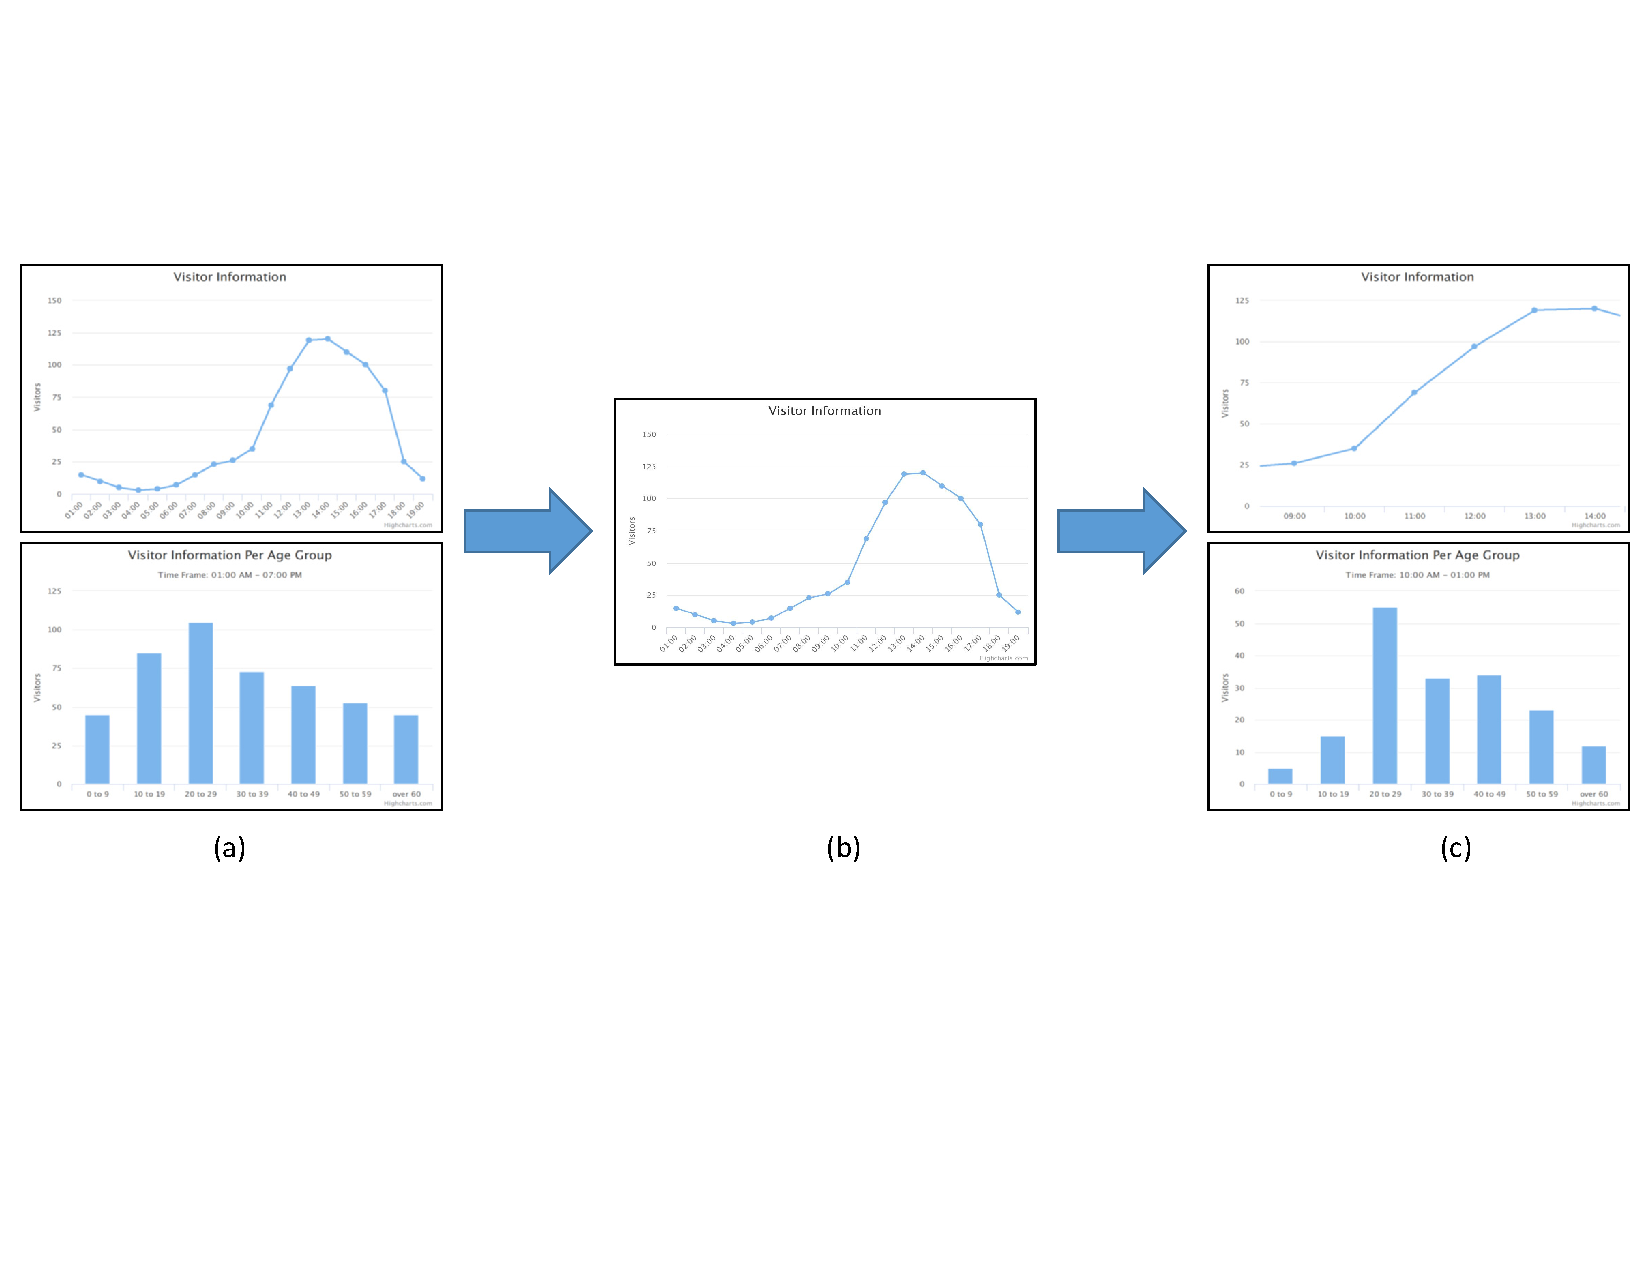
\includegraphics[width=\textwidth]{figures/highchart_final_a.pdf}
	\caption{Demonstration of interactive charts. The analyst's selection automatically updates the second plot (right).}
	\label{fig:vision}
\end{figure*}

\eat{
\begin{figure*}
	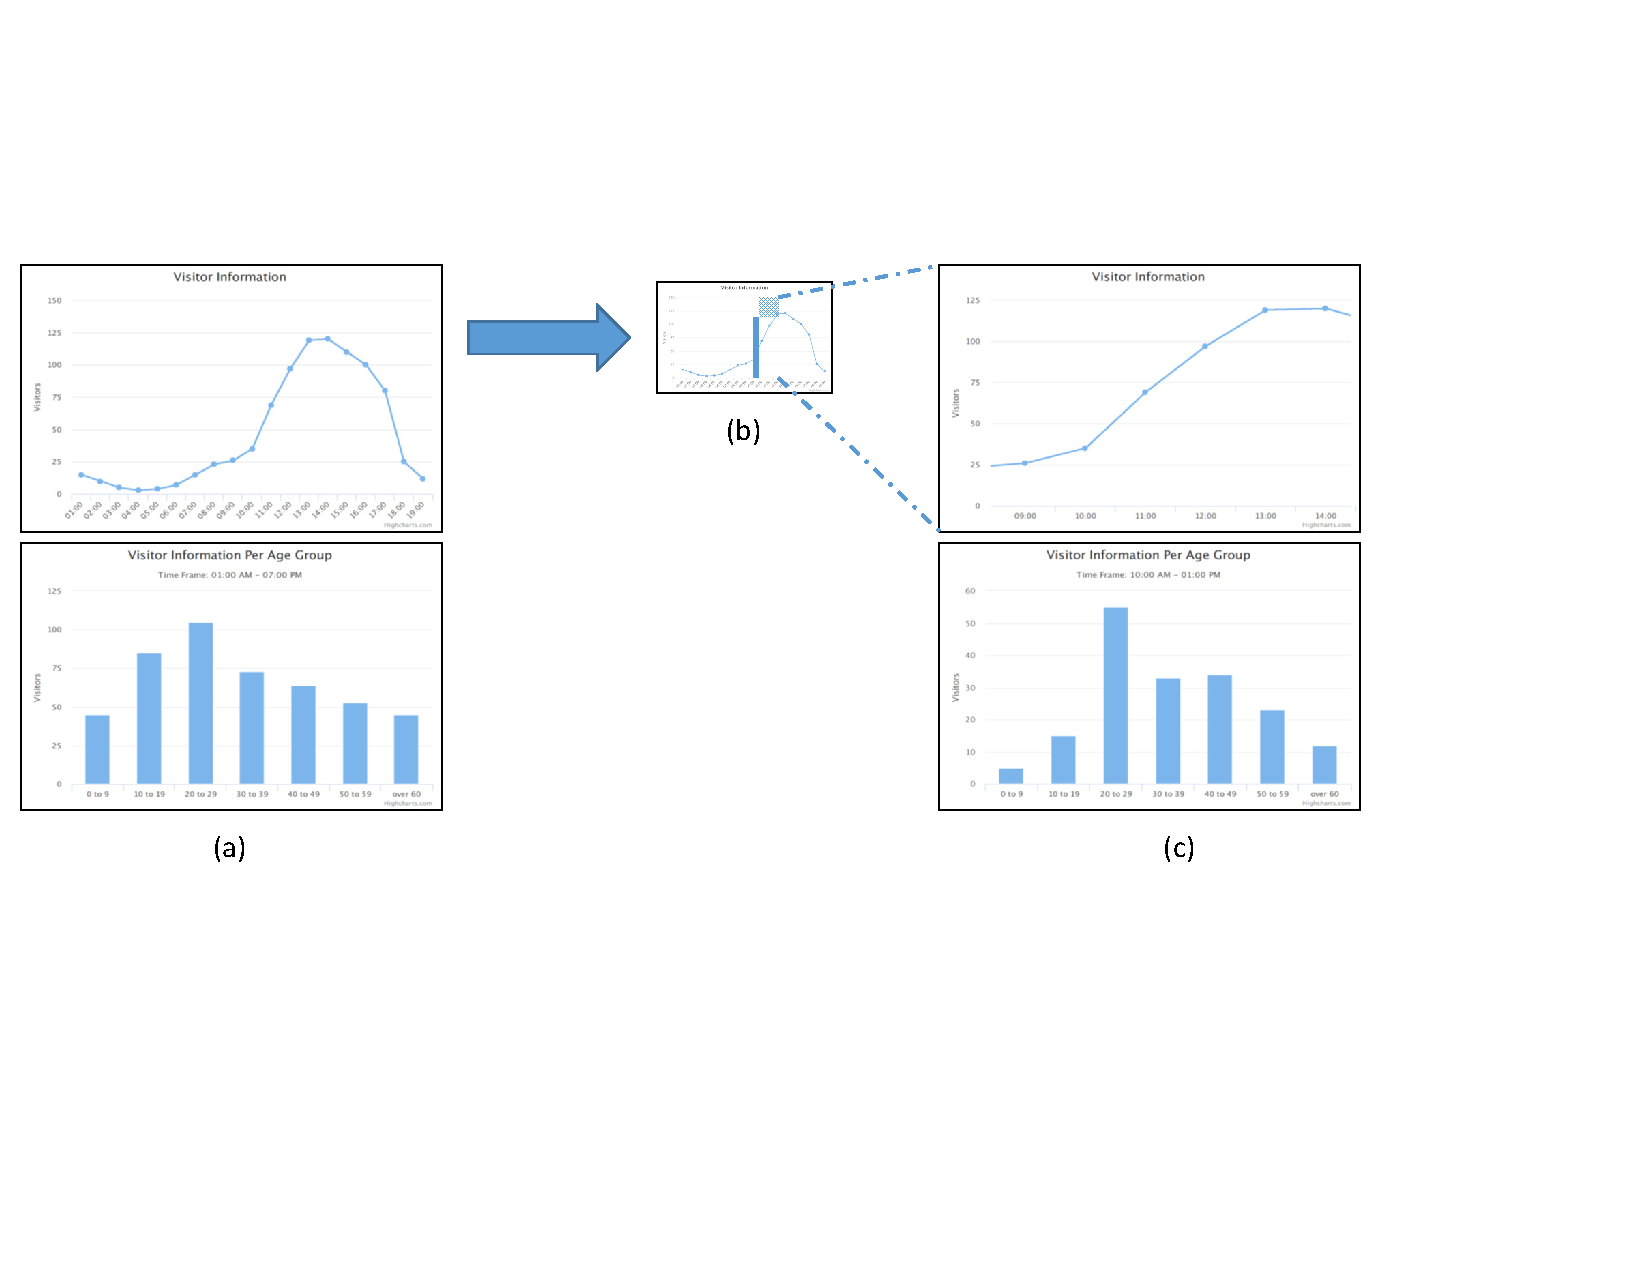
\includegraphics[width=\textwidth]{figures/highchart_final_b.pdf}
	\caption{Demonstration of interactive charts. The analyst's selection automatically updates the second plot (right).}
	\label{fig:vision}
\end{figure*}
}
\eat{
\remark{Ok I thought about it and I propose the following modifications in the paper structure (Nothing major - just moving text around to make it more readable): We begin with a good discussion about the vidette features that can help notebooks in section 2. We then show the entire walkthrough in one section (Section 3). By now, the reader knows what vidette can do so it will be easier to follow and understand the code we show.}
}
 \eat{
We address these issues, by extending interactive notebooks with the  {\projname} framework. {\projname} notebooks support a new template language capable of facilitating common data analysis tasks. The main contributions of this extension are:

\begin{itemize}
	\item \textit{Expressive template language:} Prior work, treats a page as a database view. Building on that, our template language goes beyond SQL query and view definition in both style and fundamental expressiveness. It is a mixture of query as well as web templating language that works on ordered (arrays) and semi-ordered (JSON) data. 
	\item \textit{Easy data retrieval:} Our framework supports communication with all major database types, such as Postgress, MongoDB, SQL etc, eliminating the need for individual DB drivers. Furthermore, using {\projname}, user access credentials for the database server(s) are stored in a configuration file, eliminating the embarassingly insecure practice of typing usernames and passwords in notebook cells vidible to everyone.
	\item \textit{Inline JSON operations:} The primary data structure used in {\projname} is JSON arrays. {\projname} combines the intuitive nature of JSON with the ability to write inline JSON operations, resulting in a clean, structured and readable code.
	\item \textit{Variable binding:} Analysts can easily ``bind'' variables using our template language. ``Binding'', results in automatic re-execution of notebook cells that contain those variables upon a change. {\projname} will trigger execution of the appropriate cells without any extra coding effort. As we show later, combined with inline JSON operations, binding becomes an incredibly versatile tool.

%	\item \textit{Declarative semantics:} {\projname} implements formal declarative \textit{Model-View-View-Model} (MVVM) semantics. \remark{Fill in why this is a good thing. I have no idea.}
%	\item \textit{Expressive template language:} Prior database work, treats a page as a database view. Building on that, our template language goes beyond SQL query and view definition in both style and fundamental expressiveness. It is a mixture of query as well as web templating language that works on ordered (arrays) and semi-ordered (JSON) data. 
%	\item We allow in-line declarative code directly in JSON...
\end{itemize}
}


%In this paper, we demonstrate the use of {\projname} via a walkthrough example. Specifically, we want to use website access data to plot an access count over time histogram. We also want to plot the recorded user demographics (with focus on age groups). We then want to have the ability to interact with the histogram plot and select a time region. This action should automatically update the second plot with the user demographics in the selected time window. 
%
%Without loss of generality, we assume a Jupyter server, where the analysts develop their notebooks and a different database server where data is stored. To retrieve the entirety of the required data, we have to query two different databases and join the returned JSON files. Figure ?? shows how our databases are organized. Our fictional analyst will perform the following high-level tasks:
%
%\begin{itemize}
%	\item Data retrieval from remote databases. 
%	\item Data curation: Join data and prepare for visualization.
%	\item Data visualization.
%\end{itemize}
%
%The remainder of this paper is organized as follows: Sections \ref{section:dataretrieval} -- \ref{section:visualization} present a direct comparison of using {\projname} and an imperative language such as Python in order to complete the tasks of our example. Throughout these sections, we demonstrate some of the main contributions of {\projname}. Section \ref{section:discussion} provides further discussion regarding our proposed extension and presents other useful aspects of it not used in our walkthrough. Finally, Section \ref{section:conclusion} concludes the paper.



\section{Running Example}


\begin{figure}[t]
  \centering
  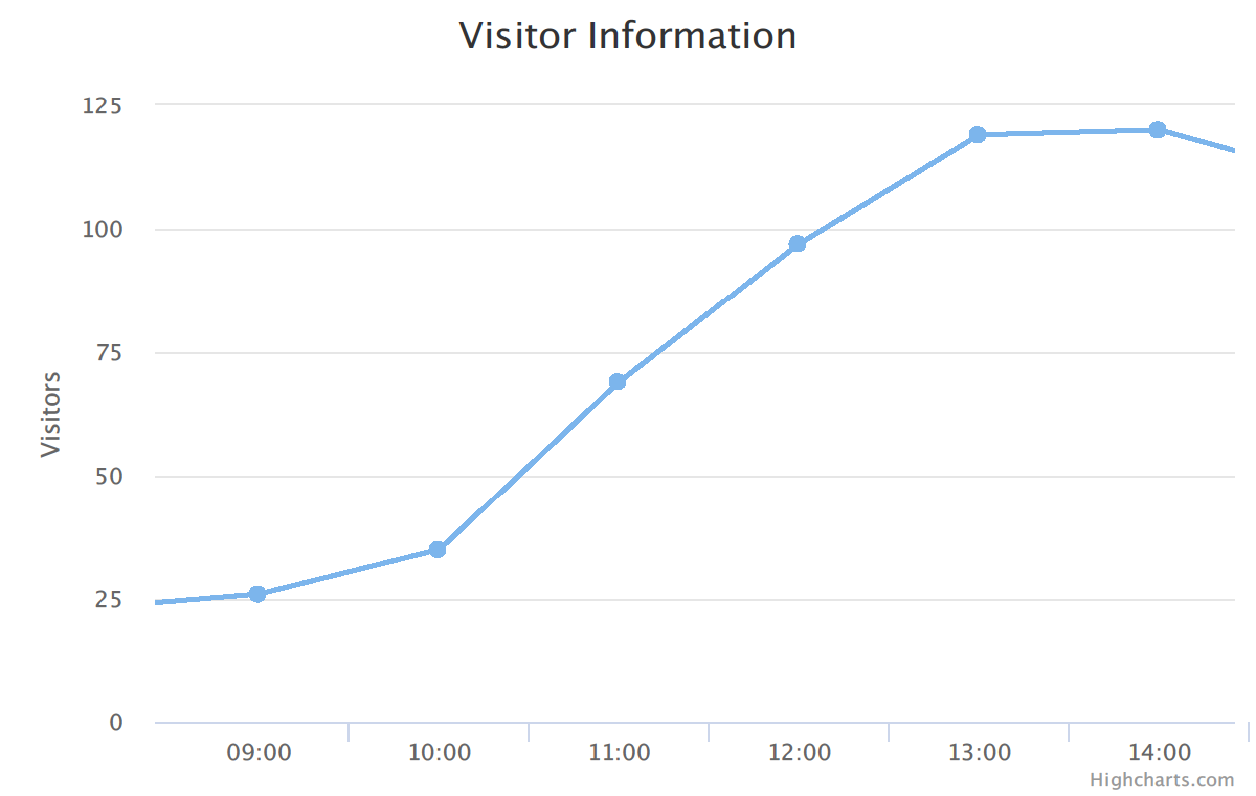
\includegraphics[width=0.8\columnwidth]{figures/first-line.png}
  \caption{Line chart showing visitors per hour}
\label{figure:first-running-example:first-line-chart}
  %\vspace*{\floatsep}% http://tex.stackexchange.com/q/26521/5764
   \vspace*{0.1cm}
  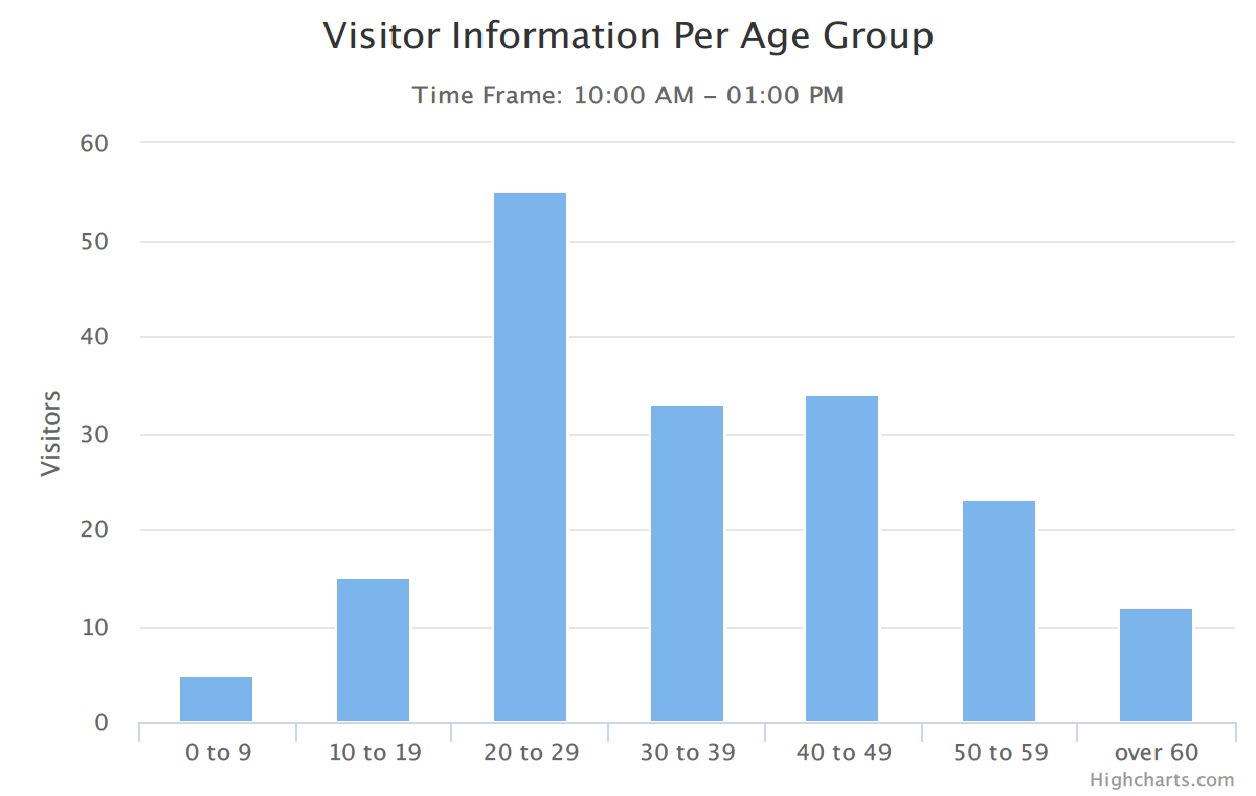
\includegraphics[width=0.8\columnwidth]{figures/first-bar.png}
  \caption{Bar chart showing age groups of visitors}
  \vspace{-10pt}
  \label{figure:first-running-example:first-bar-chart}
  
\end{figure}

\begin{table}
\begin{center}

\begin{tabular}{|c|c|c|c|c|}
\hline 
\multicolumn{5}{|c|}{Page Views} \\ 
\hline 
id & vid & url & time & date \\ 
\hline 
\end{tabular} 

\hfill

\begin{tabular}{|c|c|c|c|c|}
\hline 
\multicolumn{5}{|c|}{Visitors} \\ 
\hline 
vid & name & lastname & username & age \\ 
\hline 
\end{tabular} 

\end{center}
\caption{Schema description of the two tables in our database.}
\label{tab:schema}
\end{table}


In order to illustrate the issues with existing notebooks and describe the extensions in \projname\, we will use the following example of a potential analysis:

\begin{example}
Consider a data analyst, working for a news portal website. The analyst wishes to create a notebook that extracts and presents information about the demographics of the website's reader-base during particular hours. More specifically, the analyst wants to construct a chart showing the number of readers that visit the website during the day; then based on this information, she would like to extract the age groups of the visitors, during various hours of that day and present the results to the portal editor. Figure \ref{figure:first-running-example:first-line-chart} shows the graph that displays the number of visitors per hour in a line chart and Figure \ref{figure:first-running-example:first-bar-chart} displays the age groups of the visitors in a bar chart. By doing this, the analyst can convince the portal editor to publish more articles and advertisements that target particular age groups during hours in which they visit the portal the most, thus maximizing the portal's revenue and reader's satisfaction.
\end{example}

\eat{
\begin{figure}[ht]
  \centering
  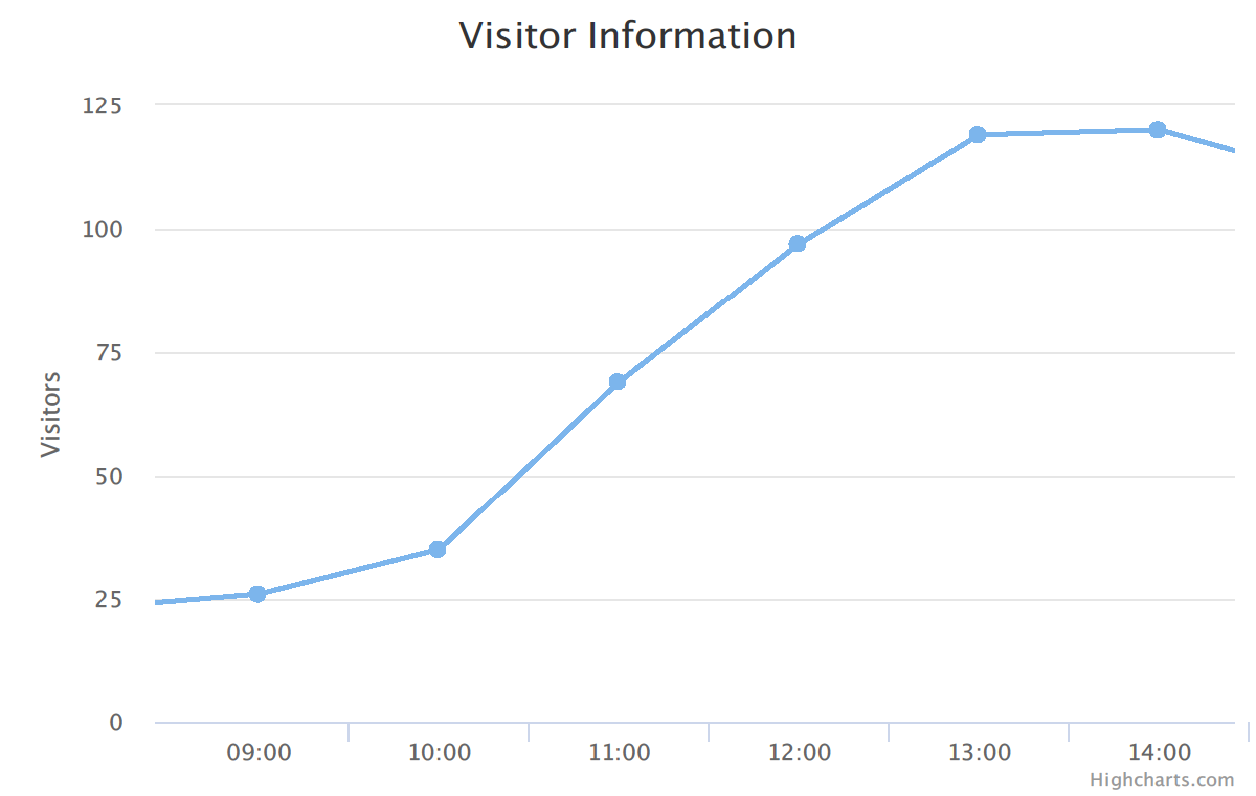
\includegraphics[width=0.8\columnwidth]{figures/first-line.png}
  \caption{Line chart showing visitors per hour}
\label{figure:first-running-example:first-line-chart}
  %\vspace*{\floatsep}% http://tex.stackexchange.com/q/26521/5764
   \vspace*{0.1cm}
  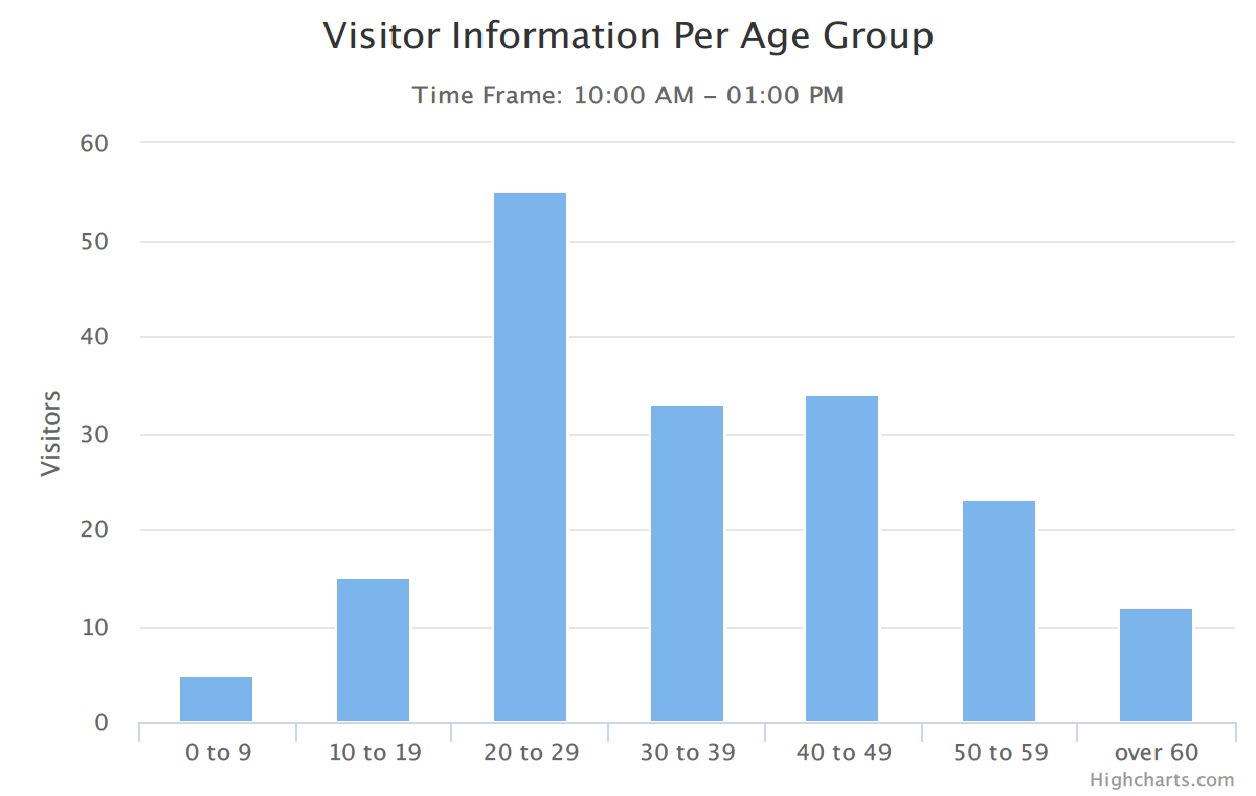
\includegraphics[width=0.8\columnwidth]{figures/first-bar.png}
  \caption{Bar chart showing age groups of visitors}
  \label{figure:first-running-example:first-bar-chart}
\end{figure}
}


For this analysis, we assume that the news portal maintains information about its reader-base in a Postgres database. Table \ref{tab:schema} shows a potential schema, that could be used for storing visitor information. The database contains two tables, namely ``Page Views" and ``Visitors"; table ``Visitors" contains information about each reader, such as the reader id, name, lastname, username and age. The table ``Page Views" maintains a tuple for each visit, and it consists of a visit id, the visitor id (foreign key referencing the visitor), the url of the visited page and the hour and date in which the user visited the website. The reader information could have been retrieved, with their permission, from various social media services (such as Facebook, Google etc). In order to construct this notebook, the data analyst must (a) retrieve  website access information from the database, by joining the two tables on the visitor id (b) generate a plot that shows the number of users that visit the website during the day, (c) issue a query that counts the number of visitors per age group, for each potential set of selected hours, and (d) create a bar chart that shows the number of visitors per age group. 





%\section{\projname\ Notebook Interface}
\label{section:programming-model}

In this section we present the interface of \projname\ notebooks as seen by a data analyst. The internal execution of the \projname\ engine, along with the automatically applied optimizations, is the topic of Section \ref{section:architecture}.  \\ 


\subsection{Data Retrieval}
\label{section:dataretrieval}

% Template and template instance figures
\begin{figure*}
\centering
%
%
\begin{minipage}[c]{6cm}
\begin{minipage}[c]{6cm}
\begin{code}
   sources : [ \{ 
     driver   : "postgres", 
     host     : "edu.db.domain", 
     expose   : [ \{
      schema : 'website_info', 
      tables: [visits, page_views] \} ]
     port     : 5432, 
     username : "dbadmin" 
     password : 'myP@ss'
   \}] 
\end{code}
\vspace*{-0.4cm}
\subcaption{DB Access Configuration file}
\vspace*{0.3cm}
\label{figure:source-config-file}
\end{minipage}
%
\begin{minipage}[c]{6cm}
\begin{code}
\textbf{<\% let} readings = 
   SELECT count(time) as visits, time
   FROM (SELECT * FROM page_views pv 
  	     join visitors v 
         on pv.v_id = v.vid) AS joined_table
   GROUP BY time 
   ORDER BY time ASC \textbf{\%>}
\end{code}
\vspace*{-0.4cm}
\subcaption{Data retrieval}
\label{figure:first-running-example:data-retrieval}
\vspace*{0.3cm}
\end{minipage}

\begin{minipage}[c]{6cm}
\begin{code}
readings = [
   \{visits: 15, time: '08:00'\}, 
   \{visits: 10, time: '09:00'\},
   \{visits: 25, time: '10:00'\},  ...]
\end{code}
\vspace*{-0.4cm}
\subcaption{Query Result}
\label{figure:running-example:query-result}
\vspace*{0.3cm}
\end{minipage}
%
\vspace*{0.6cm}
\end{minipage}
\hspace{2cm}
\begin{minipage}[c]{6cm}
\begin{minipage}[c]{7.5cm}
\begin{code}
  \directive{unit}{highcharts} \{
    title: 'Visitor information' ,
    xAxis : \{ 
      labels : ['08:00','09:00'...],
      min : '08:00'
      max : '22:00'
    \}
    series: [\{ data: [ \{y:15\}, \{y:10\}...] \}]
  \} \directive{end unit}{}
\end{code}
\vspace*{-0.4cm}
\subcaption{Unit with evaluated unit state}
\vspace*{0.3cm}
\label{figure:running-example:unit-body}
\end{minipage}
\begin{minipage}[c]{7.5cm}
\begin{code}
  \directive{unit}{highcharts} \{
    title: 'Visitor information',
    type: 'line'
    xAxis : \{ 
      labels : [
        \directive{for}{reading \textbf{in} readings} 
          \directive{print}{reading.time} 
        \directive{end for}{}],
      min : \directive{bind}{min_time},
      max : \directive{bind}{max_time}
    \}
    series: [\{
      data: [ \directive{for}{reading \textbf{in} readings}
          \{
            y  : \directive{print}{reading.count}
          \}
        \directive{end for}{} ]
    \}]
  \} \directive{end unit}{}
\end{code}
\vspace*{-0.3cm}
\subcaption{Template \texttt{temp\_view}}
\vspace*{0cm}
\label{figure:first-running-example:main-template}
\end{minipage}
\end{minipage}
\vspace*{-0.3cm}
\caption{Template, template instance, and UAS configuration file for the running example}
\vspace*{-0.3cm}
\end{figure*}


Data retrieval is one aspect where {\projname} shines. It enables the analyst to write inlined, source specific database queries without the use of any third-party libraries. In order to do this, data analysts have to generate a configuration file, containing information required for establishing a successful connection with the respective database systems. Figure \ref{figure:source-config-file} shows an example of the configuration file that is used for connecting to a postgres database that contains the data that will by used in our analysis. The configuration file must contain the type of the database system, the host name, port and the credentials that will be used for obtaining a connection. Additionally, it contains the database tables that will be accessible by queries. Only the tables that are explicitly defined in the configuration file will be accessible in the notebook. After this configuration file is imported, (which is done directly from the notebook's UI), it will be hidden from the UI and encrypted so that this information is no longer visible to the notebook reader.  Furthermore, as an added benefit, the schema of the accessible tables will be displayed on the UI, this allows the notebook user to get a glimpse of that information when generating the queries. 



Once this step is completed, the analyst is free to issue queries in order to access database systems. Specifically, she can use the notebook's UI in order to add a data-retrieval-cell and directly inline the query accessing any of they databases described in a configuration file. Figure \ref{figure:running-example:data-retrieval} contains a sample query that is used in our analysis. The query joins the two tables: $visitors$ and $page\_views$ on the id of the visitor, then groups the result on the $time$ attribute and runs a $count$ aggregate to count the visitors per unit of time. Lastly, it sorts the resulting dataset by time in ascending order. Figure \ref{figure:running-example:query-result} shows the result of the query. Notice that the result has been converted into a JSON array by \projname. In the next section we will show how to use this dataset to generate our first visualization, without the use of any imperative logic.

\subsection{Source Wrappers}
\label{subsection:source-wrappers}


\projname\ contains a set of source wrappers that enables data retrieval from various different sources both relational and non-relational. These source wrappers come pre-installed with \projname\ so that the notebook user will not have to take on any system administrator duties. The user simply provides the configuration file and writes the query in the language supported by each database system. The source wrapper uses that information to connect to the respective database system, retrieve the requested data, convert it into JSON format and make it available to the user. For database systems that do not contain tables with schema, the notebook user has to provide the respective record container under the "expose" attribute of the configuration file (i.e if the user accesses a MongoDB database, she will have to declare a collections of documents instead of database tables). Additionally, in cases when the accessed database system does not have a schema the notebook will simply display a small portion of the dataset, thus assisting the notebook user to compose queries.

\costas{Maybe put the last two sentences  in a side-note?}


\subsection{\projname\ Visual Units}
\label{section:visual Units}

\noindent To shield analysts from the laborious task of constructing visualizations, \projname\ abstracts out each visual component as a \projname\ \emph{visual unit} (or simply \emph{unit}). In the eyes of the analyst a visual unit is simply a black box that takes as input a JSON value that describes the visualization, namely, unit instance. The visual unit internally uses the unit instance to invoke the appropriate renderer calls that will generate the expected visualization. As such a particular instantiation of the unit  can be described as $\gl{<\% unit } U \gl{ \%> } v \gl{ <\% end unit \%>}$, where $U$ the type of the visual unit and $v$ the JSON value corresponding to the input of the unit. 


For instance, Figure \ref{figure:running-example:unit-body} shows a unit instance of type \texttt{highcharts}. The unit instance describes all the information that will be displayed in the visualization (such as the title of the chart, the labels on the x axis and so on). Each visual unit, comes with a unit instance schema that describes the format of the unit instance.


%Based on this idea, \projname\ abstracts out the entire visual page in the form of a logical specification, referred to as a \emph{template instance}. The template instance contains a description of the visual units that should be displayed in the page together with their inputs. For instance, Figure \ref{???} shows the template instance of our running example. It consists of two unit instances, one of type HighCharts and one of type \ref{???}. Each unit instance is denoted as $\gl{<\% unit } U \gl{ \%> } v \gl{ <\% end unit \%>}$, where $U$ the type of the visual unit and $v$ the JSON value corresponding to the input of the unit. A special type of unit is an HTML unit for displaying HTML content. An HTML unit instance is of the form $\gl{<\% html \%> } e_1 \ldots e_n \gl{ <\% end html \%>}$, where $e_1, \ldots, e_n$ are HTML elements.

\subsection{Template}
\label{section:template}


\eat{
\begin{figure}[t]
\centering
\scriptsize
\begin{tabular}{B}
\hline
 1  & \gn{template}             & \gp   & \gl{<\% template} \gn{template\_name} (\gn{param\_list}) \gl{\%>}                    \\
    &                           &       & ~~ \gn{let}*                                    \\
    &                           &       & ~~ \gn{unit}
\\
    &                           &       & \gl{<\% end template \%>}                                         \\
 2  & \gn{param\_list}			& \gp   & ( \gn{var\_name} (, \gn{var\_name})* )? 
\\ \hline
 3  & \gn{unit}         & \gp   & \gl{<\% unit} \gn{unit\_class} \gl{\%>}               \\
    &                           &       & ~~ \gn{value}                                         \\
    &                           &       & \gl{<\% end unit \%>}                                 \\
 4  & \gn{value}                & \gp   & \gn{jsonpp\_value} %\text{(see Figure~\ref{figure:bnf-value})} 
\\
 5  &                           & \gd   & \gn{unit}                                     
\\
 6  &                           & \gd   & \gn{print}                                                        \\
 7  &                           & \gd   & \gl{[} \gn{for} \gl{]}                                                                                \\
 8  &                           & \gd   & \gl{<} \gn{for} \gl{>}                                                                                \\
 9  &                           & \gd   & \gn{if}                                                                                 \\
  
 10  &                           & \gd   & \gn{bind}                                                         \\
11  &                           & \gd   & \gl{\{} \gn{event}*                                               \\
    &                           &       & ~~ (\gl{\textquotedbl}\gn{string}\gl{\textquotedbl} 
                                             \gl{:} \gn{value}                                              \\
    &                           &       & ~~ (\gl{,} \gl{\textquotedbl}\gn{string}\gl{\textquotedbl} 
                                             \gl{:} \gn{value})* )? \gl{\}}                                           \\ \hline
12  & \gn{let}                 & \gp   & \gl{<\% let} \gn{var\_name} \gl{=} \gn{expr} \gl{\%>}            
\\
13  & \gn{print}                & \gp   & \gl{<\% print} \gn{expr} \gl{\%>}                                 \\
14  & \gn{for}                  & \gp   & \gl{<\% for} \gn{var\_name} \gl{in} \gn{expr} \gl{\%>}           
\\
    &                           &       & ~~ \gn{let}*                                    \\
    &                           &       & ~~ \gn{value}
\\
    &                           &       & \gl{<\% end for \%>}                                              \\
    
14  & \gn{if}                  & \gp   & \gl{<\% if}  \gn{expr} \gl{\%>}           
\\
    &                           &       & ~~ \gn{value}
\\
 &                           &       & ~~ (\gl{<\% elif}  \gn{expr} \gl{\%>} 
 
\\
 &                           &       & ~~ \gn{value})*    
 \\
 &                           &       & ~~ (\gl{<\% else}  \gl{\%>} 
 
\\
 &                           &       & ~~ \gn{value})?    
\\
    &                           &       & \gl{<\% end if \%>}                                              \\
15  & \gn{bind}                 & \gp   & \gl{<\% bind} \gn{var\_name} = \gn{expr} \gl{\%>}                             \\
16  & \gn{event}                & \gp   & \gl{<\% event} \gn{event\_name} \gn{action\_name} \gl{\%>}        \\
17  & \gn{expr}                 & \gp   & \gn{js\_expression}                                               \\
18  &                           & \gd   & \gn{source\_expression}                                                   \\
19  &                           & \gd   & \gn{json\_path}                                                   \\
\hline
\end{tabular}
\caption{BNF Grammar for Templates}
\label{figure:bnf-template}
\end{figure}
}


\emph{Templates} are declarative specifications that can be used to generate \projname\ variables or unit instances. The template language supports a set of \emph{template directives}, all of which operate on the JSON datamodel. These directives are used to describe computation, define variables and set up data collection. Due to lack of space we do not include a figure containing a formal BNF grammar for the template language, instead we simply describe each of them in detail and provide a concrete example that illustrates their use. 




\noindent {\bf Defining variables.} A template may define variables that are added to the notebook's environment so that they can be used in subsequent computation. The $\gl{<\% let } x \gl{ = } E \gl{ \%>}$ directive defines variable $x$ and assigns to it the result of the expression $E$. $E$ can denote three types of expressions: path navigation on JSON data, invocation of a python function that performs computation by using as input and output JSON values or a source-specific language (such as a SQL query). For instance, the template shown in Figure \ref{figure:first-running-example:data-retrieval} employs a \gl{let} directive to create a variable \texttt{readings} containing the visitor information that will be displayed in the chart (retrieved from a relational DBMS through an SQL query).

\noindent {\bf Reporting data.} Value assignments and iterations over collections are specified by using the \gl{print} and \gl{for} directives. The $\gl{<\% print } E \gl{ \%>}$ directive evaluates the expression $E$ and returns the result, while the $\gl{<\% for } x \gl{ in } E \gl{ \%> } B \gl{ <\% end for \%>}$ directive specifies that variable $x$ iterates over the result of $E$ and, in each iteration, it instanciates the body $B$ of the \gl{for} loop. In Figure \ref{figure:first-running-example:main-template}, in lines 7-9 and 14-18 a \gl{for} directive is used to iterate over the readings retrieved from the database and for each reading, it generates a new JSON value, with the use of the \gl{print} directive. Particularly, in line 8 the template generates a string (the time label), which is added to the labels array (which contains the labels that will appear on the x axis of the chart). In lines 15-17 it generates a JSON object of the form \{y: ...\} and adds it to the data array. The data array in highcharts contains the points that will appear in the chart.

\noindent {\bf Collecting data.} In addition to specifying how to compute a template instance, the template's \gl{bind} directive allows the analyst to specify user input collection. Specifically, the $\gl{<\% bind x} \gl{ \%>}$ directive describes a two-way bind that will be created between the part of the unit instance appearing on its left side and to variable $x$. For instance, in Figure \ref{figure:first-running-example:main-template} in lines 10-11 we create a two-way binding between the min and max boundaries of the chart and the min and max values of the time labels that have been retrieved (namely min\_time and max\_time). While the user interacts with chart he can select a particular region in the chart which in turn updates the values $min\_time$ and $max\_time$. This event invokes an internal propagation algorithm (which will be described in the next section) which triggers the revaluation of the \projname\ statements that use the values $min\_time$ and $max\_time$ in other parts of the notebook.






%\section{Introduction}
\label{section:introduction}

\noindent \textbf{Contributions} We describe the following contributions of \projname:
\begin{compact_item}

%

\item \textit{Declarative Semantics:} We present a formal declarative MVVM semantics for \projname. To the best of our knowledge, this is the first formal presentation of MVVM declarative semantics by an MVVM framework. \yannis{What extra do we offer in light of CIDR11 to the semantics?} 
\costas{Fundamentally, they are both diff driven application frameworks... Some differences are that the CIDR11 and SIGMOD10 version: 1.the template language was written in XML which was more verbose and therefore needed more effort to be written (more characters per line and more total lines of code for the same template instance). 2.Additionally, since template functions were not supported, the app developer often had to inline complex SQL++ queries in the template to ``massage" the data appropriately. 3. Delta functions were not supported. Overall templates appeared more convoluted compared to the current version and therefore they were harder to follow. For more differences check respective file in Notes folder (at the root of the repo)} \yannis{A large difference between CIDR11 and current work is the aim to easily interface with JavaScript. This is behind the functions in the template language, the interfacing of JavaScript components, the JavaScript actions and (the missing) easy programming model for accessing JavaScript data (the latter can stay for journal or OOPSLA)} Hence, the declarative semantics of \projname\ can also serve as an introduction to the semantics of MVVM at large, and to the semantics of \angular\ and other MVVM frameworks, after one accounts for their limitations.
%
\item \textit{Expressive Template Language:} While we draw from prior database research work, which treats the page as a database view, the template language goes beyond SQL query and view definitions in both style and fundamental expressiveness \yannis{Good point for a journal publication but on VLDB suffers from CIDR comparisons. The reason behind the higher expressiveness is new.}: It is a mixture of query language and web templating language that works on ordered data (arrays) and semi-structured data (JSON) \costas{JSON encompasses the concept of arrays/ ordered data}and is expressive enough to cover many common transformations without requiring the use of additional imperative JavaScript code. Notably, it is more expressive than the language of \angular, due to reasons pertaining to differences in their incremental rendering algorithms. \yannis{Cannot be quickly backed up by the example. Two nested loops may be hard but a for/if combo is doable.} \costas{How would it be backed up by example? We would have to introduce Angular and \projname\ templates in the intro, wouldn't we?} Furthermore, besides visualization, the templates can also input data and catch events/activate actions \costas{actions have not been defined}, as a complete web application development framework should do.

%
\item \textit{Incremental Rendering:} The incremental rendering problem has similarities to Incremental View Maintenance (IVM) but also poses distinct new challenges due to (1) template language features that have not received attention by the database community, and (2) unlike IVM whose goal is to update a target materialized view, the incremental rendering algorithm is a \textit{diff propagation} algorithm that results into a sequence of calls to the rendering methods of (the usually 3rd party) components. \yannis{A diff and its resulting rendering method call should have been demonstrated in the context of the example.} Pertaining to Item~(1) \projname\ solves the following diff propagation problems:
\begin{compact_enum}
\item \textit{Handling Arrays:} Arrays are prime citizens of the data model. Therefore we reconsidered what is the appropriate language for describing diffs, so that diffs on arrays are included. \costas{What do we mean when we say ``language" for describing diffs}\yannis{Current example has no motivation for insertion in the middle of array, which is where problems happen.}Second we developed algorithms for propagating such diffs.   
%


\item \textit{Black-box functions in Template:}\yannis{no example of a function either. It need not be the first example but I think there is just no example.} In the rare cases where the out-of-the-box expresiveness of the template language is not enough, the developer can include Javascript function invocations in her template. \projname\ offers a pay-as-you-go approach to the efficient diff propagation through JavaScript functions that may be part of the template: The developer may provide nothing (but the function itself), in which case the diff propagation algorithm will still work but may be slow\costas{Let's avoid the word slow, let's just say it wouldn't work ``incrementally", which is the more efficient.}, as it will be re-evaluating the function. Alternately, the developer may provide one or more diff management functions, which are suggested to her by \projname\ and lead to more efficient diff propagation. \costas{We should also mention that we provide some of these functions out-of-the-box (e.g sortby, groupby etc...)}\yannis{IMPORTANT: we need to discuss how this differs from angular's pay-as-you-go} \costas{Angular does not provide something similar to \projname's delta functions, so there's nothing to pay as you go}
%\costas{The IVM algorithm will be fast, the function re-evaluation may be slow (We should make it clear to the reader that the bottleneck isn't the template IVM algorithm but the user defined function...). That's why we enable the function developer to provide auxiliary delta functions that update the logical page more efficiently. }
%

\item \textit{Loops in Templates} \projname\ provides diff propagation over loop structures.  \costas{Why is that a big deal? This bullet doesn't illustrate why that's challenging or interesting...}\yannis{would be far more convincing with fors and ifs}

% 
\end{compact_enum}
%
The \projname\ incremental rendering also solves the following problems pertaining to its need to translate diffs into rendering method calls. \yannis{as said above, problems should have memorable names and do not repeat the whole description continously} \costas{refer to dictionary spreadsheet} \url{https://docs.google.com/spreadsheets/d/1pn6EPZUnz\_3Tc3e7FnveRxQXcs2uRqD0znERjI0-g0o/edit#gid=0}
\begin{compact_enum}

\item \textit{Easy wrapping of 3rd party components} A novel triggering algorithm enables the easy and pay-as-you-go wrapping of Javascript visualization rendering methods. In particular, the developer in charge of wrapping a visualization component is only tasked with specifying the single diff that a rendering method handles. \costas{This sentence doesn't make sense: ``(The developer specifies the) single diff that a rendering method handles". The developer does not specify diffs, he specifies renderer wrappers and diff signatures (refer to dictionary). The number of renderer wrappers he needs to specify is anything between two (construct-destruct) and the total number of renderers supported by the visualization library} \yannis{Needs example. Recall, earlier we introduced a diff and a corresponding renderer. Here we should change the assumption on renderer or the diff so that we can show simulation.}Therefore the size of the specification \costas{what specification?}is proportional to the number of rendering methods she wishes to wrap, as opposed to the number of the possible kinds of diffs, which is typically far larger. \costas{the latter number is: supported-diff opcodes X potential targets in unit instance} \yannis{tell the number that shows how many diffs exist in our example. You don't have to substantiate yet why so many. The substantiation will come much later once we have shown the unit's "schema" and have explained how many kinds of diff exist.
The most impressive introductions say "without my technique it would be N and with my technique it is M that is an order of magnitude below"} \costas{I don't follow. Why do we need to specify the number of possible diffs. When reading this section it feels like we're comparing our system with a system similar to ours that does not support simulation. Angular does not work with diffs, so this is somewhat pointless.} When a diff is produced that does not correspond directly to a rendering method, \projname\ discovers how to indirectly support it by \textit{simulating} the missing rendering method with existing wrapped rendering methods. \costas{we should add something like: ``This automation significantly simplifies the process of unit wrapping. Since competing frameworks do not provide a similar feature, unit developers are often required to manually perform it manually. This negatively impacts both the amount of time that needs to be spent in unit wrapping and the amount of lines of code that need to be written"}Lines-of-code experiments show the advantage of \projname\ in 3rd party wrapping productivity.

\eat{
\costas{The reasons why Angular directives need more lines are:
Actually the problem, arises when two renderers exist, one at a deeper level then the other. In such cases, Angular directive developers have to install a deep watcher at the higher level and manually compare the parts that correspond to more ``specific" renderers, to identify what changed. This happens to avoid the invocation of multiple renderers, which would be a direct result of}
}
%
\item \textit{Managing Direct Updates and Provenance Heterogeneity} \projname\ treats update diffs as first-class citizens, as opposed to simulating updates by insert-delete combinations. \costas{Not sure why we mention this, Angular directives don't need to simulate updates diffs with insert-delete diffs. Is this something that other IVM algorithms do not support?} This feature leads to higher performance and also superior UI behavior, when the visualization components provide update renderer methods. It also creates a need for keeping track of the provenance of each part of the visualization, so that it can be identified and updated. Notice that provenance has to be converted into terms that the 3rd party component understands, creating a need for special conversion data structures and algorithms. \yannis{Needs support of the example, both on the update and on the provenance. (The current example is an insertion and does not have any provenance problem.)}
\end{compact_enum}
%
\item \textit{Superior performance over other MVVM frameworks:} A net effect of the algorithms is that the client-side incremental rendering algorithm achieves better Big-O algorithmic complexity than the incremental rendering algorithm of \angular\ and also ouperforms it in the presented experiments.
%
\end{compact_item}

{\bf Paper Outline.} \yannisk{Revise after the sections have been finalized} The paper is structured as follows: In Section \ref{section:programming-model} we explain the structure of a \projname\ application as seen by an application developer. Section \ref{section:architecture} describes \projname's internal architecture, while Sections \ref{section:template-ivm}-\ref{section:visual-ivm} describe the incremental view maintenance algorithms that power the framework. Section \ref{section:experiments} compares the performance and productivity gains of the proposed system against the state of the art. Finally, Sections \ref{section:related-work} and \ref{section:conclusion} discuss related work and conclude the paper, respectively.
%\section{{\projname} Architecture}
\label{section:arch}

SOME INTRO TEXT (1-2 paragraphs)

\subsection{Source Wrappers}

\subsection{Visual Units}

\subsection{Template(?)}

\subsection{Interactive Interface}

\remark{Costa, the algorithms you have for this section are completely unreadable. I don't think it helps anyone who reads it and it will take forever if we actually want to explain it in text. I assume (hope) these are algorithms that run in the background (under the hood vidette functions) and not something the analyst needs to write. If that's the case, let's describe the operation of those functions logically in text. If the analyst actually needs to write that code, I don't think we have a submit-able paper here.}

%\section{Walkthrough Example}

DESCRIBE THE PROBLEM AGAIN WITH MORE DETAIL

\subsection{Data Retrieval}
Just move what we already have in the Data retrieval section here.

\subsection{Simple Visualization}
Here we show simple non-interactive visualization using vidette. We get a chance to say how intuitive everything is and how awesome it is that we can inline functions in these units.

\subsection{Interactive Visualization}
Here we show the modifications needed to go from simple to interactive visualizations. This way we point out that going from naive to advanced visualizations take minor modifications in the units and everything is taken care of under the hood.

%\section{Data Retrieval}
\label{section:dataretrieval}

% Template and template instance figures
\begin{figure*}
\centering
%
%
\begin{minipage}[c]{6cm}
\begin{minipage}[c]{6cm}
\begin{code}
   sources : [ \{ 
     driver   : "postgres", 
     host     : "edu.db.domain", 
     expose   : [ \{
      schema : 'website_info', 
      tables: [visits, page_views] \} ]
     port     : 5432, 
     username : "dbadmin" 
     password : 'myP@ss'
   \}] 
\end{code}
\subcaption{DB Access Configuration file}
\label{figure:source-config-file}
\end{minipage}
%
\begin{minipage}[c]{6cm}
\begin{code}
\textbf{<\% let} readings = 
   SELECT count(time) as visits, time
   FROM (SELECT * FROM page_views pv 
  	     join visitors v 
         on pv.v_id = v.vid) AS joined_table
   GROUP BY time 
   ORDER BY time ASC\textbf{\%>}
\end{code}
\vspace*{-0.3cm}
\subcaption{Template instance}
\label{figure:running-example:main-template-instance}
\vspace*{0.3cm}
\end{minipage}

\begin{minipage}[c]{6cm}
\begin{code}
readings = [
   \{visits: 15, time: '08:00'\}, 
   \{visits: 10, time: '09:00'\},
   \{visits: 25, time: '10:00'\},  ...]
\end{code}
\vspace*{-0.3cm}
\subcaption{Template instance}
\label{figure:running-example:main-template-instance}
\vspace*{0.3cm}
\end{minipage}
%
\end{minipage}
\hspace{1cm}
\begin{minipage}[c]{8.5cm}
\begin{code}
\directive{template}{temp\_view()}
  \directive{import}{functions}
  \directive{import}{actions}

  \textbf{<\% let} readings = select t.temp
                    from db.temperature as t
                    order by timestamp \textbf{\%>}
  
  \directive{unit}{highcharts}
  \{\eat{
    chart: \{
      renderTo: 'container',
      zoomType: 'x'
    \},}
    title: \{ text: 'Temperature monitor' \}, \eat{
    plotOptions: \{
      series: \{
        turboThreshold: 5000000
      \}
    \},
    subtitle: \{
      text: 'Using the experimental Highcharts Boost module'
    \},
    tooltip: \{
      valueDecimals: 1
    \},}    
    series: [\{
      data: [
        \directive{for}{reading \textbf{in} readings}
          \{
            y    : \directive{print}{reading.temp},
            color: \directive{print}{toHex(reading.temp, threshold)}
          \}
        \directive{end for}{}
      ],
      lineWidth: 1
    \}],
    \gl{<\% event} onSelection redrawSelected() \gl{\%>}
  \}
  \directive{end unit}{}
  
  \directive{unit}{slider}
  \{
    min  : 0,
    max  : 10000,
    value: \directive{bind}{threshold = 65}
  \}
  \directive{end unit}{}
\directive{end template}{}
\end{code}
\vspace*{-0.3cm}
\subcaption{Template \texttt{temp\_view}}
\vspace*{0.3cm}
\label{figure:running-example:main-template}
\end{minipage}
\caption{Template, template instance, and UAS configuration file for the running example}
\end{figure*}


\remark{It might be a good idea to merge these 3 sections into 1 called ``Walkthrough example'' or something like that. Depends on how large these sections become.}



Data retrieval is one aspect where {\projname} shines. The analyst is given the ability to write clean and readable database queries (?? - Is there a better name - ??) \costas{yep that's how we call them...} in order to retrieve data from the remote server. In a Python implementation, analysts need to perform a series of tasks before being able to retrieve data. Some of these tasks potentially fall way beyond the skill set of the average data analyst. 

\costas{We should also say that we simplify file imports. For cases, when the data analysts wants to use csv or json files from their local computer, they can use an import button, which is part of our UI, to upload them to the notebook server. After that step is completed we trigger a function that automatically converts this file to JSON and we assign it to a \projname\ variable, so that it can be used in the notebook. Currently, this task requires ssh-ing or scp-ing the files to the notebook server, and potentially moving files to the directive/file-system that is seen by the notebook, which also requires system administrator-linux knowledge}



First, our analyst needs to install and configure database drivers. This step will either introduce a dependency between the analyst and some system administrator, or the analyst will need to have the required access rights in order to perform the installation. The later can be a security concern or can lead to corrupted systems if not performed correctly. The complexity of this step increases as the types of databases our analyst wants to access increases. If for example we have data stored in a MongoDB and a SQL database, two drivers will need to be installed.

Once the system is configured, the analyst then needs to read lengthy documentation documents in order to properly issue queries to the databases via imperative code.

Finally, when implemented in a Jupyter notebook, the analyst's credentials for the database server might lie on plain sight to anyone who has access to the notebook, disrupting the valuable ease of results communication through notebooks.

{\projname} addresses each one of the aforementioned imperative code issues efficiently: The analyst generates a configuration file, containing information required for obtaining a successful connection with the respective database systems. Figure \ref{figure:source-config-file} shows an example of a configuration file for accessing a postgres database. It contains the type of the database system, the host name, port and the credentials that will be used obtaining a connection. Additionally, it contains the database tables that will be accessible by queries, only the tables that are explicitly defined in the configuration file will be accessible by \projname. After this configuration file is imported, by using the user interface of \projname\, it will be encrypted so that this information is no longer visible to the notebook reader. Furthermore, as an added benefit, the schema of the accessible tables will be displayed in the UI, in order to allow the notebook user to get a quick glimpse, when generating the queries. For database systems that do not contain schema, \projname\ will simply display a small portion of the dataset instead.

 \remark{Diko sas!}

As a result, credentials are no longer directly visible to the notebook reader. As an added benefit, these configuration files contain a description of the schema of each table, allowing the notebook user to get a quick glimpse of the database's structure as soon as connection is established.

\remark{Technical details by Costas Z. follow. All rise.}



%\section{Data Curation}
\label{section:datacuration}

DATA CURATION

%\section{Visualization}
\label{section:visualization}



% % Template and template instance figures
\begin{figure*}
\centering
%
\begin{minipage}[c]{8.5cm}
\begin{code}
\directive{template}{temp\_view()}
  \directive{import}{functions}
  \directive{import}{actions}

  \textbf{<\% let} readings = select t.temp
                    from db.temperature as t
                    order by timestamp \textbf{\%>}
  
  \directive{unit}{highcharts}
  \{\eat{
    chart: \{
      renderTo: 'container',
      zoomType: 'x'
    \},}
    title: \{ text: 'Temperature monitor' \}, \eat{
    plotOptions: \{
      series: \{
        turboThreshold: 5000000
      \}
    \},
    subtitle: \{
      text: 'Using the experimental Highcharts Boost module'
    \},
    tooltip: \{
      valueDecimals: 1
    \},}    
    series: [\{
      data: [
        \directive{for}{reading \textbf{in} readings}
          \{
            y    : \directive{print}{reading.temp},
            color: \directive{print}{toHex(reading.temp, threshold)}
          \}
        \directive{end for}{}
      ],
      lineWidth: 1
    \}],
    \gl{<\% event} onSelection redrawSelected() \gl{\%>}
  \}
  \directive{end unit}{}
  
  \directive{unit}{slider}
  \{
    min  : 0,
    max  : 10000,
    value: \directive{bind}{threshold = 65}
  \}
  \directive{end unit}{}
\directive{end template}{}
\end{code}
\vspace*{-0.3cm}
\subcaption{Template \texttt{temp\_view}}
\vspace*{0.3cm}
\label{figure:running-example:main-template}
\end{minipage}
%
\hspace{1cm}
%
\begin{minipage}[c]{6cm}
%
\begin{minipage}[c]{6cm}
\begin{code}
\directive{unit}{highcharts}
\{\eat{
  chart: \{
    renderTo: 'container',
    zoomType: 'x'
  \},}
  title: \{ text: 'Temperature monitor' \},\eat{
  plotOptions: \{
    series: \{
      turboThreshold: 5000000
    \}
  \},
  subtitle: \{
    text: 'Using the experimental Highcharts Boost module'
  \},
  tooltip: \{
    valueDecimals: 1
  \},}    
  series: [\{
    data: [
        \{ y: 55, color: '#359435' \},
        \{ y: 57, color: '#359823' \},
        \{ y: 56, color: '#359533' \},
        \{ y: 53, color: '#359220' \}
    ],
    lineWidth: 1
  \}]
\}
\directive{end unit}{}

\directive{unit}{slider}
\{
  min : 0,
  max : 10000,
  value: 65
\}
\directive{end unit}{}
\end{code}
\vspace*{-0.3cm}
\subcaption{Template instance}
\label{figure:running-example:main-template-instance}
\vspace*{0.3cm}
\end{minipage}
\begin{minipage}[c]{6cm}
\begin{code}
   sources : [ \{ 
     driver   : "postgres", 
     host     : "localhost", 
     port     : 5432, 
     aliases  : [\{db : "sensorDb"\}]
     username : "dbadmin" 
   \}] 
\end{code}
\subcaption{UAS configuration file}
\label{figure:uas-config-file}
\end{minipage}


%
\end{minipage}
\caption{Template, template instance, and UAS configuration file for the running example}
\end{figure*}

% Lines of different concepts in the template and template instances
\newcommand{\templateinstanceline}[1]{%
    \IfEqCase*{#1}{%
    {highcharts-unit-instance}{lines~1-14}%
    {slider-unit-instance}{lines~16-22}%
    }[\errmessage{Unable to ref #1 for template instance}]%
}%

\newcommand{\templateline}[1]{%
    \IfEqCase*{#1}{%
    {highcharts-unit}{lines~9-24}%
    {slider-unit}{lines~26-32}%    
    {print-y}{line~16}%
    {print-color}{line~17}%
    {for}{lines~14-19}%
    {let}{lines~6-8}%
    {bind}{line~30}%
    }[\errmessage{Unable to ref #1 for template}]%
}%

\yannis{About Figure \ref{figure:running-example:main-template}: Why the importing is on the template? The actions may not be template specific. Same for the functions.}

\costas{Yes, the template needs to be changed.}

\yannis{About Figure \ref{figure:running-example:main-template}: The total absence of html and/or any form of unit testing hurts the idea that we do pages. }

\costas{The two units should be wrapped by an HTML unit. I believe this was done like that to avoid an extensive description on fragmentation.}

\yannis{About Figure \ref{figure:running-example:main-template}: The query suspiciously lacks any window }

\costas{The application shows historic data, it doesn't show a particular window. The user however can use the chart to zoom into some time window, to explore the data.}

\yannis{About Figure \ref{figure:running-example:main-template}: Query almost covers the provenance heterogeneity problem behind time stamp.}

\yannis{About Figure \ref{figure:running-example:main-template-instance} slider unit: May be good to have a non-initial value and talk about it.}



\begin{figure*}
\centering
%
%
\begin{minipage}[c]{7.5cm}
%
\begin{minipage}[c]{7.5cm}
\begin{code}
\textbf{<\% let} age_groups = 
   SELECT agegroup, count(*) AS total 
   FROM (SELECT CASE
    WHEN age BETWEEN 0 AND 9 THEN '0 to 9'
    WHEN age BETWEEN 10 and 19 THEN '10 to 19'
     ...
    FROM (SELECT * FROM page_views pv join visitors v 
          on pv.v_id = v.vid where time BETWEEN 
          \textbf{<\%=min_time} and \textbf{<\%=max_time}) joined_data) jd
   GROUP BY agegroup  
   ORDER BY agegroup ASC \textbf{\%>}
\end{code}
\vspace*{-0.3cm}
\subcaption{Data retrieval}
\label{figure:running-example:age-group-data-retrieval}
\vspace*{0.3cm}
\end{minipage}

\begin{minipage}[c]{7.5cm}
\begin{code}
age_groups = [
   \{age_group: '0 to 9', total: 12\}, 
   \{age_group: '10 to 19', total: 67\},
   \{age_group: '20 to 29', total: 84\},  ...]
\end{code}
\vspace*{-0.3cm}
\subcaption{Query Result}
\label{figure:running-example:age-group-query-result}
\vspace*{0.3cm}
\end{minipage}
%
\end{minipage}
\hspace{1cm}
\begin{minipage}[c]{6cm}

\begin{minipage}[c]{8.5cm}
\begin{code}
  \directive{unit}{highcharts}
  \{
    title: 'Visitor information',
    xAxis : \{ 
      labels : [
        \directive{for}{v \textbf{in} age_groups} 
          \directive{print}{v.age_group} 
        \directive{end for}{}]
    \}
    series: [\{
      data: [ \directive{for}{v \textbf{in} age_groups}
          \{
            y  : \directive{print}{v.total}
          \}
        \directive{end for}{} ]
    \}]
  \}
  \directive{end unit}{}
\end{code}
\vspace*{-0.3cm}
\subcaption{Template \texttt{temp\_view}}
\vspace*{0.3cm}
\label{figure:running-example:age-group-template}
\end{minipage}
\end{minipage}

\caption{Template, template instance, and UAS configuration file for the running example}

\end{figure*}



\costas{Mention that the problems are: 1) Initial installation 2) Data conversions, 3)Use of imperative code, 4) Most of these libraries do not generate interactive visualizations}

The main challenge when generating visualizations in interactive notebooks is the variance between the APIs of the visualization libraries. For each visualization library the analyst decides to use, she has to perform an installation of the respective packages (which requires advanced technical knowledge on its own), read lengthy documentation pages that dictate how to use functions provided by each library and then engage in tedious imperative programming in order to ``massage" the existing datasets into a set of formats accepted by each employed API function.

After the data analyst has completed this tasks, she ends up with visual components that, while they can be informative, they cannot be used for further data exploration, without the need of additional imperative code. Specifically, depending on the employed visualization libraries, the data analyst either ends up with non-interactive visualizations, that are essentially static images, or with visualizations, that while they are interactive, this interactivity cannot be used as a part of the analysis, as it will not trigger any changes to other parts of the notebook. In either case, the analysis does not gain much value from such visual components.


\subsection{\projname\ Visual Units}
\label{section:visual Units}

\noindent To shield analysts from the laborious task of constructing visualizations, \projname\ abstracts out each visual component as a \projname\ \emph{visual unit} (or simply \emph{unit}). In the eyes of the analyst a visual unit is simply a black box that takes as input a JSON value that describes the visualization, namely, unit instance. The visual unit internally uses the unit instance to invoke the appropriate renderer calls that will generate the expected visualization. As such a particular instantiation of the unit  can be described as $\gl{<\% unit } U \gl{ \%> } v \gl{ <\% end unit \%>}$, where $U$ the type of the visual unit and $v$ the JSON value corresponding to the input of the unit. 


For instance, Figure \ref{figure:running-example:unit-body} shows a unit instance of type \texttt{highcharts}. The unit instance describes all the information that will be displayed in the visualization (such as the title of the chart, the labels on the x axis and so on). Each visual unit, comes with a unit instance schema that describes the format of the unit instance.


%Based on this idea, \projname\ abstracts out the entire visual page in the form of a logical specification, referred to as a \emph{template instance}. The template instance contains a description of the visual units that should be displayed in the page together with their inputs. For instance, Figure \ref{???} shows the template instance of our running example. It consists of two unit instances, one of type HighCharts and one of type \ref{???}. Each unit instance is denoted as $\gl{<\% unit } U \gl{ \%> } v \gl{ <\% end unit \%>}$, where $U$ the type of the visual unit and $v$ the JSON value corresponding to the input of the unit. A special type of unit is an HTML unit for displaying HTML content. An HTML unit instance is of the form $\gl{<\% html \%> } e_1 \ldots e_n \gl{ <\% end html \%>}$, where $e_1, \ldots, e_n$ are HTML elements.

\subsection{Template}
\label{section:template}


\eat{
\begin{figure}[t]
\centering
\scriptsize
\begin{tabular}{B}
\hline
 1  & \gn{template}             & \gp   & \gl{<\% template} \gn{template\_name} (\gn{param\_list}) \gl{\%>}                    \\
    &                           &       & ~~ \gn{let}*                                    \\
    &                           &       & ~~ \gn{unit}
\\
    &                           &       & \gl{<\% end template \%>}                                         \\
 2  & \gn{param\_list}			& \gp   & ( \gn{var\_name} (, \gn{var\_name})* )? 
\\ \hline
 3  & \gn{unit}         & \gp   & \gl{<\% unit} \gn{unit\_class} \gl{\%>}               \\
    &                           &       & ~~ \gn{value}                                         \\
    &                           &       & \gl{<\% end unit \%>}                                 \\
 4  & \gn{value}                & \gp   & \gn{jsonpp\_value} %\text{(see Figure~\ref{figure:bnf-value})} 
\\
 5  &                           & \gd   & \gn{unit}                                     
\\
 6  &                           & \gd   & \gn{print}                                                        \\
 7  &                           & \gd   & \gl{[} \gn{for} \gl{]}                                                                                \\
 8  &                           & \gd   & \gl{<} \gn{for} \gl{>}                                                                                \\
 9  &                           & \gd   & \gn{if}                                                                                 \\
  
 10  &                           & \gd   & \gn{bind}                                                         \\
11  &                           & \gd   & \gl{\{} \gn{event}*                                               \\
    &                           &       & ~~ (\gl{\textquotedbl}\gn{string}\gl{\textquotedbl} 
                                             \gl{:} \gn{value}                                              \\
    &                           &       & ~~ (\gl{,} \gl{\textquotedbl}\gn{string}\gl{\textquotedbl} 
                                             \gl{:} \gn{value})* )? \gl{\}}                                           \\ \hline
12  & \gn{let}                 & \gp   & \gl{<\% let} \gn{var\_name} \gl{=} \gn{expr} \gl{\%>}            
\\
13  & \gn{print}                & \gp   & \gl{<\% print} \gn{expr} \gl{\%>}                                 \\
14  & \gn{for}                  & \gp   & \gl{<\% for} \gn{var\_name} \gl{in} \gn{expr} \gl{\%>}           
\\
    &                           &       & ~~ \gn{let}*                                    \\
    &                           &       & ~~ \gn{value}
\\
    &                           &       & \gl{<\% end for \%>}                                              \\
    
14  & \gn{if}                  & \gp   & \gl{<\% if}  \gn{expr} \gl{\%>}           
\\
    &                           &       & ~~ \gn{value}
\\
 &                           &       & ~~ (\gl{<\% elif}  \gn{expr} \gl{\%>} 
 
\\
 &                           &       & ~~ \gn{value})*    
 \\
 &                           &       & ~~ (\gl{<\% else}  \gl{\%>} 
 
\\
 &                           &       & ~~ \gn{value})?    
\\
    &                           &       & \gl{<\% end if \%>}                                              \\
15  & \gn{bind}                 & \gp   & \gl{<\% bind} \gn{var\_name} = \gn{expr} \gl{\%>}                             \\
16  & \gn{event}                & \gp   & \gl{<\% event} \gn{event\_name} \gn{action\_name} \gl{\%>}        \\
17  & \gn{expr}                 & \gp   & \gn{js\_expression}                                               \\
18  &                           & \gd   & \gn{source\_expression}                                                   \\
19  &                           & \gd   & \gn{json\_path}                                                   \\
\hline
\end{tabular}
\caption{BNF Grammar for Templates}
\label{figure:bnf-template}
\end{figure}
}

\costas{We should make it clear in the intro that \projname\ operates on a JSON datamodel. This means that source wrappers, visual units and templates all operate on the same model, no conversions are required from one to another. Additionally. since our datamodel is plain-old javascript objects, the analyst does not need to learn a new API in order to interact with our values.}

\emph{Templates} are declarative specifications that can be used to generate \projname\ variables or unit instances. The template language supports a set of \emph{template directives}, all of which operate on the JSON datamodel. These directives are used to describe computation, define variables and set up data collection. Due to lack of space we do not include a figure containing a formal BNF grammar for the template language, instead we simply describe each of them in detail and provide a concrete example that illustrates their use. 




\noindent {\bf Defining variables.} A template may define variables that are added to the notebook's environment so that they can be used in subsequent computation. The $\gl{<\% let } x \gl{ = } E \gl{ \%>}$ directive defines variable $x$ and assigns to it the result of the expression $E$. $E$ can denote three types of expressions: path navigation on JSON data, invocation of a python function that performs computation by using as input and output JSON values or a source-specific language (such as a SQL query). For instance, the template shown in Figure \ref{figure:first-running-example:data-retrieval} employs a \gl{let} directive to create a variable \texttt{readings} containing the visitor information that will be displayed in the chart (retrieved from a relational DBMS through an SQL query).

\noindent {\bf Reporting syntax.} Value assignments and iterations over collections are specified by using the \gl{print} and \gl{for} directives. The $\gl{<\% print } E \gl{ \%>}$ directive evaluates the expression $E$ and returns the result, while the $\gl{<\% for } x \gl{ in } E \gl{ \%> } B \gl{ <\% end for \%>}$ directive specifies that variable $x$ iterates over the result of $E$ and, in each iteration, it instanciates the body $B$ of the \gl{for} loop. In Figure \ref{figure:first-running-example:main-template}, in lines 7-9 and 14-18 a \gl{for} directive is used to iterate over the readings retrieved from the database and for each reading, it generates a new JSON value, with the use of the \gl{print} directive. Particularly, in line 8 the template generates a string (the time label), which is added to the labels array (which contains the labels that will appear on the x axis of the chart). In lines 15-17 it generates a JSON object of the form \{y: ...\} and adds it to the data array. The data array in highcharts contains the points that will appear in the chart.

\noindent {\bf Collecting data.} In addition to specifying how to compute a template instance, the template's \gl{bind} directive allows the analyst to specify user input collection. Specifically, the $\gl{<\% bind x} \gl{ \%>}$ directive describes a two-way bind that will be created between the part of the unit instance appearing on its left side and to variable $x$. For instance, in Figure \ref{figure:first-running-example:main-template} in lines 10-11 we create a two-way binding between the min and max boundaries of the chart and the min and max values of the time labels that have been retrieved (namely min\_time and max\_time). While the user interacts with chart he can select a particular region in the chart which in turn updates the values $min\_time$ and $max\_time$. This event invokes an internal propagation algorithm (which will be described in the next section) which triggers the revaluation of the \projname\ statements that use the values $min\_time$ and $max\_time$ in other parts of the notebook.

%In contrast to the \gl{<\% print \%>} directive, which is a one-way binding from the UAS to the visual instance, the \gl{<\% bind \%>} directive specifies a two-way binding between the UAS and the visual instance, thus allowing values to be collected from the visual interface. For instance, \yannisk{TBD}\\
%the heat map template (Figure~\ref{figure:running-example:main-template}) specifies that the value of the slider will be bound (i.e., assigned) to the \texttt{threshold} variable.\\





%\section{Interactive Interface}
\label{section:interactive-interface}



As the notebook reader interacts with a visualization the underlying visual unit triggers actions that make the visualization react to the reader's input. For instance, as the user selects a particular region of the chart (shown in figure \costas{ADD FIGURE}) by dragging and dropping the mouse over that particular area, \eat{the visualization reacts to that event (or rather series of events) by zooming into the selected area}she causes the visualization to zoom into the selected area. This behavior is dictated by the underlying visual unit which listens for events (or rather series of events) and actively causes mutations to the visualization. Other than mutating the visual layer, these units also mutate the unit state. In this particular case, zooming into a region, causes the min and max attributes of the chart's visual state (shown in Figure \ref{figure:running-example:unit-body}, in lines 5-6) to mutate accordingly. If the template language contains variables bound to these parts of the unit instance, \projname\ propagates mutations to the respective variables. Furthermore, if these variables are used in other parts of the notebook, a change propagation algorithm identifies all the statements that depend on them and triggers their re-evaluation.




For instance, the template shown in Figure \ref{figure:first-running-example:main-template} contains two variables, namely $min\_time$ and $max\_time$, which are bound to the $min$ and $max$ unit instance attributes respectively. These variables are later used in the parameterized query shown in Figure \ref{figure:running-example:age-group-data-retrieval} which retrieves information about the users that visited the website in the time-frame specified by $min\_time$ and $max\_time$, groups the result in age groups and sums up the visits made by each age group. Figure \ref{figure:running-example:age-group-query-result}, contains the result of that query. This result is assigned to variable $age\_groups$ which is then used to produce the bar chart appearing in Figure \costas{add Figure} (the template shown in Figure \ref{figure:running-example:age-group-template} shows the template that created that chart)


\subsection{Internal Data Model \& Change Propagation Algorithm}
\label{section:change-propagation-datamodel}

In this subsection, we will define the propagation algorithm that triggers this interactive behavior. We will also define the internal data model used by both visual units and the propagation algorithm to describe mutations on \projname\ variables.

\eat{Since, as explained above, \projname\ variables are represented using JSON, changes to either of them are represented as diffs.}
\noindent{\bf Internal Data Model - Diffs} \\A \emph{diff} is the internal data model that is shared between visual units and the change propagation algorithm, this data model is hidden from data analysts and notebook readers. A diff that targets a JSON value is of the form $\diff{}{}{\pp{p}}$, where $\pp{p}$ is the path to the element that is being modified. \eat{The first token, $f$ of that path $\pp{p}$ denotes the variable that is being mutated; if the diff contains information about mutations on particular attributes or elements of the variable, then $f$ is followed by more tokens. Specifically, in order to describe a mutation on an individual attribute $k$ of a JSON value identified by path $p$ we use the notation $p.k$ and in order to describe the $i$-th element of the array targeted by a path $p$ we use the notation $p[k]$.}

\subsection{Change Propagation Algorithm}
\label{section:change-propagation-algorithm}

Algorithm \ref{algo:change-propagation-algorithm} summarizes the change propagation module, that is triggered by visual units as a result of user interaction. The propagation algorithm takes as input a set of diffs produced by visual units, and invokes the reevaluation of all statements that depend on the targeted variables. Specifically, the algorithm iterates over each statement of each block that appears in the notebook (line 2) and checks :

\begin{itemize}
\item If the statement defines a new variable $x$ by using a $\gl{let}$ directive, then the algorithm visits every sub-expression of the let directive and checks if it is targeted by any diff in D. If there is, the change propagation algorithm causes the reevaluation of the $\gl{let}$ statement, updates the notebook environment with the new value of x and constructs a new diff that targets x

\item If the statement constructs a visualization using a visual unit of type U with body B, then the algorithm visits every sub-expression in body B and checks if it is targeted by any diff in D. If there is, the change propagation algorithm causes the reevaluation of the entire B and reinvokes the unit U with the unit instance r.

and the expression of $\gl{let}$ contains at least one reporting directive (either a $\gl{for}$ or a $\gl{print}$), then the algorithm checks whether there is a diff that targets any of the expressions of the reporting directives. If there is, the change propagation algorithm causes the reevaluation of the $\gl{let}$ statement, updates the notebook environment with the new value of x and constructs a new diff that targets x
\item 2 if the statement defines a new variable $x$ by using a $\gl{let}$ directive, and the expression of $\gl{let}$ contains at least one for $\gl{for}$ the body of which contains some , then the algorithm checks whether there is a diff that targets any of the expressions of the reporting directives. If there is, the change propagation algorithm causes the reevaluation of the $\gl{let}$ statement, updates the notebook environment with the new value of x and constructs a new diff that targets x
\item 3

\end{itemize}

\eat{
\begin{itemize}
\item First, if the statement defines a new variable $x$ by using a $\gl{let}$ directive, and the expression of $\gl{let}$ contains at least one reporting directive (either a $\gl{for}$ or a $\gl{print}$), then the algorithm checks whether there is a diff that targets any of the expressions of the reporting directives. If there is, the change propagation algorithm causes the reevaluation of the $\gl{let}$ statement, updates the notebook environment with the new value of x and constructs a new diff that targets x
\item 2 if the statement defines a new variable $x$ by using a $\gl{let}$ directive, and the expression of $\gl{let}$ contains at least one for $\gl{for}$ the body of which contains some , then the algorithm checks whether there is a diff that targets any of the expressions of the reporting directives. If there is, the change propagation algorithm causes the reevaluation of the $\gl{let}$ statement, updates the notebook environment with the new value of x and constructs a new diff that targets x
\item 3

\end{itemize}
}



\begin{algorithm}[t!]
    \SetKwProg{Function}{function}{}{}
    \SetKwFunction{changepropagation}{change-propagation}
    \SetKwFunction{IVMPath}{IVMPath}
    \SetKwFunction{prefixDiffs}{prefixDiffs}
    \SetKwFunction{navigate}{navigate}
    \SetKwFunction{keysWithin}{keysWithin}
    \SetKwFunction{instantiateTemplate}{instantiateTemplate}
    \SetKwFunction{instantiateVmPayload}{instantiateVmPayload}
    \SetKwFunction{instantiateForLoopVmPayload}{instantiateForLoopVmPayload}
    \Function{\changepropagation{Notebook $N$, Environment $env$, Set of Input Diffs $D$}}{
    	Set of output diffs $D_{out} \leftarrow$ empty bag\;
    	\For {\textbf{each} statement s in each block of N}{
	    		 \uIf  {s is $\gl{<\% let } x \gl{ = } E \gl{ \%>}$ and E contains directive: \gl{<\%}\text{\textbf{for} $v$ \textbf{in} $E''$}\gl{\%>} or directive: $\gl{<\% }\text{\textbf{print} $E'$}\gl{ \%>}$ } {
	    		  \uIf  {There is $\Delta^{}(t; p) \in D$ with $t$ that matches $E'$ or $E''$} {
	    		    Reevaluate $E$ and assign result $r$ to $x$\;
	    		    Update $env$ with new value of $x$\;
	    		    Construct $\Delta^{}(x; r)$ and add it to D\;
	    		 }
    		 }
			 \uElseIf  {s is $\gl{<\%unit } U \gl{\%> } B \gl{ <\%end unit\%>}$ and B contains directives \gl{<\%}\text{\textbf{for} $v$ \textbf{in} $E''$}\gl{\%>} or $\gl{<\%}\text{\textbf{print} $E'$}\gl{\%>}$ } {
			 	\uIf  {There is $\Delta^{}(t; p) \in D$ with $t$ that matches $E'$ or $E''$} {
			  		Reevaluate $E$ and invoke unit U with result $r$ \;
			 	}
             }    
        }
        
        
        
        \Return{$D_{out}$}\;
    }
\caption{MVVM-IVM}
\label{algo:templateIVM}
\end{algorithm}


\begin{algorithm}[t!]
    \SetKwProg{Function}{function}{}{}
    \SetKwFunction{MVVMIVM}{MVVMIVM}
    \SetKwFunction{IVMPath}{IVMPath}
    \SetKwFunction{prefixDiffs}{prefixDiffs}
    \SetKwFunction{navigate}{navigate}
    \SetKwFunction{keysWithin}{keysWithin}
    \SetKwFunction{instantiateTemplate}{instantiateTemplate}
    \SetKwFunction{instantiateVmPayload}{instantiateVmPayload}
    \SetKwFunction{instantiateForLoopVmPayload}{instantiateForLoopVmPayload}
    \Function{\MVVMIVM{Template $T$, Model $M$, Set of Input Diffs $D_{in}$}}{
    	Set of output diffs $D_{out} \leftarrow$ empty bag\;
    	\For {top-level directive $d \in T$}{
    		 d.path $\leftarrow$ path to d in template T \\
             \uIf  {d is $\gl{<\% }\text{print Path $\pp{e}$}\gl{ \%>}$} {
   				  $\Delta \leftarrow \IVMPath(\pp{e}, M, D_{in})$\;
				  $D_{out} = D_{out} \cup \{\prefixDiffs(d.path, \{\Delta\})\}$
             }
			 \uElseIf  {d is $\gl{<\% }\text{for Var y in  Path $\pp{e}$}\gl{ \%>} B \gl{<\% }\text{end for}\gl{\%>}$} {
   				  $\Delta^{type}_{}(\pp{t}; p) \leftarrow \IVMPath(\pp{e}, M, D_{in})$\;   			
   				\uIf{$\pp{t} = empty$} {	  
					\uIf {$type = update$} {
						Let $T'$ be the template rooted at $d$, where $\pp{e}$ is replaced by $p$\;
						$p' \leftarrow \instantiateTemplate(T', M)$\;
						$D_{out} = D_{out} \cup \{\Delta^{update}(d.path; p')\}$\;
					}
				}
				\uElseIf {$\pp{t} = [k] \text{ and } type = insert \text{ } array$} {
					$M' \leftarrow M \# \{y \leftarrow p\}$\;
					$p' \leftarrow \instantiateTemplate(B, M')$\;
					$D_{out} = D_{out} \cup \{\Delta^{insert}_{array}(d.path[k]; p')\}$\;					
				}
				\uElseIf {$\pp{t} = [k]\pp{s}$} {
					$D'_{in} \leftarrow D_{in} \cup \{\Delta^{type}(y\ \pp{s}; p)\}$\;
					$D_{nested}$ = \MVVMIVM($B$, $M$, $D'_{in}$)\;
					remove first path step of each diff in $D_{nested}$\;
					$D_{out} \leftarrow D_{out} \cup \prefixDiffs(d.path[k], D_{nested})$\;
				}
%				\uElseIf {$\Delta^{type}_{}(\pp{t}; p)$ is null }
%				{
					$D_{nested}$ = \MVVMIVM($B$, $M$, $D_{in}$)\;
					\uIf  {$D_{nested}$ not an empty bag} {
						$l \leftarrow$ length of array e targeted by Path $\pp{e}$\\
						\For { i in [0 ... l]}{
							$D_{out} \leftarrow D_{out} \cup \prefixDiffs(d.path[i], D_{nested})$\;
						}
%					}
					
				}
\BlankLine			
%				$D_{inner}$ = \MVVMIVM($B$, $M$, $D'_{in}$)\;
%				$D_{out} \leftarrow D_{out} \cup \prefixDiffs(d.path[*], D_{inner})$\;
             }    
        }
        
        
        
        \Return{$D_{out}$}\;
    }
\caption{MVVM-IVM}
\label{algo:templateIVM}
\end{algorithm}

\begin{algorithm}[t!]
    \SetKwProg{Function}{function}{}{}
    \SetKwFunction{IVMPath}{IVMPath}
    \SetKwFunction{prefixDiffs}{prefixDiffs}
    \SetKwFunction{navigate}{navigate}
    \SetKwFunction{keysWithin}{keysWithin}
    \SetKwFunction{instantiateVmPayload}{instantiateVmPayload}
    \SetKwFunction{instantiateForLoopVmPayload}{instantiateForLoopVmPayload}
    \Function{\IVMPath{Path Expression $\pp{e}$, Model $M$, Set of Input Diffs $D_{in}$}}{
%    	Set of output diffs $D_{out} \leftarrow$ empty bag\;
   			\For {\textbf{each} $\Delta^{type}(\pp{t}; p) \in D_{in}$} {
   				  		\uIf {$\pp{t}$ is $\pp{e}\pp{s}$} {
% 								$D_{out} \leftarrow D_{out} \cup \{\Delta^{type}(\pp{s}; p)\}$
								\Return{$\Delta^{type}(\pp{s}; p)$}   				  		
   				  		}
   				  		\uElseIf {$\pp{e}$ is $\pp{t}\pp{s}$} { 
   				  			\uIf{$type = update$} {
   				  				$p' \leftarrow \navigate(p, \pp{s})$
\;
%								$D_{out} \leftarrow D_{out} \cup \{\Delta^{type}(empty; p')\}$ 
								\Return{$\Delta^{update}(empty; p')$}
							}
							\uIf{$type = delete$} {
															\Return{$\Delta^{delete}(empty)$}
														}
							\uElse {
   				  				$p' \leftarrow \navigate(M, \pp{e})$
\;
%								$D_{out} \leftarrow D_{out} \cup \{\Delta^{update}(empty; p')\}$ 							
								\Return{$\Delta^{update}(empty; p')$} 												
							}
   				  		}
				  }
%        \Return{$D_{out}$}\;
        \Return{$null$}\;
    }
\caption{IVMPath}
\label{algo:IVMExpression}
\end{algorithm}






%\section{Discussion}
\label{section:discussion}

DISCUSSION

\section{Related Work}
\label{section:related-work}

add plotly and Bokeh
%We mentioned the most closely related work, namely MVVM frameworks, in the previous sections of the paper. In section \ref{sec:mvvm-change-propagation}, we describe the fundamental limitations that prohibit such frameworks from operating in an efficient manner. Additionally, in section \ref{sec:ivm-in-databases} we describe the main focus of IVM techniques employed by database systems which is what powers our propagation algorithms. In this section, we briefly describe work that is more peripherally related to the concept of change propagation. This work has been conducted by researchers mainly in the fields of programming languages and algorithms.

%In the algorithms community, researchers have worked on designing dynamic algorithms that are capable of efficiently updating their output given dynamic changes on their input. Surveys that have been conducted in this area \cite{chiang1992dynamic} describe numerous approaches that have offered significant speedups in functions that resolve individual computational problems, especially when such functions operate on big data. These surveys also describe the significant effort that is usually associated with the development and implementation of such algorithms. Some of these algorithms took years of research to be developed and they are mostly oriented towards solving expensive domain specific problems (such as problems in computational geometry), while many such problems still remain open. Since these algorithms were carefully designed for solving individual computational problems they are not extensible in a way that would allow them to solve a wider range of problems. For that reason, they are cannot be used to perform change propagation in applications, mainly due to the diversity that such applications exhibit. 
 
%Elixir is a dynamic, functional language designed for building applications. Ecto is a domain specific language (Object-Relational mapping - ORM) that can be used in conjuction with Elixir to enable interaction with databases. One of the key concepts of Ecto (and other ORM libraries (such as doctrine, hibernate) is the notion of changesets. A Changeset -in this context- is essentially a construct that includes all the changes that will be applied to a back-end database as a result of user interaction. Ecto's API can be used to perform filtering, validation or describe extra constraints to a changeset before that is applied to a database. While this a fairly useful feature that assists in staging modifications and can potentially completely avoid or limit unnecessary or erroneous interactions with back-end databases by pushing down constraints to the application level, it cannot be used to efficiently propagate changes from the databases to the view (or the other way). Therefore, while both these tools and \projname utilize sets of changes their ultimate purpose is very different. 
 
%Meteor is a development platform that combines third party client-side libraries (such as AngularJS, ReactJS, Blaze, Cordova and others) and server-side libraries and databases (such as NodeJS, Connect, MongoDB and others) to enable the relatively effortless development of full-stack applications. While developer-friendliness of full stack applications is also one of the goals of \projname\, in \projname\ this is accomplished by using novel components that were designed from scratch with power and memory efficiency as a main priority. Meteor on the other hand, simply reuses existing software solutions across the stack.

%The goal of ZQL, which is the query language of Zenvisage, is to enable data analysts to extract visualizations that assist in identifying trends, patterns and insights from various sources in a declarative fashion. While ZQL manages to query databases and construct visualizations using minimal lines of code, the syntax of ZQL is more oriented towards data exploration experts therefore it is not very user friendly for application developers. Additionally, Zenvisage does not support unit wrapping, for that reason the user is limited to only utilizing a predefined set of available visualizations. Lastly, even if the underlying data used to construct a visualization change, Zenvisage will not automatically reflect those changes to the visualization (incrementally or otherwise). Instead the user has to reissue the ZQL query in order to reconstruct the update visualization.  

Prior work related to the proposed framework can be classified into the following categories:

{\bf MVVM frameworks.} The idea of allowing application developers to use a declarative language to develop a web application has been the main selling point of many recent application frameworks, such as \angular\ \cite{angularjs}, \react\ \cite{react}, Ember \cite{ember} and others \cite{knockout, catel, mvvmcross, mvvmlight}.  These frameworks follow the MVVM (Model-View-ViewModel) paradigm, according to which a declarative template transforms a logical description of the data (referred to as \emph{model}) to a logical description of the visual state (also known as \emph{viewmodel}), which is then rendered as a visual page instance (also known as \emph{view}). Similarly to \projname, the declarative nature of the template increases developer productivity by simplifying the application specification \costas{development?} and automating the change propagation. However, as has been the case with many early declarative frameworks that automate tasks that were previously dealt with imperative code, existing MVVM frameworks still exhibit important inefficiencies. In particular, their change propagation algorithms are extremely inefficient, with a complexity that depends on the size of the entire model (i.e., the data) and/or the viewmodel (i.e., the template instance), instead of depending only on the number of the changes in the model and in the viewmodel, as is the case in \projname. Moreover, they either do not support JavaScript visualization libraries (as is the case with \react\ \cite{react}) or when they do (as is the case with \angular\ \cite{angularjs}) the process of wrapping existing libraries is very laborious. Finally, they limit the expressiveness of their template languages due to limitations of their change propagation algorithms. For a detailed comparison of \projname\ to MVVM frameworks, the reader is referred to Section \ref{section:angular-vs-forward}.

{\bf Incremental view maintenance approaches.} The concept of change propagation has been extensively studied in the database community in the form of incremental view maintenance (IVM). This has led to a substantial number of works both older  \cite{vm-blt-86, vm-bcl-89, vm-91, vm-qw-91, view-sigmod-93} and more recent \cite{dbtoaster-vldbj-2014, idivm-sigmod-2015} (see \cite{survey-deb-95,mv-survey-12} for surveys of IVM works). While inspired from IVM techniques, our change propagation algorithm extends existing IVM techniques in several important directions: it extends both the supported data model (adding support for semi-structured data and ordered collections) and the expressivity of the query language (adding support for user defined functions). Moreover, in contrast to IVM approaches which do not have any restrictions on the type of output diffs that they create, \projname's propagation algorithm has to respect the capabilities of the units (expressed in the form of supported unit instance diffs). For a detailed discussion of IVM works and their relationship to \projname, the reader is referred to Section \ref{section:ivm-discussion}.

{\bf Dynamic algorithms.} Change propagation has also been studied in the algorithms community in the form of dynamic algorithms. A dynamic algorithm efficiently updates the result of a computation, such as a clustering algorithm \cite{datta1993static}, a computational geometry algorithm \cite{chiang1992dynamic} or an algorithm that generates shortest path trees \cite{frigioni2000fully}. Although dynamic algorithms have been successfully used in many domains, they are tailored to a particular computation and cannot be easily extended to other classes of computations.

{\bf Incremental computation.} Change propagation has also been studied in the programming language community under the title of incremental computation. \yannisk{I am not sure yet what to say about these approaches. To get some background please see the commented out text by Costas and the corresponding wikipedia page on `incremental computing'}

%In the programming languages community, researchers have developed techniques that achieve automatic incrementalization of programs. The main focus of these techniques \cite{ramalingam1993categorized} is the automatic translation of conventional programs into respective programs that can respond to dynamically changed data. Since these techniques provide tools or compiler techniques that automatically perform this translation, they manage to minimize the effort required for the implementation of such functions. Recent work on self adjusting computations also includes the use of specially designed high level languages (or the extension of existing languages with annotations \cite{hammer2009ceal, chen2012type}) used to express incremental computations that when combined with specifically developed compilers, can generate executables capable of efficiently handling mutations of input data. 

%A common denominator of the majority of these techniques is the fact that the underlying languages utilize a strong type system that enables the automatic distinction, (or in many cases the explicit manual distinction) between mutable and immutable input data. Leaving aside the fact that applications developers cannot necessarily predict which input data will be modified during the lifetime of an application, the fact that JavaScript is an untyped language can also be an obstacle, in using such techniques. It is unclear if these techniques could be used without forcefully introducing a type-system that application developers would have to adapt to. While, such a type-system might potentially assist in using some of these techniques to power incrementally maintained web applications, it would also steepen the learning curve of the respective framework since developers would have to familiarize themselves with the new type system. Lastly, it is unclear how such techniques can be used in a distributed architecture like the one described in Section \ref{sec:ivm-general}


\eat{
{\bf Declarative data-driven visualizations.} Finally, recent works in data-driven visualizations have suggested the use of declarative languages for the specification of visualizations. Notable examples of such works include Vega \cite{???} \yannisk{Is it Vega or Vega-lite?} and Zenvisage \cite{???}. While these works share the same observation with the current work that declarative languages can simplify the visualization specification process, they use declarative languages to accomplish different goals. Zenvisage's language is tuned towards easy data exploration, by allowing the user to create visualizations that reveal interesting patterns in the data. Vega... \yannisk{Costa, please add citations above and text on Vega}. In contrast, \projname\ leverages the declarative language to allow the specification of fully-fledged web applications that can use any of the existing JavaScript visualization libraries.
}

{\bf Grammar-based visualizations.} The concept of using a formal grammar to specify visualizations can be traced back to Wilkinson's ``The Grammar of Graphics" \cite{Wilkinson:2005:GG:1088896}. Since then multiple tools, such as Polaris \cite{stolte2002polaris} (later commercialized as Tableau), ggplot2 \cite{wickham2009ggplot2}, Vega \cite{satyanarayan2015vega, vega} and others \cite{ggvis, bostock2009protovis, d3} have adopted this approach, thus enabling the description of visualizations (as well as the user interaction with such visualizations \cite{Wu:2016:DAI:2939502.2939517, satyanarayan2016reactive}) in a terse and declarative manner. While the expressiveness of the employed grammars varies (and so does the verbosity), their main focus is to effectively describe the specifics of the visualizations that will appear (for instance the dimensions of the chart, the colors, etc.), and not to describe data access or preprocessing of the data used in visualizations, assuming instead that preprocessing has already happened. Furthermore, these libraries provide a predefined set of supported visualizations that is not extensible by third-party developers and they do not support any change propagation mechanisms in order to achieve better performance (with the exception of Reactive Vega \cite{satyanarayan2016reactive}).


{\bf Data exploration.} The task of understanding patterns and conveying facts about data is becoming harder and harder due to the ever-increasing size of datasets. Frameworks that are capable of applying ML techniques to big data (such as MADlib \cite{Hellerstein:2012:MAL:2367502.2367510}, Weka \cite{hall2009weka} and others \cite{mahout,mllib}) have gained in popularity, as they manage to simplify this process. These tools, however, cannot automatically produce meaningful results on their own. Data analysts usually have to manually drive this process by iteratively trying different ML algorithms, tuning algorithmic parameters or selecting data features used by such algorithms. This has led to the emergence of Human-in-the-Loop Data Analytics tools (HILDA). Such tools introduce the human factor in the process of data exploration by adding rich visualizations that analysts use to effectively steer computation. Some of these tools include a declarative language that describes the computation and the visualization that will appear (such as Zenvisage \cite{DBLP:journals/corr/SiddiquiKLKP16} and Devise \cite{livny1997devise}), while others (such as Vizdom \cite{crotty2015vizdom}, DataHub \cite{Krishnan:2016:AID:2994509.2994514} and more\cite{derthick1997interactive,  bhardwaj2015collaborative, zoumpatianos2015rinse, DBLP:conf/icde/LiarouI14, Kamat:2016:TSI:2939502.2939514}) rely on the user interaction with a front-end, in order to compose the appropriate queries. While \projname\ focuses on efficient data transformation and rendering for fully fledged applications and not so much on data exploration using ML or similar techniques, it could be used in conjunction with such tools due to the advanced rendering capabilities it provides. 


%The goal of ZQL, which is the query language of Zenvisage, is to enable data analysts to extract visualizations that assist in identifying trends, patterns and insights from various sources in a declarative fashion. While ZQL manages to query databases and construct visualizations using minimal lines of code, the syntax of ZQL is more oriented towards data exploration experts therefore it is not very user friendly for application developers. Additionally, Zenvisage does not support unit wrapping, for that reason the user is limited to only utilizing a predefined set of available visualizations. Lastly, even if the underlying data used to construct a visualization change, Zenvisage will not automatically reflect those changes to the visualization (incrementally or otherwise). Instead the user has to reissue the ZQL query in order to reconstruct the update visualization.  

\costas{notes about Zenvisage. Related systems/languages:polaris/Tableu, Grammar of Graphics), A parser-optimizer transforms ZQL into SQL so any relational database can be used as a back-end.}
\yannisk{Costa, please also check related work by: Tim Kraska, Arnab Nandi, Stratos Idreos} \yannisk{Yanni, I remember talking about a paper by Joe Hellerstein when discussing related work some time ago. Do you remember the title?}

\eat{
\subsection{AngularJS}

Perhaps the most widely used MVVM web framework currently is AngularJS \cite{angularjs}. Angular is mainly supported and maintained by Google, but since it's an open source framework \cite{angularjsopensource} it also has a very rich community of contributors, which ranges from individuals to big corporations. From the perspective of the application developer AngularJS requires very little boilerplate code for most simple applications. Particularly the developer's only responsibility is to specify the Model of the application and create the bindings between the Model and the View by utilizing the template language. When the state of the application is modified Angular is able to infer how the respective view will be affected, and it will automatically apply the appropriate changes to it.


\begin{figure}[t]
\begin{code}
 /* ... Additional logic ... */
 $http.get('http://forward.ucsd.edu/delivery_truck_service')
 .then(function(result) \{
    $scope.delivery\_trucks = result.data;
 \});
 /* ... */
\end{code}
\caption{Part of the Controller used in running example }
\label{figure:angular-controller-snippet}
\end{figure}




\begin{figure}[t]
\begin{code}
<html>
   <!-- ... imports and other irrelevant 
            parts of the template ... -->
   <div ng-app="truck\_delivery" ng-controller="delivery\_ctrl">
     <!-- ... other HTML tags ... -->
     <div id="map\_container">
      <ui-gmap-google-map 
      center="map.center" zoom="map.zoom" bounds="map.bounds">
        <ui-gmap-marker ng-repeat="truck in delivery\_trucks" 
        idKey="truck.truck\_key"
        coords="truck.coords">
        </ui-gmap-marker>
       </ui-gmap-google-map>
     </div>
   </div>
   <div>
     <table>
       <tr> <!-- ... column labels ... --> </tr>
       <tr ng-repeat="truck in delivery\_trucks">
            <td> \{\{truck.VIN\}\} /td>
            <td> \{\{truck.driver\}\} /td>
            <td> \{\{truck.shift_start_time\}\} /td>
            <td> \{\{truck.avg_speed\}\} /td>
            <td> 
              <progressbar type="Circle" 
              strokeWidth="10" trailWidth= "1"
              easing= "easeInOut" fromColor="#FC5B3F"
              fromWidth="1" toColor="#6FD57F" toWidth="10"
              numerator = "truck.delivered_items" 
              denominator="truck.total_items"
              ></progressbar>
            </td>
       </tr>
     </table>
   </div>
    <!-- ... rest of template ... -->
</html>
\end{code}
\caption{Angular Template \texttt{Delivery-Trucks}}
\label{figure:angular-template-language}
\end{figure}


Angular's template language consists of HTML tags that may contain additional Angular specific attributes which are utilized for binding data to the corresponding parts of the View. Other than HTML, the template language can also contain custom tags that instantiate reusable units, namely Angular Directives; \textbf{Angular Directives} are modules that wrap existing JavaScript visual layer components such as Google Maps\cite{gmaps}, HighCharts\cite{kuan2012learning} and more, in a way that favors re-usability and code minimalism. When importing such directives the application developer is able specify the state of the visual layer using declarative logic. This greatly reduces the imperative code that has to be written and maintained, since the developer is no longer responsible for explicitly implementing code that reflects every potential modification of the Model. The Model of the application however is specified by using JavaScript code which, despite the fact that it may contain functional expressions, it still is mostly imperative. In order for a variable $v$ to be used within Angular's template language the application developer has to utilize a Controller to instantiate the contents of the afore-mentioned variable and then attach it to the $scope$ object; the  scope object is a crucial part of AngularJS internal architecture as we will describe later in this section. The contents of the variables that the application devleoper attaches to the scope are Plain Old JavaScript Objects (POJO). Lastly, Angular provides two more tool-sets, namely Services and Factories, that mostly assist in data transfer used for the instantiation or update of the Model. These modules can be used to write and read data to and from local or remote databases or web-services

\eat{
. These modules mostly assist in data transfer to and from back-end web-services, local and remote databases and since the classes that describes them is extensible it enables further code reusability within an application.
}
In Figures \ref{figure:angular-controller-snippet} and \ref{figure:angular-template-language} we show a part of the controller and the template language that is used to generate the running example shown in Figure \ref{figure:running-example:deliverymap-screenshot}. In Figure \ref{figure:angular-controller-snippet} we showcase a small snippet that utilizes the http service to perform an asynchronous HTTP GET request to a remote server, retrieve the result and attach it to the scope variable, under the attribute name $delivery\_trucks$. In Figure \ref{figure:angular-template-language} we show a snippet of the template that generates the majority of the view of the running example. In line 4 on the template we specify the AngularJS application name and the corresponding controller name of the angular application by utilizing the ng-app and ng-controller attributes. In lines 7-13 we use a Google Maps custom directive to generate the map shown in Figure \ref{figure:running-example:deliverymap-screenshot}, in lines 25-31 we use a ProgressBar directive that manages the progress bars that appear in the HTML table. Notice that in these two cases we use special attribute names to create a binding between some parts of the model (for instance, the coords of the delivery trucks) and the View (for instance the coordinates of the respective marker). In lines 9 and 19, ng-repeat iterates over the entire delivery\_trucks array and at each iteration it initializes an alias for each truck, additionally it replicates the current directive and every child directive $n$ times, with $n$ being the total number of elements the $delivery\_trucks$ contains. 






\textbf{Angular's Watchers - Dirty Checking}

Every time the application developer binds a single variable or expression to the template, Angular attaches a watcher to the scope object. Watchers are essentially trigger definitions that execute when a mutation occurs on the part of the model that is being watched. A watcher contains the expression that is being watched, namely: WatchExpression, the Listener and the objectEquality variable. The WatchExpression can be anything from a function call, to a reference to a part of the Model. When the current result of the WatchExpression changes Angular triggers the Listener, which is a callback function that is responsible for updating the respective part of the view. In order for the framework to decide if the result of the WatchExpression changed it needs to compare the current state of the returned object with the previous state, this process is called dirty-checking. The kind of comparison that will take place is defined by the objectEquality, in general two types of comparisons are allowed: deep and shallow; in a shallow comparison, Angular will trigger the Listener function when the WatchExpression returns a completely new object (The reference to the watched object changes), while in a deep comparison Angular will iterate over all the children of the currently returned object and it will trigger the Listener function if one of these nodes is different from the respective node of the previous returned object. In order to perform dirty-checking, Angular needs to store both the pre-state and the current state of the returned object, therefore the memory and the processing footprint will be higher, the bigger the watched object is.

\textbf{The Digest Cycle}

A crucial part of the internal architecture of Angular is the Digest Cycle. This algorithm in collaboration with the dirty-checking that is performed for each watcher is responsible for propagating to the View changes that occur on the Model. The digest cycle is initiated when an event triggers an action that is part of the Angular scope. During this process, Angular iterates over all the watchers that exist in the scope and it compares the old result (pre-state) of the WatchExpression with the current one, if a difference is found then the corresponding Listener function is triggered. If some Listener function modifies the Model then the digest cycle will get initiated once again; this iteration will continue until either the Model stabilizes or the digest cycle executes 10 times, after which Angular throws an exception and the Angular application is killed. As we observe the complexity of the digest cycle is proportional to the total numbers of watchers that have been declared, additionally if deep watchers are used then the complexity becomes even worse since for each deep watcher the entire watched object will have to be traversed so that nested values will be inspected for changes. If $w$ is the number of watchers that have been declared and $o$ is the size of watched object, with $o$ being equal to 1 in the case of shallow watches, then the algorithm that performs updates to the view given changes on the model is $O(wd)$.

\eat{
This is a very similar concept to the action-page cycle that we describe in section \ref{section:web1.0} (shown in Figure \ref{figure:action-page-cycle}). As the user interacts with the view or new data are coming from the server, events trigger actions. Each of these actions eventually, initiate the digest-cycle. During this process, Angular iterates over all the watchers that exist in the scope object and it compares the old WatchExpression with the new one, if a difference is found then the corresponding Listener function is triggered. If the callback function modifies the Model then the digest cycle will get initiated once again, this will continue until either the Model stabilizes or until the digest cycle executes 7 times.
}




\eat{

\begin{figure}
\begin{code}
\directive{template}{delivery-trucks (product_name)}
 \directive{import}{functions}
 \directive{import}{actions}

 \textbf{<\% refresh} delivery_trucks =
     SELECT latitude, longitude, VIN, driver, 
            shift_start_time, avg_speed, 
            delivered_items, total_items
     FROM   delivery_trucks_table dtt, 
            product_delivery_truck_relation r, 
            products p
     WHERE  p.name = \directive{print}{product_name} 
            AND dtt.id = r.t_id AND p.id = r.p_id
 \textbf{\%>}
 \directive{html}{}
   <div>
     \directive{unit}{Google-Maps}
     \{
       options : \{
         zoom: 10,
         center: \{
           lat: -25.363882,
           lng : 131.044922
         \},
       \},
       markers : [ 
         \directive{for}{truck \textbf{in} delivery_trucks}
         \{
           position : \{
             lat : \directive{print}{truck.latitude},
             lng : \directive{print}{truck.longitude}
           \}      
         \}
       ]
     \}
     \directive{end unit}{}
   </div>
   <div>
     <table>
       <tr> <!-- ... column labels ... --> </tr>
       \directive{for}{truck \textbf{in} delivery-trucks}
          <tr>
            <td> \directive{print}{truck.VIN} /td>
            <td> \directive{print}{truck.driver} /td>
            <td> \directive{print}{truck.shift_start_time} /td>
            <td> \directive{print}{truck.avg_speed} /td>
            <td> 
               \directive{unit}{ProgressBar} 
               \{
                 type = 'Circle',
                 strokeWidth: 10,
                 trailWidth: 1,
                 easing: 'easeInOut',
                 from: \{ color: '#FC5B3F', width: 1 \},
                 to: \{ color: '#6FD57F', width: 10 \},
                 value : \{
                  numerator :\directive{print}{truck.delivered_items}
                  denominator : \directive{print}{truck.total_items}
                 \}
                \}
                \directive{end unit}{}
            </td>
          </tr>
         \directive{end for}{}
     </table>
   </div>
 \directive{end html}{}
\directive{end template}{}
\end{code}
\caption{Template \texttt{Delivery-Trucks}}
\label{figure:running-example:delivery_trucks-template}
\end{figure}
}

\subsection{EmberJS}

\costas{I have to introduce two-way data binding and perhaps some template languages like moustache etc...}


\begin{figure}[t]
\centering
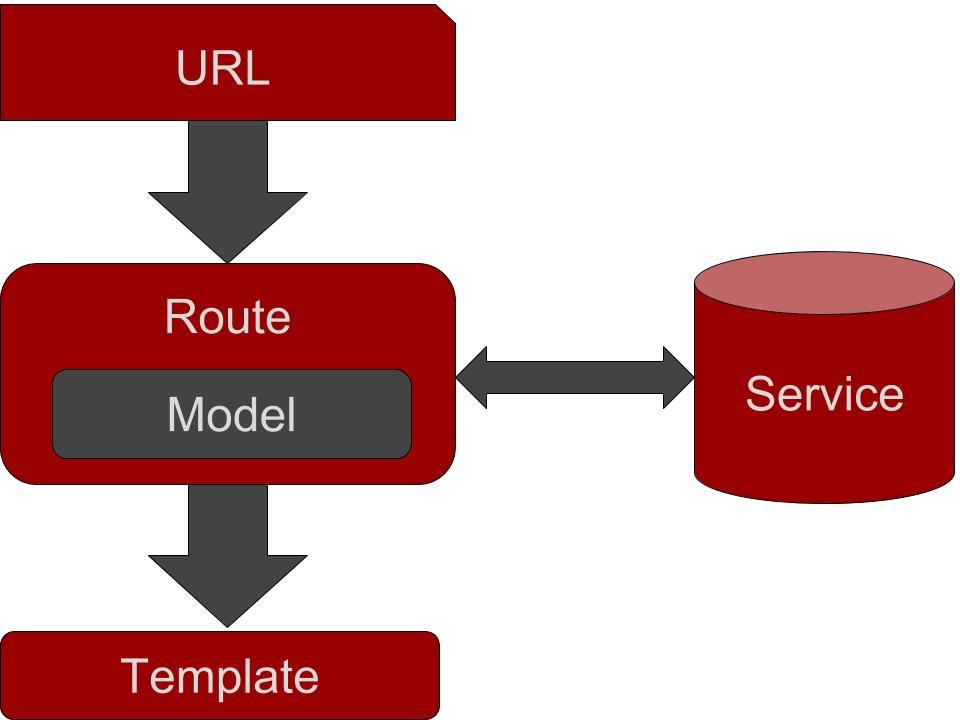
\includegraphics[width=\columnwidth]{figures/ember-programming-model}
\caption{Ember's Programming model}
\label{figure:ember-programming-model}
\end{figure}




Another framework that follows in the footsteps of Angular is EmberJS \cite{ember}. Just like every other MVVM framework, Ember also tries to achieve code minimalism by freeing the application developer from unnecessary boilerplate code and by utilizing declarative code when that seems fit. This framework adopts the action-page programming model, but since it's a client-side framework the entire action-page cycle takes place on the client. Ember's ecosystem comprises Routes, Models, Templates and Services. As shown in Figure \ref{figure:ember-programming-model} Ember's life-cycle starts when the user navigates to a URL that is bound to a particular Route. When the Route receives the event it generates the Model and calls the appropriate renderer that will generate the visual layer of the application. The Route can also utilize the appropriate reusable Services to receive essential data for the construction of the Model (application state).

Ember uses regular expressions to bind a Route to a particular URL. These expressions can also treat parts of the URL as variables, which enables message passing to and from other Routes. As we mentioned earlier Routes are responsible for constructing the Model of the application. Unlike Angular's Model which comprises Plain Old JavaScript Objects, Ember requires the extension of its internal Model objects. This is performed in order to enable efficient message passing between Model objects (as we will mention later), but it has a negative impact on the user friendliness, since the application developer needs to familiarize himself with the internal data structures used by Ember and the respective API that will be used to interact with them, which steepens the learning curve of the framework. Ember Routes are also able to utilize Services whose main goal is to assist in data transfer between local and remote databases and web services (Similar to Angular's Factories and Services).


\eat{
When a particular regular expression matches a URL, the respective Route will construct the Model by accessing a Service. The objective of Services is fairly similar to Angular's Factories and Services, their main goal is to assist in data transfer between local and remote databases and web services. After the appropriate dataset has been received from the Route, it has to construct the Model that is necessary for the next page that will be displayed. Unlike Angular's Model which comprises Plain Old JavaScript Objects, Ember requires the extension of its internal Model objects. This is performed in order to enable efficient message passing between Model objects (as we will mention later), but it has a negative impact on the user friendliness, since the application developer needs to familiarize himself with the internal data structures used by Ember, which steepens the learning curve of the framework.
}

EmberJS does not have its own custom template language, it instead utilizes a third-party template language called, HandlebarsJS \cite{handlebars} to generate the templates. Ember enables component wrapping by providing expendable Components (that are very similar to Angular's Directives). When importing such components the application developer can declaratively pass the Model that will be utilized by the component to generate (or update) the component specific view. Furthermore Ember provides modules that are very similar to Angular's Watchers, namely: Computed properties and Observable classes. These modules are used to listen for changes on the Model and cause the appropriate modifications on the application state. Computed values are mostly used when properties of the Model need to be composed by one or more other basic observable properties. When the computed property is initiated and one of the observable properties are updated, the computed property will be updated as well. Observable classes are mostly used to specify behaviors that will take place when the observable part of the Model changes. The application developer needs to provide a callback function, which most of the times contains imperative logic, in order to specify the respective behavior. 



\textbf{Accessors}

As we mentioned earlier Ember requires the usage of its internal object to represent the Model of the application. Particularly the application developer utilizes getters and setters when he wishes to retrieve and update the value of some Model variable. When the application developer sets a new value to some Model object an event triggers all the respective getters that are associated with that variable and causes them to re-evaluate the returned value. By doing so the application keeps the Model in sync at all times, without wasting resources by iterating over all the watched variables.





\eat{

\begin{figure}
\begin{code}
\directive{template}{delivery-trucks (product_name)}
 \directive{import}{functions}
 \directive{import}{actions}

 \textbf{<\% refresh} delivery_trucks =
     SELECT latitude, longitude, VIN, driver, 
            shift_start_time, avg_speed, 
            delivered_items, total_items
     FROM   delivery_trucks_table dtt, 
            product_delivery_truck_relation r, 
            products p
     WHERE  p.name = \directive{print}{product_name} 
            AND dtt.id = r.t_id AND p.id = r.p_id
 \textbf{\%>}
 \directive{html}{}
   <div>
     \directive{unit}{Google-Maps}
     \{
       options : \{
         zoom: 10,
         center: \{
           lat: -25.363882,
           lng : 131.044922
         \},
       \},
       markers : [ 
         \directive{for}{truck \textbf{in} delivery_trucks}
         \{
           position : \{
             lat : \directive{print}{truck.latitude},
             lng : \directive{print}{truck.longitude}
           \}      
         \}
       ]
     \}
     \directive{end unit}{}
   </div>
   <div>
     <table>
       <tr> <!-- ... column labels ... --> </tr>
       \directive{for}{truck \textbf{in} delivery-trucks}
          <tr>
            <td> \directive{print}{truck.VIN} /td>
            <td> \directive{print}{truck.driver} /td>
            <td> \directive{print}{truck.shift_start_time} /td>
            <td> \directive{print}{truck.avg_speed} /td>
            <td> 
               \directive{unit}{ProgressBar} 
               \{
                 type = 'Circle',
                 strokeWidth: 10,
                 trailWidth: 1,
                 easing: 'easeInOut',
                 from: \{ color: '#FC5B3F', width: 1 \},
                 to: \{ color: '#6FD57F', width: 10 \},
                 value : \{
                  numerator :\directive{print}{truck.delivered_items}
                  denominator : \directive{print}{truck.total_items}
                 \}
                \}
                \directive{end unit}{}
            </td>
          </tr>
         \directive{end for}{}
     </table>
   </div>
 \directive{end html}{}
\directive{end template}{}
\end{code}
\caption{Template \texttt{Delivery-Trucks}}
\label{figure:running-example:delivery_trucks-template}
\end{figure}
}

}

\eat{

\subsection{AngularJS}
\yannisk{This section includes for now a detailed comparison to AngularJS meant for our own understanding of the framework. Once it is ready, we will abstract out the important information and move it to the MVVM framework discussion above and/or to the complexity analysis} \yannisk{Costa, please use the command `projname' instead of `FORWARD' to refer to the framework's name.}

AngularJS (or simply Angular) is an open-source client side web application framework that has gained in popularity over the past few years. Angular is mainly maintained by Google but it has a big community of contributors and it has been used by multiple application developers throughout the globe. A simple search on StackOverflow will return over 120,000 results and a similar search on GitHub will return more than 88,000 repositories that have utilized AngularJS.

Angular's programming model has several similarities to FORWARD's. An AngularJS application is mainly comprised of \textit{Templates}, \textit{functions} and \textit{variables}. Within an AngularJS \textit{Template} the application developer utilizes Angular's template language to specify an abstraction of the view. Angular's template language contains pure HTML along with custom HTML tags and attributes which constitute an extension over the standard HTML directives, these are called Angular Directives. Angular's \textit{templates} just like FORWARD's contain bindings with \textit{variables} and \textit{function}. These bindings act as place-holders. During, run-time the variables and actions get evaluated and linked to the template thus generating a view on the browser. 


When events are triggered in an Angular application, they may cause side effects on the data model (variables and functions). When such changes occur Angular reflects them to the view. A big distinction from FORWARD is the fact that in Angular this happens automatically, there is no concept of manual action-page cycle, therefore the application developer has no controller over when do the changes get reflected to the view. Additionally if there are more than one sub-templates the application developer cannot choose the ones he wants to update, all of them will be updated. This can be extremely inefficient since in modern Angular applications a developer can choose to hide some sub-templates from the view (by using the css property "display:none"), if this is the case and a variable that is bound to several hidden sub-templates changes, angular will proceed to modify all the hidden sub-templates, even though the user will not be able to witness those changes.

\subsubsection{Angular's Digest Cycle}
Even though angular does not have the concept of a manual action-page cycle, it still manages to reflect changes of the model to the visual layer, and the way it accomplishes this with is called \textit{digest cycle}. 

}

\section{Conclusion}
\label{section:conclusion}

We presented \projname\ an interactive notebook engine, that enhances interactive notebooks with capabilities that pertain to both data scientist that create notebooks and non-technical notebook readers....

%\section{Introduction}
\label{section:introduction}

\noindent \textbf{Contributions} We describe the following contributions of \projname:
\begin{compact_item}

%

\item \textit{Declarative Semantics:} We present a formal declarative MVVM semantics for \projname. To the best of our knowledge, this is the first formal presentation of MVVM declarative semantics by an MVVM framework. \yannis{What extra do we offer in light of CIDR11 to the semantics?} 
\costas{Fundamentally, they are both diff driven application frameworks... Some differences are that the CIDR11 and SIGMOD10 version: 1.the template language was written in XML which was more verbose and therefore needed more effort to be written (more characters per line and more total lines of code for the same template instance). 2.Additionally, since template functions were not supported, the app developer often had to inline complex SQL++ queries in the template to ``massage" the data appropriately. 3. Delta functions were not supported. Overall templates appeared more convoluted compared to the current version and therefore they were harder to follow. For more differences check respective file in Notes folder (at the root of the repo)} \yannis{A large difference between CIDR11 and current work is the aim to easily interface with JavaScript. This is behind the functions in the template language, the interfacing of JavaScript components, the JavaScript actions and (the missing) easy programming model for accessing JavaScript data (the latter can stay for journal or OOPSLA)} Hence, the declarative semantics of \projname\ can also serve as an introduction to the semantics of MVVM at large, and to the semantics of \angular\ and other MVVM frameworks, after one accounts for their limitations.
%
\item \textit{Expressive Template Language:} While we draw from prior database research work, which treats the page as a database view, the template language goes beyond SQL query and view definitions in both style and fundamental expressiveness \yannis{Good point for a journal publication but on VLDB suffers from CIDR comparisons. The reason behind the higher expressiveness is new.}: It is a mixture of query language and web templating language that works on ordered data (arrays) and semi-structured data (JSON) \costas{JSON encompasses the concept of arrays/ ordered data}and is expressive enough to cover many common transformations without requiring the use of additional imperative JavaScript code. Notably, it is more expressive than the language of \angular, due to reasons pertaining to differences in their incremental rendering algorithms. \yannis{Cannot be quickly backed up by the example. Two nested loops may be hard but a for/if combo is doable.} \costas{How would it be backed up by example? We would have to introduce Angular and \projname\ templates in the intro, wouldn't we?} Furthermore, besides visualization, the templates can also input data and catch events/activate actions \costas{actions have not been defined}, as a complete web application development framework should do.

%
\item \textit{Incremental Rendering:} The incremental rendering problem has similarities to Incremental View Maintenance (IVM) but also poses distinct new challenges due to (1) template language features that have not received attention by the database community, and (2) unlike IVM whose goal is to update a target materialized view, the incremental rendering algorithm is a \textit{diff propagation} algorithm that results into a sequence of calls to the rendering methods of (the usually 3rd party) components. \yannis{A diff and its resulting rendering method call should have been demonstrated in the context of the example.} Pertaining to Item~(1) \projname\ solves the following diff propagation problems:
\begin{compact_enum}
\item \textit{Handling Arrays:} Arrays are prime citizens of the data model. Therefore we reconsidered what is the appropriate language for describing diffs, so that diffs on arrays are included. \costas{What do we mean when we say ``language" for describing diffs}\yannis{Current example has no motivation for insertion in the middle of array, which is where problems happen.}Second we developed algorithms for propagating such diffs.   
%


\item \textit{Black-box functions in Template:}\yannis{no example of a function either. It need not be the first example but I think there is just no example.} In the rare cases where the out-of-the-box expresiveness of the template language is not enough, the developer can include Javascript function invocations in her template. \projname\ offers a pay-as-you-go approach to the efficient diff propagation through JavaScript functions that may be part of the template: The developer may provide nothing (but the function itself), in which case the diff propagation algorithm will still work but may be slow\costas{Let's avoid the word slow, let's just say it wouldn't work ``incrementally", which is the more efficient.}, as it will be re-evaluating the function. Alternately, the developer may provide one or more diff management functions, which are suggested to her by \projname\ and lead to more efficient diff propagation. \costas{We should also mention that we provide some of these functions out-of-the-box (e.g sortby, groupby etc...)}\yannis{IMPORTANT: we need to discuss how this differs from angular's pay-as-you-go} \costas{Angular does not provide something similar to \projname's delta functions, so there's nothing to pay as you go}
%\costas{The IVM algorithm will be fast, the function re-evaluation may be slow (We should make it clear to the reader that the bottleneck isn't the template IVM algorithm but the user defined function...). That's why we enable the function developer to provide auxiliary delta functions that update the logical page more efficiently. }
%

\item \textit{Loops in Templates} \projname\ provides diff propagation over loop structures.  \costas{Why is that a big deal? This bullet doesn't illustrate why that's challenging or interesting...}\yannis{would be far more convincing with fors and ifs}

% 
\end{compact_enum}
%
The \projname\ incremental rendering also solves the following problems pertaining to its need to translate diffs into rendering method calls. \yannis{as said above, problems should have memorable names and do not repeat the whole description continously} \costas{refer to dictionary spreadsheet} \url{https://docs.google.com/spreadsheets/d/1pn6EPZUnz\_3Tc3e7FnveRxQXcs2uRqD0znERjI0-g0o/edit#gid=0}
\begin{compact_enum}

\item \textit{Easy wrapping of 3rd party components} A novel triggering algorithm enables the easy and pay-as-you-go wrapping of Javascript visualization rendering methods. In particular, the developer in charge of wrapping a visualization component is only tasked with specifying the single diff that a rendering method handles. \costas{This sentence doesn't make sense: ``(The developer specifies the) single diff that a rendering method handles". The developer does not specify diffs, he specifies renderer wrappers and diff signatures (refer to dictionary). The number of renderer wrappers he needs to specify is anything between two (construct-destruct) and the total number of renderers supported by the visualization library} \yannis{Needs example. Recall, earlier we introduced a diff and a corresponding renderer. Here we should change the assumption on renderer or the diff so that we can show simulation.}Therefore the size of the specification \costas{what specification?}is proportional to the number of rendering methods she wishes to wrap, as opposed to the number of the possible kinds of diffs, which is typically far larger. \costas{the latter number is: supported-diff opcodes X potential targets in unit instance} \yannis{tell the number that shows how many diffs exist in our example. You don't have to substantiate yet why so many. The substantiation will come much later once we have shown the unit's "schema" and have explained how many kinds of diff exist.
The most impressive introductions say "without my technique it would be N and with my technique it is M that is an order of magnitude below"} \costas{I don't follow. Why do we need to specify the number of possible diffs. When reading this section it feels like we're comparing our system with a system similar to ours that does not support simulation. Angular does not work with diffs, so this is somewhat pointless.} When a diff is produced that does not correspond directly to a rendering method, \projname\ discovers how to indirectly support it by \textit{simulating} the missing rendering method with existing wrapped rendering methods. \costas{we should add something like: ``This automation significantly simplifies the process of unit wrapping. Since competing frameworks do not provide a similar feature, unit developers are often required to manually perform it manually. This negatively impacts both the amount of time that needs to be spent in unit wrapping and the amount of lines of code that need to be written"}Lines-of-code experiments show the advantage of \projname\ in 3rd party wrapping productivity.

\eat{
\costas{The reasons why Angular directives need more lines are:
Actually the problem, arises when two renderers exist, one at a deeper level then the other. In such cases, Angular directive developers have to install a deep watcher at the higher level and manually compare the parts that correspond to more ``specific" renderers, to identify what changed. This happens to avoid the invocation of multiple renderers, which would be a direct result of}
}
%
\item \textit{Managing Direct Updates and Provenance Heterogeneity} \projname\ treats update diffs as first-class citizens, as opposed to simulating updates by insert-delete combinations. \costas{Not sure why we mention this, Angular directives don't need to simulate updates diffs with insert-delete diffs. Is this something that other IVM algorithms do not support?} This feature leads to higher performance and also superior UI behavior, when the visualization components provide update renderer methods. It also creates a need for keeping track of the provenance of each part of the visualization, so that it can be identified and updated. Notice that provenance has to be converted into terms that the 3rd party component understands, creating a need for special conversion data structures and algorithms. \yannis{Needs support of the example, both on the update and on the provenance. (The current example is an insertion and does not have any provenance problem.)}
\end{compact_enum}
%
\item \textit{Superior performance over other MVVM frameworks:} A net effect of the algorithms is that the client-side incremental rendering algorithm achieves better Big-O algorithmic complexity than the incremental rendering algorithm of \angular\ and also ouperforms it in the presented experiments.
%
\end{compact_item}

{\bf Paper Outline.} \yannisk{Revise after the sections have been finalized} The paper is structured as follows: In Section \ref{section:programming-model} we explain the structure of a \projname\ application as seen by an application developer. Section \ref{section:architecture} describes \projname's internal architecture, while Sections \ref{section:template-ivm}-\ref{section:visual-ivm} describe the incremental view maintenance algorithms that power the framework. Section \ref{section:experiments} compares the performance and productivity gains of the proposed system against the state of the art. Finally, Sections \ref{section:related-work} and \ref{section:conclusion} discuss related work and conclude the paper, respectively.
%\section{\projname\ Application Development}
\label{section:programming-model}

\yannisk{This section is currently disconnected from the introduction. After we decide on the main contributions in the introduction, we should connect it with the introduction.}  We present the structure and semantics of a \projname\ application as seen by its application developer. The internal execution of the application by the framework, along with the automatically applied optimizations, is the topic of Section \ref{section:architecture}. \yannis{There are two kinds of developers: The database-oriented developer and the JS developer. A JS developer can be an application developer. Hence, this is not the defining difference.} \\ 

\noindent \textbf{Running example.} We show how a developer can use \projname\ to create a temperature monitoring dashboard. The dashboard, shown in Figure~\ref{figure:running-example:screenshot}, consists of a chart showing the temperature readings as they arrive from a backend database. \yannisk{We should be careful how we describe the source of the new readings} The readings are represented by data points that are color-coded according to their value: Normal temperatures are shown in yellow, while lower and higher temperatures are shown with gradients of green and red, respectively. The normal temperature can be set by the user by utilizing the slider shown on the right side of the chart. %\yannis{I added ``range". Correct?}

The dashboard uses a combination of visualization components, allowing us to demonstrate how \projname\ interfaces with complex visualization libraries. In particular, the application employs two visualization components; a HighCharts component~\footnote{\texttt{http://www.highcharts.com/}}, displaying the chart and a Slider component for setting the normal temperature. \yannisk{Should we explain that we build the slider component in house? I vote for now, as it may raise questions.} \costas{We could say that we've wrapped all input types (see table: "Attribute Values" in: http://tinyurl.com/h5ktgqa) into units but it still does not explain why the range is color coded...}\\

\costas{Running example will be replaced. Revisit similar issues after it's finalized}


% Programming model figure
\begin{figure}[t]
\centering
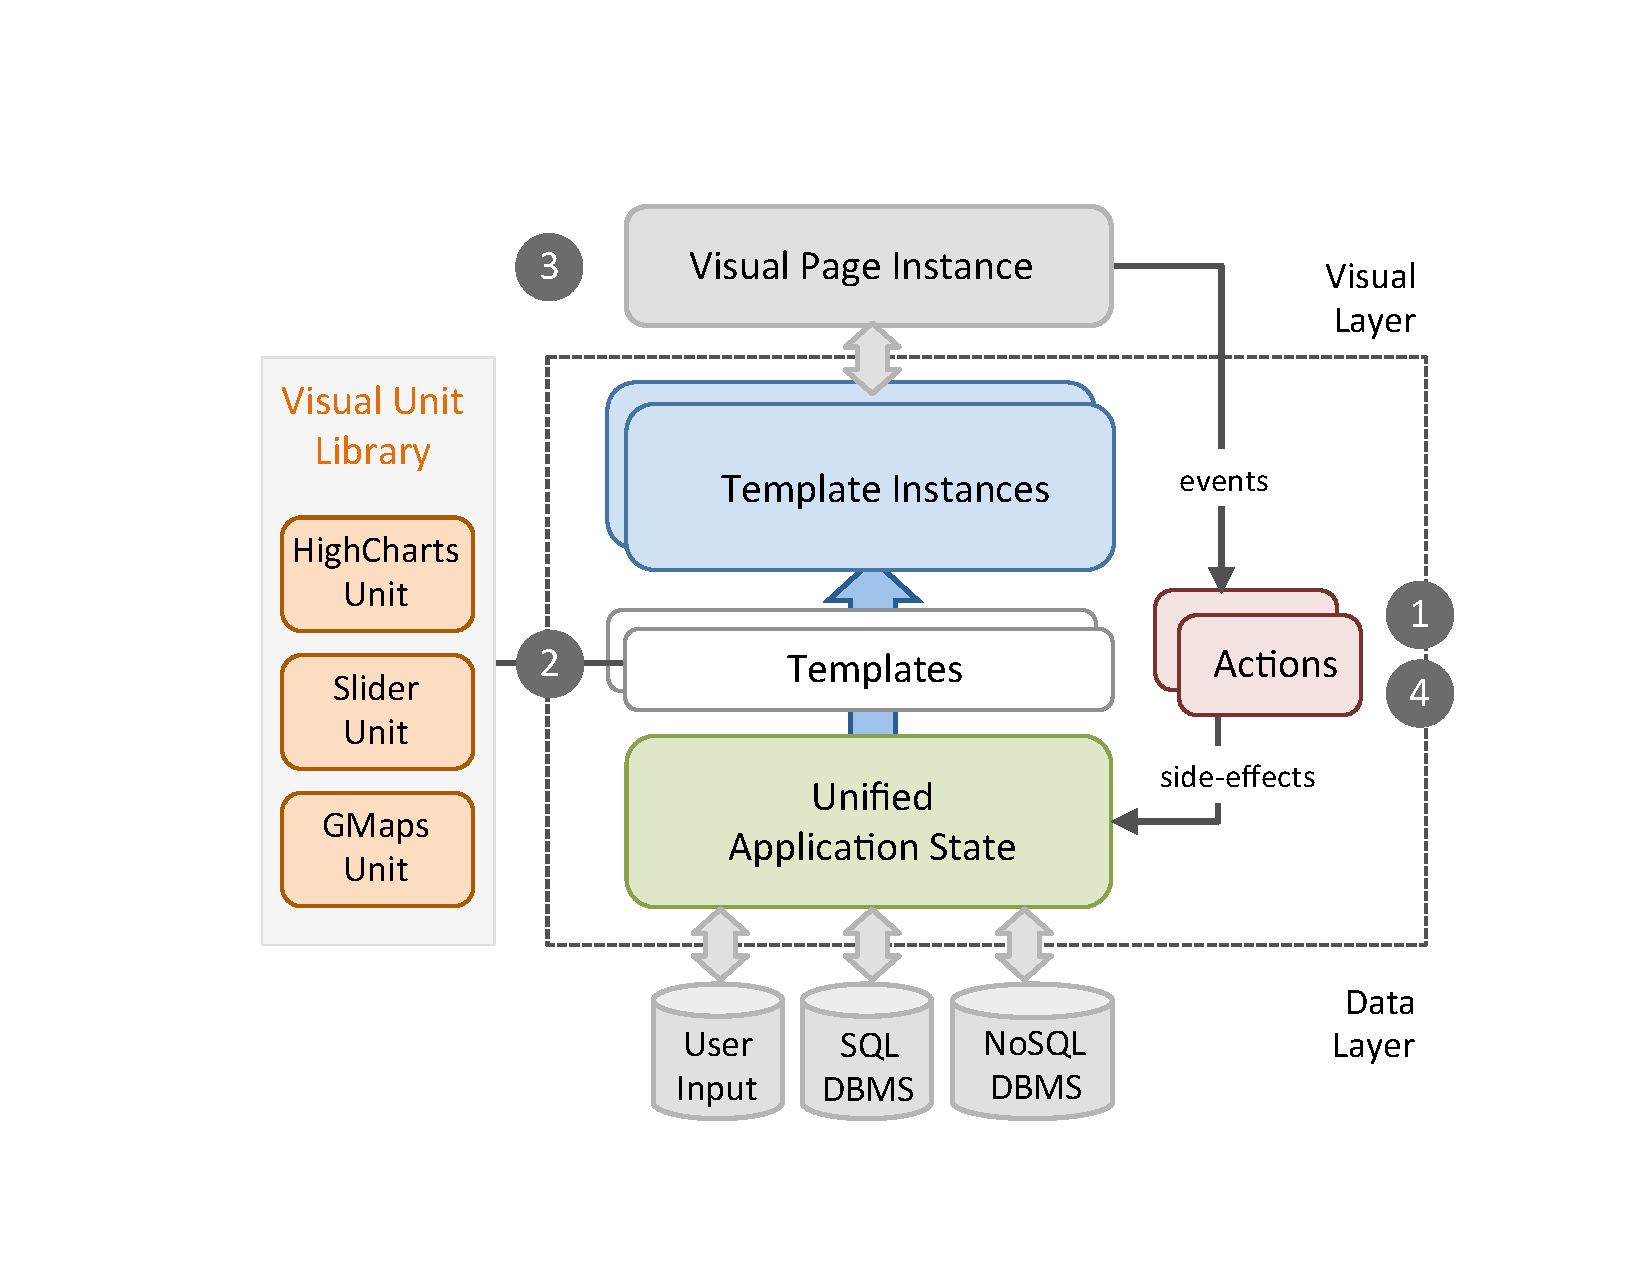
\includegraphics[width=\columnwidth]{figures/programming-model.pdf}
\caption{Programming model for an application developer. Actions, templates and UAS specifications are the pieces that are provided by the developer.}
\label{figure:programming-model}
\end{figure}


\yannis{About Figure: \ref{figure:programming-model}: instead of a virtual database we can go for just a series of active wrappers ("active" in the sense that they catch modifications)}

\yannis{There are two kinds of developers and the introduction never made the distinction: A db-oriented developer, who relies on the expressiveness of templates, and a Javascript developer who can write code, writes functions, interfaces components, writes complex actions. The distinctions need to become clear because some contributions pertain to the second kind of the developer. } \costas{I disagree with this distinction. Both developers need to write actions (in JS) in order to handle events. However, I do buy the argument that a naive application developer may not be able to write his own (delta) functions. Perhaps we should introduce the ``template function developer" (that makes reusable template functions) or simply mention that any ``advanced developer" can do everything a naive application developer does plus unit wrapping, (delta) function declaration and perhaps source wrapper declaration}

\textbf{Application structure.} Figure~\ref{figure:programming-model} shows the conceptual, developer-oriented architecture of a \projname\ application. It consists of:
(a) a \textit{unified application state (UAS)}\yannis{See above...}, abstracting access to the data sources that the application uses (e.g., the sensor readings in our running example), (b) \textit{template instances}, which abstract the structure of the \textit{visual pages} that are shown in the browser (e.g., describing in our running example the data points that will be shown and the visualization libraries that will be used to display them), %\yannis{Figure~\ref{figure:programming-model} should say ``Template Instances" in plural and use the ``multiple overlaid" boxes visualization that is used for Actions. But with blue color.}
(c) declarative \textit{templates}, specifying how the data in the UAS are transformed to template instances,
%\yannis{Figure~\ref{figure:programming-model} should say plural ``templates" and have a corresponding visualization.}
and (d) \textit{actions}, specifying the procedures that should be executed in response to events. The procedures may decide which template should be displayed and they may modify the UAS. 

During the runtime, an application follows an \textit{action-template cycle} in which actions activate templates that produce visual page instances. As new events occur they trigger respective actions again thus restarting this cycle. In particular, an action-template cycle consists of the following steps (denoted by numbers in Figure~\ref{figure:programming-model}): %First, the data used by the application (step 1) are abstracted as a virtual database (UAS) instance (step 2). 
%\yannis{The fact that we associate template-action cycle steps with the abstraction gives the damaging impression that there is actual computation involved in going from source data to UAS. I have changed the text to remove this impression but you need to remove the steps 1 and 2 from Figure~\ref{figure:programming-model}.}
An action is activated (step~1) and chooses the template that will be displayed. At that time the action can also cause side-effects to the application state by interacting with the UAS instance. 
Subsequently, \projname\ evaluates the chosen declarative template on the UAS (step 2), which produces an abstraction of the visual page in the form of a template instance. Then \projname\ automatically produces a new visual page instance from the template instance (step 3). Finally, user interface events are caused as the user interacts with the visual page instance, thus triggering actions (step 4), that lead to repetition of the action-template cycle. We next describe each of the pieces of a \projname\ application in detail. \costas{It is possible for an action to not trigger a template (for instance an action could simply collect data from the page and store them locally or transmit them over-the-wire to a remote source)}

%Figure \ref{???}a, b, and c shows the virtual database, template and template instance for our running example, respectively. We next describe each of these components in detail.\\

% Template and template instance figures
\begin{figure*}
\centering
%
\begin{minipage}[c]{8.5cm}
\begin{code}
\directive{template}{temp\_view()}
  \directive{import}{functions}
  \directive{import}{actions}

  \textbf{<\% let} readings = select t.temp
                    from db.temperature as t
                    order by timestamp \textbf{\%>}
  
  \directive{unit}{highcharts}
  \{\eat{
    chart: \{
      renderTo: 'container',
      zoomType: 'x'
    \},}
    title: \{ text: 'Temperature monitor' \}, \eat{
    plotOptions: \{
      series: \{
        turboThreshold: 5000000
      \}
    \},
    subtitle: \{
      text: 'Using the experimental Highcharts Boost module'
    \},
    tooltip: \{
      valueDecimals: 1
    \},}    
    series: [\{
      data: [
        \directive{for}{reading \textbf{in} readings}
          \{
            y    : \directive{print}{reading.temp},
            color: \directive{print}{toHex(reading.temp, threshold)}
          \}
        \directive{end for}{}
      ],
      lineWidth: 1
    \}],
    \gl{<\% event} onSelection redrawSelected() \gl{\%>}
  \}
  \directive{end unit}{}
  
  \directive{unit}{slider}
  \{
    min  : 0,
    max  : 10000,
    value: \directive{bind}{threshold = 65}
  \}
  \directive{end unit}{}
\directive{end template}{}
\end{code}
\vspace*{-0.3cm}
\subcaption{Template \texttt{temp\_view}}
\vspace*{0.3cm}
\label{figure:running-example:main-template}
\end{minipage}
%
\hspace{1cm}
%
\begin{minipage}[c]{6cm}
%
\begin{minipage}[c]{6cm}
\begin{code}
\directive{unit}{highcharts}
\{\eat{
  chart: \{
    renderTo: 'container',
    zoomType: 'x'
  \},}
  title: \{ text: 'Temperature monitor' \},\eat{
  plotOptions: \{
    series: \{
      turboThreshold: 5000000
    \}
  \},
  subtitle: \{
    text: 'Using the experimental Highcharts Boost module'
  \},
  tooltip: \{
    valueDecimals: 1
  \},}    
  series: [\{
    data: [
        \{ y: 55, color: '#359435' \},
        \{ y: 57, color: '#359823' \},
        \{ y: 56, color: '#359533' \},
        \{ y: 53, color: '#359220' \}
    ],
    lineWidth: 1
  \}]
\}
\directive{end unit}{}

\directive{unit}{slider}
\{
  min : 0,
  max : 10000,
  value: 65
\}
\directive{end unit}{}
\end{code}
\vspace*{-0.3cm}
\subcaption{Template instance}
\label{figure:running-example:main-template-instance}
\vspace*{0.3cm}
\end{minipage}
\begin{minipage}[c]{6cm}
\begin{code}
   sources : [ \{ 
     driver   : "postgres", 
     host     : "localhost", 
     port     : 5432, 
     aliases  : [\{db : "sensorDb"\}]
     username : "dbadmin" 
   \}] 
\end{code}
\subcaption{UAS configuration file}
\label{figure:uas-config-file}
\end{minipage}


%
\end{minipage}
\caption{Template, template instance, and UAS configuration file for the running example}
\end{figure*}

% Lines of different concepts in the template and template instances
\newcommand{\templateinstanceline}[1]{%
    \IfEqCase*{#1}{%
    {highcharts-unit-instance}{lines~1-14}%
    {slider-unit-instance}{lines~16-22}%
    }[\errmessage{Unable to ref #1 for template instance}]%
}%

\newcommand{\templateline}[1]{%
    \IfEqCase*{#1}{%
    {highcharts-unit}{lines~9-24}%
    {slider-unit}{lines~26-32}%    
    {print-y}{line~16}%
    {print-color}{line~17}%
    {for}{lines~14-19}%
    {let}{lines~6-8}%
    {bind}{line~30}%
    }[\errmessage{Unable to ref #1 for template}]%
}%

\yannis{About Figure \ref{figure:running-example:main-template}: Why the importing is on the template? The actions may not be template specific. Same for the functions.}

\costas{Yes, the template needs to be changed.}

\yannis{About Figure \ref{figure:running-example:main-template}: The total absence of html and/or any form of unit testing hurts the idea that we do pages. }

\costas{The two units should be wrapped by an HTML unit. I believe this was done like that to avoid an extensive description on fragmentation.}

\yannis{About Figure \ref{figure:running-example:main-template}: The query suspiciously lacks any window }

\costas{The application shows historic data, it doesn't show a particular window. The user however can use the chart to zoom into some time window, to explore the data.}

\yannis{About Figure \ref{figure:running-example:main-template}: Query almost covers the provenance heterogeneity problem behind time stamp.}

\yannis{About Figure \ref{figure:running-example:main-template-instance} slider unit: May be good to have a non-initial value and talk about it.}

\subsection{Unified Application State (UAS)}
\label{section:vdb}

%\textbf{Abstracting out application data through a virtual database.}
Modern web applications retrieve data from a variety of sources, including backend databases (both SQL and NoSQL), browser storage (such as IndexedDB), web services and user input (through forms). \projname\ abstracts all data sources into a \emph{unified application state} (in short \emph{UAS}), which serves two purposes: First, it provides unified distributed accesses to multiple sources, in the spirit of virtual databases. Second, it efficiently observes modifications to data sources, which is an important step to \projname's incremental computation ability and a major topic of this paper. A UAS instance is a tuple of the form $\langle x_1 : v_1, \ldots, x_n : v_n \rangle$, where each $x_i$ is a variable bound to the value $v_i$.

\costas{The UAS instance corresponds to the (Client-Side) Application Model}

\yannis{if we abolish the UAS and go with the functions approach, this section says that the results of the functions are JSON++
TBD whether we need functions that also input JSON++. If we do, then it can be the template language itself. It only lacks recursion. At any rate it is probably journal version material.}

UAS values are represented through the JSON++ data model: an extension of the (common in web applications) JSON data model with support for unordered collections (bags). This extension is crucial to support  propagation of changes that happen to bags of tuples (typically produced by relational DBMSs) as we will see in Section \ref{section:template-ivm}. A JSON++ value can be a scalar (i.e., string, number or boolean), tuple of attribute/value pairs, array of values (i.e., ordered collections), or bag of values (i.e., unordered collections). \costas{Since bags and JSON tuples inherently use keys, perhaps they can be both encoded as tuples thus simplifying the data model that has to be understood by unit developers - Note, we agreed to do it this way during our last meeting.} Complex values (i.e., tuples, arrays, and bags) recursively contain other JSON++ values, thus allowing the representation of nested data. Finally, internally each value may also contain a \textit{provenance annotation} (in short \emph{provenance}), which is leveraged by the change propagation algorithm. Note, the application developer need not be aware of it. 
\eat{A provenance annotation is required for all values of a bag and is optional otherwise. \yannisk{The presence of ids does not have to do with the type of the JSON++ value. Instead it has to do with the type of diffs that the source can produce. For instance, in our running example the output of the SQL query is an array (since the query uses an order by clause), but the elements of the array should still contains ids, since relational IVM solutions cannot produce diffs that use ordinals.} \yannisk{The framework is currently missing a few features for the full support of ids. In particular: (a) Since bag elements should contain ids, the application developer should specify whenever she creates a bag in the template how the ids of its elements will be populated. Similarly, for the result of SQL queries. Any ideas on how to do that? (b) With the inclusion of ids in arrays, a single diff can be represented in two different ways (through an id or through an ordinal). Thus simulation should be extended to handle this case as well. (c) How are JSON++ values physically represented? Are they encoded in JSON?} 
}

The following table shows the notation used to represent the different types of JSON++ values:\\

\noindent\begin{tabular}{@{}l | l}
JSON++ Value & Type
\\ \hline
``string'' | x | true/false & Scalar (string/number/boolean)
\\
$\langle x_1 : v_1, \ldots, x_n : v_n \rangle$ & Tuple of attribute/value pairs
\\
$[ v_1, \ldots, v_n ]$ & Array of values
\\
$\{\!\{ v_1, \ldots, v_n \}\!\}$ & Bag of values
\\
$\#(k_1, \ldots k_n) \text{ }v$ & Value with provenance $(k_1, ..., k_n)$
\\
\end{tabular}
\vspace*{0.4cm}



To associate the UAS instance with data from a particular source, the developer has to specify the type of the source (e.g., SQL database) and, when applicable, provide the parameters required for connecting to the chosen source type (e.g., host and account information for the database server). This information has to be provided in the form of a UAS configuration file. For instance, Figure~\ref{figure:uas-config-file} shows the UAS configuration file for the running example. In the case of browser resident JSON++ objects, the developer simply needs to access them via the UAS interface. \yannis{Kosta, is the previous sentence fair?} \costas{Not really, you're probably talking about accessing variables of the client-side Model. The client-side Model is simply a collection of Plain Old JS Objects. This collection of variables is encompassed by the client-side (JavaScript) VDB/Model variable. Since they are all POJO's no API is required, the developer interacts with them as she would with any other JS Object. \eat{(If however we decide to use a different construct (other than POJSO) for bags we might have to introduce an API for accessing that)}}
As we will see in Section \ref{section:template}, the template may also introduce new variables to the UAS. Some of these variables are associated with derived data (i.e., they are tantamount to database views) and some other ones are associated with page input. \yannisk{We should give more details on how the configuration file affects the UAS instance. We could extend the UAS instance to contain non-JSON++ values corresponding to sources (e.g., the instance may contain a variable \emph{db} corresponding to a relational database) but this breaks the nice abstraction that we want to create. Any ideas/suggestions?} \yannis{Don't we need to extend the JSON++ with arbitrary enriched types? Is string, number and boolean enough?}

\subsection{Template Instance}
\label{section:template-instance}

\begin{figure}[t]
\centering
%\scriptsize
\begin{tabular}{B}
\hline
 1  & \gn{template\_instance}   & \gp   & \gn{unit\_instance}                                       \\
 2  & \gn{unit\_instance}         & \gp   & \gl{<\% unit} \gn{unit\_class} \gl{\%>}               \\
    &                           &       & ~~ \gn{value}                                         \\
    &                           &       & \gl{<\% end unit \%>}                                 \\
 3  & \gn{value}                & \gp   & \gn{jsonpp\_value} %\text{(see Figure~\ref{figure:bnf-value})} 
 \\
 4  &                           & \gd   & \gn{unit\_instance}                              
\\ 
\hline
\end{tabular}
\caption{BNF Grammar for Template Instances}
\label{figure:bnf-template-instance}
\end{figure}

\eat{
\begin{figure}[t]
\begin{code}{B}
init() \{
   display(temp\_view);
\}
\end{code}
\caption{Initial action}
\label{figure:action}
\end{figure}
}



\yannisk{Double-check line numbers for all figures}

The main challenge at the visual layer is the variety of visualization libraries that may be used in a web application, along with the fact that tedious low-level programming is required to perform incremental rendering with the APIs provided by those libraries. Modern web applications commonly include a huge variety of visual components, such as charts, maps, and sliders, each with their own APIs.


\noindent \textbf{Visual Units} \yannis{Header "Visual Units"}

\noindent To shield developers from low-level programming, \projname\ abstracts out each visual component as a \projname\ \emph{visual unit} (or simply \emph{unit}). In the eyes of an application developer a visual unit is a black box that takes as input a JSON++ value \costas{I believe we mean JSON value here, I don't see why the application developer should learn about bags and why they are useful}containing the data to be visualized and parameters potentially supported by the visualization and uses the API of the underlying visualization library to render the visual component. As such a particular instantiation of the unit (denoted as \emph{visual unit instance} or simply \emph{unit instance}) can be described as $\gl{<\% unit } U \gl{ \%> } v \gl{ <\% end unit \%>}$, where $U$ the type of the visual unit and $v$ the JSON value corresponding to the input of the unit. For instance, \templateinstanceline{highcharts-unit-instance} of Figure \ref{figure:running-example:main-template-instance} show a unit instance of type \texttt{highcharts}. The unit instance specifies both the data that should be shown on the chart (as an array of tuples assigned to the \texttt{data} attribute) and the values of the parameters accepted by the unit (such as the chart's title).

\yannis{better to have HTML in the example but do not spend too much time on it in the abstract discussion}

As we will discuss in Section \ref{section:architecture}, visual units are generated by visual unit developers who wrap popular visualization libraries (such as Google Maps, HighCharts, etc) and make them available to application developers through \projname's visual unit library. In addition to the units provided by unit developers, \projname\ also provides a special unit of type \emph{HTML}. In contrast to other units, which expect JSON values, an HTML unit takes as input a sequence of HTML tags, allowing developers to easily create simple HTML content. For ease of exposition we focus in this paper on JSON units. Our results can be easily extended to the HTML unit. \costas{So far we've been talking about JSON++ if we keep that, we should make it clear why in this paragraph we only talk about JSON and HTML}\yannisk{Removed HTML unit encompassing the two JSON units from our running example}

%Yannis comments mentioned to delete the "eaten" sentence
\eat{Since a single visual component can be described through a unit instance, }An entire visual page instance (potentially containing multiple visual components) can be described through a composition of unit instances. We refer to this logical description of a visual page as \emph{template instance}, as it is not written directly by the developer but is instead the result of instantiating a \emph{template}, as we will see next. Figure \ref{figure:running-example:main-template-instance} shows a template instance for our running example. It consists of two unit instances; a highcharts unit instance (\templateinstanceline{highcharts-unit-instance}) and a slider unit instance (\templateinstanceline{slider-unit-instance}). Note that a unit instance may recursively contain nested unit instances \yannisk{Example?} \yannisk{What does it mean for a unit to be nested within another unit? Can we nest arbitrary units or only units that are designed as such by the unit developer?} \yannis{Arbitrary.} \costas{The child unit is Arbitrary. However, a child unit can only be attached at predefined locations of the parent unit (i.e When the parent unit is google maps, a child unit can only be attached under the infowindow location since that's the only attachment point that is supported by the Google Maps API)}
Figure \ref{figure:bnf-template-instance} shows the grammar for template instances. Finally, to simplify the architecture, template instances are internally represented as JSON++ values. This is achieved by encoding a list of unit instances $\gl{<\% unit } U_1 \gl{ \%> } v_1 \gl{ <\% end unit \%>}$ \ldots $\gl{<\% unit } U_n \gl{ \%> } v_n \gl{ <\% end unit \%>}$ as a JSON++ tuple \texttt{\{$U_1'$: $v_1$, \ldots, $U_n'$: $v_n$\}}, where $U_i'$ is a unique identifier assigned by \projname\ to the i-th unit instance. \yannisk{OK or too cryptic?}

\yannis{We need reserved keywords for the attribute names that correspond to units. Eg, \_\_myunit} \costas{How can we have a predifined set of reserved keywords given that there's an arbitrary number of possible units each with a unique name?}

%Based on this idea, \projname\ abstracts out the entire visual page in the form of a logical specification, referred to as a \emph{template instance}. The template instance contains a description of the visual units that should be displayed in the page together with their inputs. For instance, Figure \ref{???} shows the template instance of our running example. It consists of two unit instances, one of type HighCharts and one of type \ref{???}. Each unit instance is denoted as $\gl{<\% unit } U \gl{ \%> } v \gl{ <\% end unit \%>}$, where $U$ the type of the visual unit and $v$ the JSON value corresponding to the input of the unit. A special type of unit is an HTML unit for displaying HTML content. An HTML unit instance is of the form $\gl{<\% html \%> } e_1 \ldots e_n \gl{ <\% end html \%>}$, where $e_1, \ldots, e_n$ are HTML elements.

\subsection{Template}
\label{section:template}

\begin{figure}[t]
\centering
\scriptsize
\begin{tabular}{B}
\hline
 1  & \gn{template}             & \gp   & \gl{<\% template} \gn{template\_name} (\gn{param\_list}) \gl{\%>}                    \\
    &                           &       & ~~ \gn{let}*                                    \\
    &                           &       & ~~ \gn{unit}
\\
    &                           &       & \gl{<\% end template \%>}                                         \\
 2  & \gn{param\_list}			& \gp   & ( \gn{var\_name} (, \gn{var\_name})* )? 
\\ \hline
 3  & \gn{unit}         & \gp   & \gl{<\% unit} \gn{unit\_class} \gl{\%>}               \\
    &                           &       & ~~ \gn{value}                                         \\
    &                           &       & \gl{<\% end unit \%>}                                 \\
 4  & \gn{value}                & \gp   & \gn{jsonpp\_value} %\text{(see Figure~\ref{figure:bnf-value})} 
\\
 5  &                           & \gd   & \gn{unit}                                     
\\
 6  &                           & \gd   & \gn{print}                                                        \\
 7  &                           & \gd   & \gl{[} \gn{for} \gl{]}                                                                                \\
 8  &                           & \gd   & \gl{<} \gn{for} \gl{>}                                                                                \\
 9  &                           & \gd   & \gn{if}                                                                                 \\
  
 10  &                           & \gd   & \gn{bind}                                                         \\
11  &                           & \gd   & \gl{\{} \gn{event}*                                               \\
    &                           &       & ~~ (\gl{\textquotedbl}\gn{string}\gl{\textquotedbl} 
                                             \gl{:} \gn{value}                                              \\
    &                           &       & ~~ (\gl{,} \gl{\textquotedbl}\gn{string}\gl{\textquotedbl} 
                                             \gl{:} \gn{value})* )? \gl{\}}                                           \\ \hline
12  & \gn{let}                 & \gp   & \gl{<\% let} \gn{var\_name} \gl{=} \gn{expr} \gl{\%>}            
\\
13  & \gn{print}                & \gp   & \gl{<\% print} \gn{expr} \gl{\%>}                                 \\
14  & \gn{for}                  & \gp   & \gl{<\% for} \gn{var\_name} \gl{in} \gn{expr} \gl{\%>}           
\\
    &                           &       & ~~ \gn{let}*                                    \\
    &                           &       & ~~ \gn{value}
\\
    &                           &       & \gl{<\% end for \%>}                                              \\
    
14  & \gn{if}                  & \gp   & \gl{<\% if}  \gn{expr} \gl{\%>}           
\\
    &                           &       & ~~ \gn{value}
\\
 &                           &       & ~~ (\gl{<\% elif}  \gn{expr} \gl{\%>} 
 
\\
 &                           &       & ~~ \gn{value})*    
 \\
 &                           &       & ~~ (\gl{<\% else}  \gl{\%>} 
 
\\
 &                           &       & ~~ \gn{value})?    
\\
    &                           &       & \gl{<\% end if \%>}                                              \\
15  & \gn{bind}                 & \gp   & \gl{<\% bind} \gn{var\_name} = \gn{expr} \gl{\%>}                             \\
16  & \gn{event}                & \gp   & \gl{<\% event} \gn{event\_name} \gn{action\_name} \gl{\%>}        \\
17  & \gn{expr}                 & \gp   & \gn{js\_expression}                                               \\
18  &                           & \gd   & \gn{source\_expression}                                                   \\
19  &                           & \gd   & \gn{json\_path}                                                   \\
\hline
\end{tabular}
\caption{BNF Grammar for Templates}
\label{figure:bnf-template}
\end{figure}

\yannis{About Figure \ref{figure:bnf-template}: the syntax allows a single top level unit, which is probably correct but not what the example does.
Is the top level unit always html?}

\yannisk{To do: Modify template BNF grammar to make sure that we can have directives appear inside JSON values}
\emph{Templates} are declarative specifications describing the template instances as a function of UAS data. A template specifies this function through a set of \emph{template directives}, so that it provides syntax similar to well-known template languages, while it is essentially an expression of a functional programming language without recursion. A template also specifies collecting data from the page and catching events \costas{perhaps we mean linking event with corresponding actions?}. 

There are five template directives: \gl{<\% print \%>}, \gl{<\% for \%>}, \gl{<\% let \%>}, \gl{<\% bind \%>}, and \gl{<\% event \%>}. These are used to describe computation, define variables, set up data collection and specify events. We next describe each of them in detail.\\

%Figure \ref{???} shows for instance the template for the heat map view of our running example. As we will explain in Section \ref{section:templates}, the template language is expressive enough to cater for the needs of most visual units and pages encountered in practice, supporting among others iteration through for loops and function calls. An application may contain more then one templates, which can be displayed as the result of actions, discussed next.\\


\yannis{From an expressiveness point of view, let does not add anything. The interesting consideration is whether it has a meaning about IVM: materialized vs virtual intermediate result.}
\noindent {\bf Defining variables.} A template may define variables that are added to the UAS instance so that they can be used in subsequent computation. Variable definition is facilitated by the \gl{let} directive.

The $\gl{<\% let } x \gl{ = } E \gl{ \%>}$ directive defines variable $x$ in the UAS, and assigns to
$x$ the result of evaluating the expression $E$. The expression $E$ can be a JavaScript expression, a source-specific language (such as a SQL query in the case of relational database sources) or a JSON++ path. For example, the template of our running example (\templateline{let}) employs a \gl{let} directive to create a variable \texttt{readings} containing all temperature readings (retrieved from a relational DBMS through a SQL query).\\

{\bf Reporting syntax and semantics.} Computation in a template is specified using the \gl{print} and \gl{for} directives.
The $\gl{<\% for } x \gl{ in } E \gl{ \%> } B \gl{ <\% end for \%>}$ directive specifies that variable $x$ iterates over the result of the expression $E$. In each iteration, the body $B$ of the \gl{for} loop is instantiated. For example, the template of our running example (\templateline{for}) uses a \gl{for} directive to iterate over the sensor readings (stored in the \texttt{readings} variable). For each reading, it generates a new JSON tuple of the form \texttt{\{y:\ldots, color:\ldots\}}, which is the data format expected by the HighCharts unit for each data point. \eat{The values of the \texttt{y} and \texttt{color} attributes are specified through print directives, as explained below.}

% Eaten as per Yannis\' comment

The $\gl{<\% print } E \gl{ \%>}$ directive instantiates the result of expression $E$. For example, the template of the running example uses two \gl{print} directives to generate the values of the \texttt{y} and \texttt{color} attributes of each JSON tuple produced by the \gl{for} directive. \yannis{The part between the ``\{\}" could be removed}\{The value of \texttt{y} is created by printing the value of the \texttt{reading} variable (\templateline{print-y}), while the value of \texttt{color} is generated by calling the \texttt{toCSS} function, which takes as input the current reading and the normal temperature (set through the slider) and produces a CSS color code according to the coloring schema explained above (\templateline{print-color}).\}\\

%(Figure~\ref{figure:running-example:main-template}) generates the CSS color of a \texttt{<td>} element (i.e., of a table cell) by instantiating through a print directive the result of the \texttt{toCss()} function (which translates a value to a CSS color code according to the setting of the threshold).

%The $\gl{<\% refresh } y \gl{ = } E \gl{ \%>}$ directive defines \textit{derived variable} (i.e., a variable that is computed using one or more other variables) $y$ in the UAS, and sets $y$ to the result of expression $E$. The expression $E$ can be a JavaScript expression, a SQL query or a JSON++ path. For example, \yannisk{TBD}
%the heat map template (Figure~\ref{figure:running-example:main-template}) specifies a derived variable \texttt{matrix} for product stock data instantiated to the result of a SQL query.
%\yannisk{Why does the framework differentiate between base and derived variables?}\\ 

%An important distinction between base variables and derived variables is as follows. A view $Y$ is declaratively specified to be refreshed with the evaluation result of $E_Y$, thus enabling the \projname\ framework to utilize IVM optimizations for incrementally evaluating $E_Y$. In contrast, a base variable $X$ is imperatively updated using either \texttt{INSERT} / \texttt{UPDATE} / \texttt{DELETE} commands on the UAS, or user input through the bind directive (explained below), and therefore the \projname\ framework does not optimize these updates.\\

{\bf Collecting data.} In addition to specifying how to compute a template instance, the template's \gl{bind} directive allows the developer to specify how data are collected from user input on the page.

The $\gl{<\% bind } x = E \gl{ \%>}$ directive specifies that the template instance attribute value in whose position the directive appears will be assigned to variable $x$. This allows UAS variables to become bound to input received by visual units.  \yannis{If UAS has not been defined we need to say what is the JavaScript target.} \costas{We should define a Model/VDB variable, that encompasses every client-side variable used in an application. The target in this case would be the Model.x variable} For instance, the template of our running example (\templateline{bind}) uses a \gl{bind} directive to assign to variable \texttt{threshold} the current value of the slider (which is returned by the slider unit as the value of the \texttt{value} variable). The \gl{bind} directive also allows the developer to specify an expression $E$, whose value will be assigned to the variable when the template is first instantiated. For example, the slider of our running example is initialized with the value 65.\\

%In contrast to the \gl{<\% print \%>} directive, which is a one-way binding from the UAS to the visual instance, the \gl{<\% bind \%>} directive specifies a two-way binding between the UAS and the visual instance, thus allowing values to be collected from the visual interface. For instance, \yannisk{TBD}\\
%the heat map template (Figure~\ref{figure:running-example:main-template}) specifies that the value of the slider will be bound (i.e., assigned) to the \texttt{threshold} variable.\\

{\bf Specifying event handlers.} Finally, a template allows also the invocation of actions in response to events. The $\gl{<\% event } e \gl{ } a \gl{ \%>}$ directive specifies that whenever event $e$ of the enclosing unit instance occurs, action $a$ is executed. For instance, \yannisk{Costa, please add event to template and add description here.}\\
%the heat map template (Figure~\ref{figure:running-example:main-template}) specifies that whenever the position of the slider unit is changed, the action \texttt{updateThreshold} will be executed . \yannisk{Costa, what will this action do?} \yannisk{Do we assume that units come with predefined events?}\\

\costas{}

Finally, each template may also accept parameters that are passed to it by its caller by value. When the template is instantiated, \projname\ creates for each parameter an identical-named UAS variable and then sequentially scans the template instantiating its directives.

\subsection{Actions}
An action is a Javascript procedure that is invoked in response to events and can also read and write to the UAS, cause side-effects in external systems, such as charge a credit card through a REST service, and specify which template should be displayed next. In visualization applications, such as the running example, actions are very simple, since they only specify the next template to be instantiated. For example, see \yannis{Kosta, please put a super simple action.} \costas{Will do after we replace the running example} \costas{I think it makes sense to introduce a system-provided action (named redisplay\_template()), that simply redisplays the current template, when an event occurs. This would allow eager application view maintenance without requiring extra imperative code from the app developer.}

\eat{
The events that can cause the firing of an action may be initiated by the user (such as a user clicking a button) or an external process (such as a browser timer event fired every 30 seconds or the arrival of data from the server). An application developer can associate an event to an action through the the \gl{<\% event \%>} directive, explained above.
}

\subsection{Application Specification Summary}
\yannis{Could be shortened to one sentence at start}
To specify an application, the developer thus has to provide the following components: (a) a specification of the UAS describing how data from different sources are mapped into variables, (b) a set of templates describing how to transform the UAS to visual pages, and (c) a set of actions, describing how the application should react to events. \costas{(a) assumes that \projname\ is used as a full stack framework, perhaps we should also mention that if the developer wishes to only use \projname\ as a client-side framework, instead of (a) she has to simply provide the JSON objects that constitute the model. Additionally, when we describe the source wrappers it might make sense to introduce a REST/Websocket wrapper that works with 3rd party services. This wrapper would provide diffing capabilities without requiring the app developer to manually diff the model (this diffing would most likely have to take place on the client)}

%\yannisk{How do we explain that templates may also include variable definitions and data collection specification?}
%\yannisk{In case we describe other MVVM frameworks in the introduction, tie this section in with the introduction by explaining the correspondence between \projname\ and MVVM framework components.} 

%A \projname\ application comprises a \textit{virtual database} \costas{we've been using the term logical page in the previous sections we should bridge the gap by mentioning that this is the UAS} (or \textit{UAS}), \textit{templates} and \textit{actions}. Intuitively, \projname\ models an application as a state machine. (1) The UAS is an abstraction that represents the state across multiple data sources, such as SQL and NoSQL databases. (2) A template visualizes UAS state by instantiating a \textit{template instance}, which is an abstraction of multiple visualizations including HTML, heat maps, sliders and other JavaScript libraries. (3) An action causes state transitions by writing to the VDB.

%During runtime, each page of the application executes in an \textit{action-template} cycle as follows. An \textit{event}, such as the user clicking a button, invokes an action. In the running example, there are three events that invoke an action: (1) when the user first loads the page in the browser, (2) a timer event that fires every 30 seconds \costas{maybe we should replace this with an "event triggered by a new diff coming from the backend" triggers are more efficient than polling} \yannisk{I would suggest to stay with the polling, as allowing the arrival of diffs to also cause actions will complicate the picture we discussed, where the arrival of diffs is decoupled from the actions: diff arrivals simply cause IVM but do not have any effect on the action-template cycle} , and (3) when the user changes the threshold with the slider. An action specifies a procedure that reads and writes the VDB, and causes side-effects in external systems such as charging a credit card through REST services. Typically, the last step of the procedure enqueues a template to be displayed. Figure~\ref{figure:running-example:main-action} shows the \texttt{main()} action of the running example, which is bound to all three abovementioned  events, and simply enqueues \texttt{main.template} to be displayed. \yannisk{Costa, can you please add the figure?} 

%\costas{With a timer or a websocket? Let's defer this until we agree on how we retrieve data from the back-end. We need to know where we draw the line and how we interact with the back-end before we specify the actions}

%Displaying a template instantiates a template instance, such as Figure~\ref{figure:running-example:main-template-instance} for the running example. \yannisk{Costa, I remember that you wanted to change the query returning the matrix. Can you please outline the new query and remind me why we prefer the new version?} \costas{The query is shown in figure \ref{figure:running-example:main-highcharts-template}, I'm just avoiding the join because it just complicates things without good reason. We might have to change this again once we decide how we interact with the back-end} A template instance uses both JSON \linemaintemplateinstance{JSON} and HTML \linemaintemplateinstance{HTML} to represent the data of JavaScript visualizations. When a template instance is refreshed, visualizations within the browser are refreshed accordingly. User input within the browser is also propagated from the browser to the template instance before the next event fires.

%For example, when the user changes the threshold with the slider: (1) the template instance is updated with the new threshold value \linemaintemplateinstance{slider value}, (2) the change event of the slider invokes the \texttt{main()} action, (3) the action enqueues \texttt{main.template} to be displayed, and the action-template cycle continues.

%Section~\ref{section:data-model} presents the data model of the VDB, and its variables, expressions and queries. Section~\ref{section:templates} presents the syntax and semantics of the template language. Section~\ref{section:actions} presents the language used to specify actions.


\eat{

Formally, a VDB specifies a set of \textit{variables}, where each variable is either a \textit{base variable} or a \textit{derived variable} (or \textit{view}). Within a VDB instance, a base variable instance is incrementally updated (e.g. using insert/update/delete commands), whereas a view specifies a side-effect free function (or \textit{VDB query}) that inputs the VDB instance and refreshes its view instances in entirety. A template is a view that has two key extensions for visualizations: (1) A template instance is a data abstraction of HTML and JavaScript components displayed within the browser. When a template instance is refreshed, visualizations within the browser are refreshed correspondingly. (2) A template is an updateable view. User input within the browser (such as a textbox's value and a dropdown's selection) are propagated from the browser to the template instance, and finally to one or more base variable instances. An action specifies a procedure that can update base variable instances, as well as refresh view instances. The procedure can also cause side-effects in external systems, such as charging a credit card through web services. Typically, the last step of the procedure enqueues a template to be refreshed.

During runtime, each page of the application executes in an \textit{action-template cycle}. Each action is bound to an \textit{event}, which captures both user interaction (e.g. the user has loaded a page, or clicked a button) and system-level activity (e.g. a time interval has elapsed, or an asynchronous call to a REST web service has returned). When an event bound to an action is fired: (1) any existing user input is propagated to the template instance and base variable instances (2) the action is invoked (3) the enqueued template is refreshed, and the cycle continues. For example, when the page of Figure~\ref{running-example:main.html} is initially loaded, there is no existing user input. Thus, the \texttt{onload} event invokes the \texttt{loadPage()} action (Figure~\ref{running-example:actions.js}), which simply displays \texttt{main.template}. When the user chooses a size in the dropdown (Figure~\ref{running-example:filter.template}), the \texttt{onchange} event fires, causing the selected size to be propagated into the base variable instance \texttt{size\_chosen}. Then, the \texttt{chooseSize()} action (Figure~\ref{running-example:actions.js}) is invoked, which calls a REST web service and enqueues \texttt{main.template} to be refreshed. Notice that the \texttt{logChosenSizeReturn()} action is provided as the \texttt{success} callback: the event for the asynchronous return of the REST call will invoke another action-template cycle.

\yannis{Preview needed of the distribution of the VDB, plus section pointer. Where are the variables (i) fundamentally, for the semantics, (ii) in the described implementation. Necessary for explaining the query.}

}


\end{sloppypar}
\bibliographystyle{abbrvnat}
%\softraggedright
%\bibliographystyle{abbrv}

\bibliography{refs}

\end{document}
